%%% enable "DoubleSided" for paper-based submission, i.e. printing, and 
%%% remove it for the final submission, i.e. electronic thesis
%\newcommand*{\DoubleSided}{} 


\newif\ifcomment
% \commenttrue 
\commentfalse

\ifdefined\DoubleSided
  \documentclass[twoside,openright,a4paper]{nusthesis}
\else
  \documentclass[a4paper]{nusthesis}
\fi

\dsp % pseudo double spacing

%%% The abstract of the thesis is titled as "Abstract" by default. 
%%% However, the Graduate Division may require you to name it as "Summary".
\renewcommand{\abstractname}{Summary}

%%% Depth of section numbering
\setcounter{secnumdepth}{3}

%%% Depth of numbering in table of content
\setcounter{tocdepth}{2}

\usepackage{indentfirst} % indent the first paragraph of a section


\usepackage{bookmark}
\usepackage[
  backend=biber,
  style=ieee,
  citestyle=numeric,
  giveninits=true,
  sorting=nyt,
  maxbibnames=99,
  dashed=false,
  doi=false]{biblatex}
\DeclareFieldFormat*{title}{``#1''\newunitpunct} % move comma outside the quotation mark
\addbibresource{chapters/references.bib}

\usepackage{microtype} % Better typography
\usepackage{tabulary} % Automatic table sizing
\usepackage{hhline}

\usepackage{enumitem}

\usepackage{hyperref}
\renewcommand{\sectionautorefname}{\S}
\let\subsectionautorefname\sectionautorefname
\let\subsubsectionautorefname\sectionautorefname
\renewcommand{\chapterautorefname}{Chapter}

\usepackage{listings}
\renewcommand{\lstlistingname}{Code}
\lstset{language=SQL, 
    morekeywords={ONLINE, WITHIN},
    frame=none,
    float,
    basicstyle=\ttfamily\normalsize,
    keywordstyle=\bfseries,
    numbers=none,
    showstringspaces=false,
    aboveskip=-2pt, %\smallskipamount
    belowskip=-4pt, %\smallskipamount
    xleftmargin=1em,
    escapeinside={(*@}{@*)},
    captionpos=b
}

\let\proof\relax
\let\endproof\relax
\usepackage{amsthm}
\theoremstyle{definition}
\newtheorem{defn}{Definition} \newcommand{\defnautorefname}{Definition}
\theoremstyle{plain}
\newtheorem{rul}{Rule} \newcommand{\rulautorefname}{Rule}
\newtheorem{thm}{Theorem} \newcommand{\thmautorefname}{Theorem}
\newtheorem{lemma}{Lemma} \newcommand{\lemmaautorefname}{Lemma}
\newtheorem{coroll}{Corollary} \newcommand{\corollautorefname}{Corollary}

\usepackage{mathtools}
\DeclarePairedDelimiter{\ceil}{\lceil}{\rceil}
\DeclarePairedDelimiter{\floor}{\lfloor}{\rfloor}
\DeclarePairedDelimiter{\vbar}{\vert}{\vert}
\DeclarePairedDelimiter{\vbarbar}{\Vert}{\Vert}
\DeclarePairedDelimiter{\parenLR}{\lparen}{\rparen}
\DeclarePairedDelimiter{\brackLR}{\lbrack}{\rbrack}
\DeclarePairedDelimiter{\braceLR}{\lbrace}{\rbrace}
\DeclarePairedDelimiter{\angleLR}{\langle}{\rangle}
\DeclareMathOperator*{\argmin}{arg\,min}
\DeclareMathOperator*{\argmax}{arg\,max}

\usepackage{interval}
\intervalconfig{soft open fences}
\newcommand{\intervalO}{\interval[open]}
\newcommand{\intervalOL}{\interval[open left]}
\newcommand{\intervalOR}{\interval[open right]}

\usepackage[linesnumbered,ruled,vlined]{algorithm2e}
\SetAlgorithmName{Algorithm}{Algorithm}{Algorithm}
\newcommand{\AlgoFontSize}{\small} % \scriptsize \footnotesize \small \normalsize
\IncMargin{0.5em}
\SetCommentSty{textnormal}
\SetNlSty{}{}{:}
\SetAlgoNlRelativeSize{0}
\SetKwInput{KwGlobal}{Global}
\SetKwInput{KwPrecondition}{Precondition}
\SetKwProg{Proc}{Procedure}{:}{}
\SetKwProg{Func}{Function}{:}{}
\SetKw{And}{and}
\SetKw{Or}{or}
\SetKw{To}{to}
\SetKw{DownTo}{downto}
\SetKw{Break}{break}
\SetKw{Continue}{continue}
\SetKw{SuchThat}{\textit{s.t.}}
\SetKw{WithRespectTo}{\textit{wrt}}
\SetKw{Iff}{\textit{iff.}}
\SetKw{MaxOf}{\textit{max of}}
\SetKw{MinOf}{\textit{min of}}
\SetKwBlock{Match}{match}{}{}

\usepackage{array}
\newcolumntype{L}[1]{>{\raggedright\let\newline\\\arraybackslash\hspace{0pt}}m{#1}}
\newcolumntype{C}[1]{>{\centering\let\newline\\\arraybackslash\hspace{0pt}}m{#1}}
\newcolumntype{R}[1]{>{\raggedleft\let\newline\\\arraybackslash\hspace{0pt}}m{#1}}

\usepackage{color}
\usepackage[usenames,dvipsnames]{xcolor}
\usepackage{soul}
\soulregister\cite7
\soulregister\ref7
\soulregister\pageref7
\soulregister\autoref7
\soulregister\eqref7
\newcommand{\hlred}[2][Lavender]{{\sethlcolor{#1}\hl{#2}}}
\newcommand{\hlblue}[2][SkyBlue]{{\sethlcolor{#1}\hl{#2}}}
\newcommand{\hlyellow}[2][GreenYellow]{{\sethlcolor{#1}\hl{#2}}}
\newcommand{\hlgreen}[2][YellowGreen]{{\sethlcolor{#1}\hl{#2}}}

\let\originaleqref\eqref
\renewcommand{\eqref}{Equation~\ref}


%%% Use this command when you need to add a hyphen with hyphenation 
%%% enabled for the individual compound words
\newcommand{\zz}{-\nolinebreak\hspace{0pt}}

%%% Handy commands for image/figure insertion
\newcommand*{\RootPicDir}{pic}
\newcommand*{\PicDir}{\RootPicDir}
\newcommand*{\ResetPicDir}{\renewcommand*{\PicDir}{\RootPicDir}}
\newcommand*{\SetPicSubDir}[1]{\renewcommand*{\PicDir}{\RootPicDir /#1}}
\newcommand*{\Pic}[1]{\PicDir /#1}

\newcommand*{\RootExpDir}{exp}
\newcommand*{\ExpDir}{\RootExpDir}
\newcommand*{\ResetExpDir}{\renewcommand*{\ExpDir}{\RootExpDir}}
\newcommand*{\SetExpSubDir}[1]{\renewcommand*{\ExpDir}{\RootExpDir /#1}}
\newcommand*{\Exp}[2]{\ExpDir /#2.#1}

\newcommand*{\BeforeCaptionVSpace}{1ex}
\newcommand*{\BeforeSubCaptionVSpace}{0.75ex}

%%% For example code used only
\usepackage{lipsum} % for generating dummy text
\newcommand{\CMD}[1]{\texttt{\string#1}} % for typing a command




%%  supported package
%% https://www.acm.org/publications/taps/whitelist-of-latex-packages
\usepackage{subcaption}
\usepackage{multirow}
\usepackage{xcolor}
\usepackage{enumitem}


\usepackage[nomessages]{fp}% http://ctan.org/pkg/fp (math)
\usepackage{soul} % text highlighting
\usepackage{fp} % floating point


% change autoref formatting
\renewcommand{\sectionautorefname}{Section}
\renewcommand{\subsectionautorefname}{Section}
\renewcommand{\subsubsectionautorefname}{Section}




\ifcomment

\usepackage{silence} % ignore trivial warnings
\WarningFilter{biblatex}{File 'english-ieee.lbx'}

\fi

% custom macros 
\renewcommand{\b}[1]{\textbf{#1}}
\renewcommand{\i}[1]{\textit{#1}}

\ifcomment
%% keep comments
\newcommand{\hide}[1]{}
\newcommand{\note}[1]{\textcolor{blue}{<< #1 >>}}
\renewcommand{\added}[1]{\textcolor[rgb]{0.1, 0.56, 1}{#1}}
\newcommand{\modif}[1]{\textcolor[rgb]{0.5,0.5,0.9}{#1}}
\newcommand{\cut}[1]{\textcolor[rgb]{0.5,0.5,0.5}{CUT: #1}}
\newcommand{\checkme}[1]{\textcolor{red}{CHECKME: #1}}
\newcommand{\todo}[1]{\textcolor{red}{TODO: #1}}
\newcommand{\moved}[1]{\textcolor{green}{#1}}
\renewcommand{\deleted}[1]{\textcolor[rgb]{0.8,0.8,0.8}{#1}}
\newcommand{\removedbutkept}[1]{\textcolor[rgb]{0.8,0.5,0.9}{#1}}
\newcommand{\temporary}[1]{\textcolor[rgb]{0.9,0.9,0.9}{{#1}}}

\newcommand{\nuwan}[1]{\textcolor{blue}{NUWAN: #1}}
\newcommand{\zsd}[1]{\textcolor[rgb]{0.5,0.1,0.8}{ZSD: #1}}

\else
%% remove comments
\newcommand{\hide}[1]{}
\newcommand{\note}[1]{}
\renewcommand{\added}[1]{#1}
\newcommand{\modif}[1]{#1}
\newcommand{\cut}[1]{}
\newcommand{\checkme}[1]{#1}
\newcommand{\todo}[1]{}
\newcommand{\moved}[1]{#1}
\renewcommand{\deleted}[1]{}
\newcommand{\removedbutkept}[1]{#1}
\newcommand{\temporary}[1]{}

\newcommand{\nuwan}[1]{}
\newcommand{\zsd}[1]{}

\fi

%% statistics
\newcommand{\meansd}[2]{$M = #1,\: SD = #2$} 
\newcommand{\meadianiqr}[2]{$Mdn = #1,\: IQR = #2$} 
\newcommand{\range}[2]{$MIN = #1,\: MAX = #2$} 
\newcommand{\kruskalwallis}[3]{Kruskal-Wallis test, $\chi^{2}(#1)\:=\:#2$, #3} 
\newcommand{\mannwhitney}[3]{Mann-Whitney U test, #1, #2} 
\newcommand{\wilcoxon}[2]{$Z=#1, \: p#2$} 
\newcommand{\wilcoxonef}[3]{$Z=#1, \: p#2, \:r=#3$} 
\newcommand{\ttest}[3]{$t(#1)=#2, \: p#3$} 
\newcommand{\ttestef}[4]{$t(#1)=#2, \: p#3, \:d=#4$} 
\newcommand{\spearmancorr}[2]{$Spearman's \: \rho = #1,\: \text{p} = #2$} 
\newcommand{\andersondarling}[2]{\i{Anderson-Darling}$ = #1,\: p = #2$} 

\newcommand{\friedman}[4]{$\chi^{2}(#1) = #2,\: \pval{#3},\: \text{\hide{Kendall’s }W} = #4$} % Friedman test: DF, Chi-square value, p, Kendall's W
\newcommand{\anova}[4]{$F_{#1,#2}=#3$, \pval{#4}} % Classic ANOVA: DF, DFDen, F and p
\newcommand{\anovas}[4]{$F_{#1,#2}=#3$, $p<#4$} % Significant ANOVA: DF, DFDen, F and p
\newcommand{\anovawef}[5]{$F_{#1,#2}=#3$, \pval{#4}, \eff{#5}} % ANOVA with effect size
% \newcommand{\anovaswef}[5]{{($F_{#1,#2}=#3$, $p<#4$, \eff{#5})}} % ANOVA Significant with effect size
\newcommand{\anovaswef}[5]{{$F_{#1,#2}=#3$, $p<#4$}} % ANOVA
\newcommand{\anovawefp}[5]{$F_{#1,#2}=#3$, \pval{#4}, \effp{#5}}
\newcommand{\effp}[1]{$\eta^{2}_{p}=#1$} % ANOVA with partial effect
\newcommand{\eff}[1]{$\eta^2=#1$}
\newcommand{\effd}[1]{$d=#1$}
\newcommand{\effr}[1]{$r=#1$}
\newcommand{\epsiloncorrection}[1]{$\epsilon=#1$}

\newcommand{\pval}[1]{$p#1$}
\newcommand{\pbonf}[1]{$p_{bonf}#1$}

\renewcommand{\quote}[1]{``#1''}
\newcommand{\quoteby}[2]{``#2 (#1)''}

\newcommand{\significantI}[0]{$^{\star}$}
\newcommand{\significantII}[0]{$^{\dagger}$}
\newcommand{\significantIII}[0]{$^{\ddagger}$}


\newcommand{\participantproportion}[2]{\textit{#1/#2 = \FPeval{\result}{round(#1*100/#2,1)}\result\%}} 


\newcommand{\highlight}[1]{\hl{\textbf{#1}}}
\newcommand{\highlightonly}[1]{\colorbox{yellow}{#1}}

% inline image
\newcommand{\inlineimg}[1]{%
  \begingroup\normalfont
  \includegraphics[width=2\fontcharht\font`\B]{#1}%
  \endgroup
}

% ref: https://tex.stackexchange.com/questions/346211/partially-colored-cells
\newlength\maxlen
% \databar{max_value}{current_value} (absolute bar)
\newcommand\databar[3][blue!30]{%  
  \FPeval\result{round(#3/#2:4)}%
  \rlap{\textcolor{#1}{\hspace*{\dimexpr-\tabcolsep+.5\arrayrulewidth}%
        \rule[-.05\ht\strutbox]{\result\maxlen}{.95\ht\strutbox}}}%
  \makebox[\dimexpr\maxlen-2\tabcolsep+\arrayrulewidth][r]{#3}}
% \databarrel{max_value}{min_vlaue}{current_value} (relative bar)
\newcommand\databarrel[4][blue!30]{%
  \FPeval\result{round((#4-#3)/(#2-#3):4)}%
  \rlap{\textcolor{#1}{\hspace*{\dimexpr-\tabcolsep+.5\arrayrulewidth}%
        \rule[-.05\ht\strutbox]{\result\maxlen}{.95\ht\strutbox}}}%
  \makebox[\dimexpr\maxlen-2\tabcolsep+\arrayrulewidth][r]{#4}}
\def\databarlength{xx.xx} % 4 digits
\settowidth\maxlen{\databarlength}
\addtolength\maxlen{\dimexpr2\tabcolsep-\arrayrulewidth}

% studies
\newcommand{\studyone}[1]{\textit{study 1#1}}
\newcommand{\studytwo}[0]{\textit{study 2}}
\newcommand{\studythree}[0]{\textit{study 3}}
\newcommand{\studyfour}[0]{\textit{study 4}}

\newcommand{\Studyone}[1]{\textit{Study 1#1}}
\newcommand{\Studytwo}[0]{\textit{Study 2}}
\newcommand{\Studythree}[0]{\textit{Study 3}}
\newcommand{\Studyfour}[0]{\textit{Study 4}}

\newcommand{\factor}[1]{\textbf{\textit{#1}}.}


% common DVs
\newcommand{\dprime}[0]{$d^{'}$} 
\newcommand{\hitrate}[0]{\textit{H}}
\newcommand{\falsealarmrate}[0]{\textit{F}}
\newcommand{\reactionTime}[0]{\textit{RT}}
\newcommand{\immediateRecall}[0]{\textit{Recall Accuracy}}

\newcommand{\readingTime}[0]{\textit{Reading Time}}
\newcommand{\readingAccuracy}[0]{\textit{Reading Accuracy}}
\newcommand{\adjustedReadingAccuracy}[0]{\textit{Adjusted Reading Accuracy}}
\newcommand{\notificationAccuracy}[0]{\textit{Notification Accuracy}}

\newcommand{\SUS}[0]{\textit{SUS}}
\newcommand{\perceivedTaskLoad}[0]{\textit{RTLX}}
\newcommand{\perceivedInterruption}[0]{\textit{Perceived Interruption}}

\newcommand{\noticeability}[0]{\textit{Noticeability}}
\newcommand{\understandability}[0]{\textit{Understandability}}
\newcommand{\perceivedEaseIdentification}[0]{\textit{Ease of Identification}}
\newcommand{\comfortability}[0]{\textit{Comfortability}}
\newcommand{\perceivedEffectiveness}[0]{\textit{Perceived Effectiveness}}

\newcommand{\preference}[0]{\textit{Preference}}

\newcommand{\Interruption}[0]{\textit{Interruption}}
\newcommand{\Reaction}[0]{\textit{Reaction}}
\newcommand{\Comprehension}[0]{\textit{Comprehension}}
\newcommand{\Satisfaction}[0]{\textit{Satisfaction}}

\newcommand{\RQMainThesis}[0]{\textit{How do we modify the information presentation of visual OHMD notifications to minimize attention costs while maintaining communicative effectiveness during multitasking?}}
\newcommand{\RQMainProgressBar}[0]{\textit{How can we distribute notification content to engage different vision regions to minimize the attention costs of OHMD notifications?}}
\newcommand{\RQMainIconNotif}[0]{\textit{How do we convert notification content to easily recognizable shapes to minimize the attention costs of OHMD notifications?}}
\newcommand{\RQMainGradNotif}[0]{\textit{How can we control the luminance of notification content to minimize the attention costs of OHMD notifications?}}

% individual chapters


% study 1
\newcommand{\receiver}[0]{\textit{wearer}}
\newcommand{\Receiver}[0]{\textit{Wearer}}
\newcommand{\observer}[0]{\textit{non-wearer}}
\newcommand{\Observer}[0]{\textit{Non-wearer}}
\newcommand{\prefixReceiver}[0]{[W]}
\newcommand{\prefixObserver}[0]{[N]}


% IVs
\newcommand{\type}[0]{\textit{type}}
\newcommand{\linearbar}[0]{\textit{linear bar}}
\newcommand{\Linearbar}[0]{\textit{Linear bar}}
\newcommand{\circularbar}[0]{\textit{circular bar}}
\newcommand{\Circularbar}[0]{\textit{Circular bar}}
\renewcommand{\textbar}[0]{\textit{text label}}
\newcommand{\Textbar}[0]{\textit{Text label}}

\newcommand{\persistence}[0]{\textit{persistence}}
\newcommand{\continuous}[0]{\textit{continuous}}
\newcommand{\Continuous}[0]{\textit{Continuous}}
\newcommand{\intermittent}[0]{\textit{intermittent}}
\newcommand{\Intermittent}[0]{\textit{Intermittent}}



% DVs
\newcommand{\progressAccuracy}[0]{\textit{Progress Accuracy}}
\newcommand{\progressBarFocus}[0]{\textit{Progress Focus \%}}

\newcommand{\progressIdentificationError}[0]{\textit{Progress Error}}
\newcommand{\distractionDigreee}[0]{\textit{Degree of Distraction}}
\newcommand{\gazePercentage}[0]{\textit{Gaze Percentage}}


% IVs
\newcommand{\primaryinfo}[0]{\textit{primary info}}
\newcommand{\secondaryinfo}[0]{\textit{secondary info}}

\newcommand{\format}[0]{\textit{format}}
\newcommand{\textformat}[0]{\textit{text format}}
\newcommand{\Textformat}[0]{\textit{Text format}}
\newcommand{\iconformat}[0]{\textit{pictogram format}}
\newcommand{\Iconformat}[0]{\textit{Pictogram format}}

\newcommand{\complexity}[0]{\textit{density}}
\newcommand{\complexities}[0]{\textit{densities}}
\newcommand{\encodingcomplexity}[0]{encoding density}
\newcommand{\Encodingcomplexity}[0]{Encoding density}
\newcommand{\single}[0]{\textit{one}}
\newcommand{\Single}[0]{\textit{One}}
\newcommand{\multi}[0]{\textit{two}}
\newcommand{\Multi}[0]{\textit{Two}}
\newcommand{\singlecomplexity}[0]{\complexity{} \single{}}
\newcommand{\multicomplexity}[0]{\complexity{} \multi{}}

\newcommand{\textnotif}[1]{\textit{text notification#1}}
\newcommand{\Textnotif}[1]{\textit{Text notification#1}}
\newcommand{\iconnotif}[1]{\textit{icon-augmented notification#1}}
\newcommand{\Iconnotif}[1]{\textit{Icon-augmented notification#1}}
\newcommand{\nonotif}[0]{\textit{no-notification}} 
\newcommand{\Nonotif}[0]{\textit{No-notification}} 

\newcommand{\iconsingle}[0]{$icon_{\single{}}$}
\newcommand{\iconmulti}[0]{$icon_{\multi{}}$}
\newcommand{\textsingle}[0]{$text_{\single{}}$}
\newcommand{\textmulti}[0]{$text_{\multi{}}$}

\newcommand{\tasknav}[0]{\textit{Navigation}}
\newcommand{\taskbrowse}[0]{\textit{Browsing}}


% DVs



\newcommand{\iconname}[1]{$<$#1 icon$>$}

\newcommand{\iconsize}[0]{8mm}
\newcommand{\iconsizeLarge}[0]{12mm}

\newcommand{\iconsetimage}[1]{%
  \includegraphics[height=\iconsize{}]{#1}
}

% image sources
\newcommand{\materialIcons}[0]{\href{https://fonts.google.com/icons?selected=Material+Icons}{Google Material Icons}}
\newcommand{\flatIcons}[0]{\href{https://www.flaticon.com}{Flaticon website (premium license)}}
\newcommand{\nounProject}[0]{\href{https://thenounproject.com}{The Noun Project}}








% common
\newcommand{\fadeduration}[1]{\textit{fade-duration#1}}

\newcommand{\Fading}[0]{{Fade-in}}
\newcommand{\fading}[0]{{fade-in}}

% IVs
\newcommand{\animation}[1]{\textit{animation#1}}
\newcommand{\instant}[0]{\textit{blast}}
\newcommand{\slowfade}[0]{\textit{slow-fade}}
\newcommand{\fastfade}[0]{\textit{fast-fade}}
\newcommand{\scroll}[0]{\textit{scroll}}

\newcommand{\Animation}[1]{\textit{Animation#1}}
\newcommand{\Instant}[0]{\textit{Blast}}
\newcommand{\Slowfade}[0]{\textit{Slow-fade}}
\newcommand{\Fastfade}[0]{\textit{Fast-fade}}
\newcommand{\Scroll}[0]{\textit{Scroll}}


% study 1
\newcommand{\location}[1]{\textit{location#1}}
\newcommand{\desktop}[0]{\textit{diff-depth}}
\newcommand{\glass}[0]{\textit{same-depth}}

% study 2
\newcommand{\mobility}[0]{\textit{mobility}}
\newcommand{\sitting}[0]{\textit{sitting}}
\newcommand{\walking}[0]{\textit{walking}}


\begin{document}

\title{Heads-Up Visual OHMD Notifications}

\author{Nanayakkarawasam Peru Kandage Nuwan Janaka}
\prevdegrees{%
  B.Sc. (Eng), University of Moratuwa, Sri Lanka}
\degree{Doctor of Philosophy}
\field{Computer Science}
\degreeyear{2023}
\supervisor{Associate Professor Shengdong Zhao}

% only involve the examiners in the final submission
\examiners{%
  Assistant Professor Brian Y. Lim\\
  Associate Professor Suranga Chandima Nanayakkara \\
%   Prof. Roger Zimmermann
  }

\maketitle

\declaredate{1 June 2023}
% \declaresign{\RootPicDir /signature.jpg} % remove this if you prefer to sign physically
\declarationpage

\begin{frontmatter}
  \dedicate{To ``poor'' PhD students}
  \begin{acknowledgments}

The journey towards completing my Ph.D. has been an incredible one, filled with both triumphs and challenges. I am grateful to the many individuals who have supported me along the way, including professors, colleagues, friends, family, and participants. Their unwavering support and encouragement have played a crucial role in shaping me as a better researcher and as an individual.

First and foremost, I would like to express my deepest gratitude to my Ph.D. advisor, Prof.~Shengdong Zhao (Shen), for his guidance throughout this journey. He has not only imparted valuable knowledge and research skills but also instilled in me the importance of critical thinking and pushing boundaries. I am also grateful for his support and guidance as a colleague. 

I would like to extend my thanks to all the members of the NUS-HCI lab, including but not limited to Devangini Patel, Debjyoti Ghosh, Zhang Shan, Hyeongcheol Kim, Xinke Wu, Smitha Sheshadri, Ashwin Ram, Felicia Tan, Shardul Sapkota, Cai Runze, Samantha Chan, Chloe Haigh, Yang (Sonne) Chen, Zhang Yue, Zhou Chen, Katherine Fennedy, and Yu Jiahan. I am also thankful to my collaborators from other labs, especially Prof. Petr Slovak, for their guidance and contributions to my projects.

During challenging times, particularly at the beginning of my Ph.D. journey and when things did not go as planned, I was fortunate to have friends who provided invaluable support in research and life. I would like to thank Thilina Madusanka Thanthriwatta, Ridwan Shariffdeen, Sunimal Rathnayake, Dhananjaya Wijerathne, Manupa Karunaratne, Ruba Panchendrarajan, Thushara Sandakalum, Dileepa Fernando, Sanka Rasnayaka, Tharindu Miyanawala, Sandareka Wickramanayake, Viraj Herath, Dumith Jayathilaka, Ashan Asmone, Tharindu Madanayake, Supun Tharanga, Dulanga Shashika, Supuli Jayaweera, Gayana Herath, Himeshi De Silva, Nirandika Wanigasekara, Suman Sourav, and Suman Panda for making my time in Singapore truly memorable.


I would also like to express my gratitude to the teaching module coordinators, Prof.~Brian Y. Lim, Prof.~Damith C. Rajapakse, and Prof.~Bimlesh Wadhwa, for their support and patience in helping me learn new topics during my teaching assistant duties. I am also thankful to Prof.~Tan Chuan Hoo, Prof.~Isam Faik, Prof.~Leow Wee Kheng, and Prof.~Abhik Roychoudhury for their guidance in conducting research.

I extend my sincere appreciation to my dissertation committee members, Prof.~Brian Y. Lim,  Prof.~Suranga Nanayakkara, and Prof.~Roger Zimmermann, for their invaluable feedback, which has significantly contributed to the improvement of this thesis.


My heartfelt thanks go to my family, who have been my unwavering support throughout this journey. Despite the challenges I faced, both in life and in research, you were always there for me, regardless of the distance or time. To my \i{amma}, \i{thatha}, \i{malli}, and Rasadi, thank you from the bottom of my heart.


Finally, I would like to express my gratitude to all the individuals whose names may not have been mentioned but have played a vital role in making this Ph.D. journey possible. The contributions of the administration services (e.g., Ms.~Loo Line Fong), technical services, BuildFac services, transport services, accommodation providers, participants, reviewers, cleaning services, and many others have all played a significant role in the success of this journey. Last but certainly not least, I would like to express my deepest gratitude to all the funding agencies that have supported our research. 

Thank you all!


\end{acknowledgments}

  \tableofcontents 
  \begin{abstract}


Despite their ability to provide crucial secondary information, notifications can interrupt users and interfere with their primary tasks. Hence, with the increased usage of mobile devices and digital services, mitigating the adverse effects of notifications has become an important research challenge in the Human-Computer Interaction (HCI) field. Optical See-Through Head-Mounted Display (OST HMD, OHMD, a.k.a., augmented-reality smart glasses) is an emergent mobile and wearable device platform that can potentially supplant the mobile phone and become an everyday device companion.

This thesis explores several ways of minimizing the attention costs of OHMD notifications based on human visual perception. To achieve these objectives, it is proposed to: 1) utilize paracentral and near-peripheral regions, 2) transform text content to graphical format, and 3) change the luminance of notification content, when displaying OHMD notifications.
Then, each proposed OHMD notification design was evaluated with a series of user studies. Our results contribute to creating attention-maintaining visualizations for OHMDs, suggesting that by modifying the information presentation of OHMD notifications, users can obtain secondary information with less distraction to primary tasks than the existing presentation techniques.

Finally, we discuss the design implications and how our research addresses the existing challenges in the heads-up computing paradigm.


\end{abstract}

  \listoffigures
  \listoftables
\end{frontmatter}

\SetPicSubDir{ch-Intro}

\chapter{Introduction}
\label{ch:Introduction}


\section{Background}
\label{sec:Intro:thesis_background}

Nowadays, mobile computing devices, such as phones, have become everyday device companions \cite{hakoama2011impact, dey_getting_2011}. With the increase in mobile device platforms and digital services, the number of daily notifications that users receive has increased \cite{chuang_ambient_2017, noauthor_push_2019, statista_us_2021}. Typically, a mobile device user receives more than 60 notifications per day \cite{sahami_shirazi_large_scale_2014, pielot_dismissed_2018}, while a tech-savvy user, such as a college student, receives more than 400 mobile notifications per day \cite{lee_hooked_2014}. Moreover, most notifications are attended to within a few minutes \cite{pielot_situ_2014, sahami_shirazi_large_scale_2014, pielot_dismissed_2018}.

Notifications are the cues presented via different modalities (e.g., visual cues, auditory signals, haptic alerts) that are generated by an application or service, which relays information to a user outside their current focus of attention \cite{iqbal_notifications_2010}. They help guide users' attention and proactively deliver additional information in a timely manner \cite{horvitz_balancing_2005, paul_interruptive_2015, iqbal_notifications_2010, pielot_situ_2014}.

However, notifications are the most common form of interruption in information technology and computer-related systems \cite{addas_many_2015}. They cause unwanted effects on users while they are engaged in other tasks, including reducing task performance, increasing mental load, generating negative emotions, and disrupting social interactions \cite{stothart_attentional_2015, bailey_effects_2001, cutrell_notification_2001, adamczyk_if_2004, kushlev_silence_2016, mcatamney_examination_2006, horvitz_busybody_2004, leiva_back_2012}. For example, users may be alerted with a notification while walking and slow down to check the notification before resuming their walking at normal speed. Meanwhile, completely disregarding or ignoring notifications is not feasible because it can cause anxiety and encourage self-interruptions due to the fear of missing out on important information \cite{pielot_productive_2017, iqbal_notifications_2010}.

Given that notifications have both positive and negative aspects, it is essential to find ways to manage them properly; and with the increase in notifications on mobile devices, minimizing their negative consequences has become a necessity.





\section{Motivation}
\label{sec:Intro:thesis_motivation}

Optical see-through head-mounted displays (OST HMDs, OHMDs) or augmented reality smart glasses (ARSG) are a trending mobile platform where virtual information (e.g., computer-generated graphics) is superimposed on the semi-transparent near-eye display, supporting always-on access to information \cite{itoh_towards_2021, azuma_survey_1997, rauschnabel_augmented_2015}. Their ability to provide digital content while maintaining situational awareness of the physical background \cite{orlosky_managing_2014, gruenefeld_guiding_2018}, as well as the ability to superimpose digital content on physical objects \cite{azuma_survey_1997}, have attracted attention in research as well as the industry \cite{rauschnabel_augmented_2015}. They have been used in different areas, including but not limited to medical/healthcare \cite{mitrasinovic_clinical_2015, chicchi_giglioli_augmented_2015}, manufacturing and maintenance \cite{wang_comprehensive_2016, peng_roma_2018}, social \cite{piumsomboon_mini_me_2018, ofek_reducing_2013, mcatamney_examination_2006}, military \cite{bach_us_2021}, navigation \cite{roy_follow_my_lead_2017, anandapadmanaban_holo_sextant_2018}, culture and tourism \cite{de_paolis_natural_2014}, education \cite{ibrahim_arbis_2018, akcayir_advantages_2017, zarraonandia_augmented_2013}, and sports \cite{fan_augmented_2016, ban_augmented_2013, piekarski_arquake_2002}.

With the increase in the number of OHMDs in the \textit{consumer} market \cite{alsop_ar_2022} (e.g., Vuzix\footnote{\url{https://www.vuzix.com/}}, Nreal\footnote{\url{https://www.nreal.ai/}}, Xiaomi\footnote{\url{https://www.xda-developers.com/xiaomi-ar-smart-glass-hands-on/}}, Lenovo\footnote{\url{https://www.lenovo.com/us/en/thinkrealitya3/}}, Snap\footnote{\url{https://www.spectacles.com/new-spectacles/}}, Oppo\footnote{\url{https://www.oppo.com/en/newsroom/press/oppo-air-glass/}}, TCL\footnote{\url{https://www.rayneo.com/}}, Apple in 2023\footnote{\url{https://www.tomsguide.com/news/apple-glasses}}), it is predicted to be the next everyday computing companion of humans and can potentially supplant mobile phones \cite{azuma_road_2019, chia_smart_2019, conditt_worlds_2018}.


\begin{figure}[hptb]
  \centering
  \includegraphics[width=\linewidth]{\Pic{Heads-Up_evolution.pdf}}
  \caption[Heads-up computing evolution]{Heads-up computing evolution. Source: \cite{zhao_headsup_2023}.}
  \label{fig:Intro:heads_up}	  
\end{figure}

OHMD is the leading device platform that enables the emergent heads-up computing interaction paradigm \cite{zhao_headsup_2023, nus_hci_lab_heads_up_2022} (\autoref{fig:Intro:heads_up}), which can potentially mitigate the harmful aspects of the prevalent mobile interaction paradigm (which focuses on mobile phones, tablets), such as "smartphone zombies" who lack situational awareness \cite{appel_smartphone_2019} and health issues such as "text neck" due to heads-down posture \cite{shin_effects_2014, gustafsson_texting_2017}. Moreover, OHMDs enable increased situational awareness \cite{orlosky_managing_2014, gruenefeld_guiding_2018, lucero_notifeye_2014}, allowing increased multitasking with digital information \cite{chaturvedi_peripheral_2019, orlosky_managing_2014}.


However, presenting notifications on OHMD can divert users' attention and cause more interruption from visual stimuli than presenting notifications on other mobile devices, such as phones, which may not always be present in users' visual field \cite{mcatamney_examination_2006, sabelman_real_life_2015}.

Thus, OHMD notifications need to be designed to support heads-up computing with minimal adverse effects. Although there have been many research studies on notification design and management that focus on presenting desired information to users in an efficient manner while minimizing the disruption for desktop and mobile computing \cite{anderson_survey_2018, horvitz_balancing_2005, ho_using_2005, pejovic_interruptme_2014}, the difference between form factor and affordances of OHMDs compared to other device platforms (e.g., mobile phones, \autoref{tab:intro:ohmd_phone_affordance}) \cite{janaka_glassmessaging_2023, stephanidis_properties_2015, zhu_bishare_2020, vadas_reading_2006, zhou_ubiquitous_2019} makes it harder to adopt the existing guidelines \textit{directly} for heads-up computing (e.g., \cite{rzayev_effects_2020, costanza_eye_q_2006}). Even though several studies focused on OHMD notification design (e.g., \cite{ofek_reducing_2013, chaturvedi_peripheral_2019}), they lack the exploration of maintaining communicative effectiveness (see \autoref{ch:Relatedwork} for details).

With the literature gap (\autoref{ch:Relatedwork}) and the increase of OHMD devices in the consumer market \cite{alsop_ar_2022}, we see the need and opportunities to manage heads-up OHMD notifications that motivate this thesis.



\begin{table}[htbp]
\centering
\caption[Affordances of OHMDs vs Phones]{A Summary of different affordances supported by OHMDs and Phones \cite{janaka_glassmessaging_2023, stephanidis_properties_2015, zhu_bishare_2020, vadas_reading_2006, zhou_ubiquitous_2019}. Note: This list is not exhaustive. }
\begin{tabular}{@{}lll@{}}
\toprule
\textbf{Aspect} & \textbf{OHMD} &\textbf{Phone} \\ \midrule
\multirow{2}{*}{Display} & See-through & Opaque \\
 & Near-eye & Distant \\ 
 & Central and peripheral vision & Central vision  \\ \midrule
Access & Always-on \& On-demand & On-demand \\ \midrule
Viewing & Heads-up & Heads-down \\ \midrule
Wearing & Wearable & Holdable \\ \midrule
Hands-busy & Hands-free & Hands-busy \\ \midrule
Content privacy & Only be seen by the wearer &  Can be seen by bystanders \\
\bottomrule
\end{tabular}
\label{tab:intro:ohmd_phone_affordance}
\end{table}



\section{Thesis scope: visual OHMD notifications}
\label{sec:Intro:thesis_scope}

Humans intake more than 80\% of all information via the visual modality (i.e., through their eyes) \cite{rosenblum2011see}. In the context of notifications, which can be presented in multiple modalities, the visual modality presents richer information with higher encoding capability and can also be combined with other modalities in a complementary manner \cite{hsia_information_1971, rau_modality_2019}. Moreover, OHMDs use the visual modality as the primary output modality \cite{itoh_towards_2021, milgram_taxonomy_1994, azuma_survey_1997}. Therefore, throughout this thesis, we focused on visual notifications (i.e., notifications presented only in the visual modality) on OHMDs.


In addition, people usually receive notifications when engaged in other activities \cite{fischer_effects_2010, mehrotra_my_2016, yuan_how_2017, pielot_situ_2014}. Accordingly, we define the \textit{primary task} as the main activity that users are engaged with and the \textit{secondary tasks} as the new activities that users will engage in when they receive notifications. For example, when an OHMD user navigates on a busy road, the user may receive a notification and attend to it; hence, the \textit{primary} task is the navigation, and attending to the notification becomes the \textit{secondary} task. 

When users attend to notifications, part of their focused (visual) attention is diverted from the primary task to the notifications. Furthermore, users feel distracted or interrupted from their primary tasks if such attention diversion results in a cost, such as when primary task performance is negatively affected by the notification \cite{mccrickard_attuning_2003}.

As shown in \autoref{fig:Intro:attention_utility_tradeoff}, the perceived cost of interruption depends on \textit{situational factors}, such as context, user characteristics, and information characteristics, as well as \textit{user goals} reflected in their expectation of interruption, reaction, and comprehension \cite{mccrickard_attuning_2003, mccrickard_model_2003}. For example, the user may be willing to accept a higher interruption if the notification reminds them of a crucial upcoming meeting that starts in a few minutes (information characteristics), even if the user is writing an important report (context), as the upcoming meeting may require an urgent reaction (e.g., rushing to the meeting location). At the same time, if the above notification is about a close friend's birthday next week, the user may not willingly receive interruptions but want to remember it later (i.e., needing higher comprehension). So there is a trade-off between the attention cost and the utility of notifications; thus, notification systems should minimize the attention cost while maximizing the utility of providing secondary information (i.e., additional information outside the current focus of attention) \cite{mccrickard_attuning_2003, mccrickard_model_2003, gluck_matching_2007}.

\begin{figure}[hptb]
  \centering
  \includegraphics[width=0.9\linewidth]{\Pic{attention_utility_tradeoff.png}}
  \caption[Attention benefits and costs.]{Attention benefits and costs. Users expect to gain benefits associated with fulfilling users' goals (left side) by sacrificing attention from other tasks. Costs can be exacerbated by factors of the current situation (right side). Source: McCrickard et al. \cite{mccrickard_attuning_2003}.}
  \label{fig:Intro:attention_utility_tradeoff}	  
\end{figure}


Visual notifications directly affect visual attention as information is directly presented in the near-eye displays of OHMDs. Therefore, in this thesis, we focused on \textit{information characteristics}, particularly \textit{visual information presentation}, which directly affects visual attention \cite[Ch1]{styles_psychology_2005, ware_information_2013}, to explore ways of designing OHMD notifications further.

Given that visual information intake depends on \textit{human visual perception} \cite{goldstein_sensation_2016, goldstein_blackwell_2005, kalat_biological_2012}, we hypothesized that human vision and visual perception (see \autoref{sec:Relatedwork:notification_evaluation} for details) could be utilized to \textbf{design} the presentation format of OHMD notifications. Thus, we explored using visual perception properties in designing OHMD notifications.



McCrickard et al. \cite{mccrickard_model_2003, mcatamney_examination_2006, mccrickard_attuning_2003, mccrickard_establishing_2003} developed a conceptual model, the \textit{IRC framework}, based on the attention-utility trade-off, focusing on user goals to improve design decisions for notification systems. As shown in \autoref{fig:Intro:IRC_framework}, their descriptive and prescriptive model uses three critical parameters: \textit{Interruption} (I), \textit{Reaction} (R), and \textit{Comprehension} (C) (see \autoref{sec:Relatedwork:notification_evaluation} for details). Given that this model can identify the differences between the targeted design model (i.e., expected parameters) and the actual user's model (i.e., resulting parameters), we use this model to \textbf{evaluate} our proposed notification designs.



\begin{figure}[hptb]
  \centering
  \includegraphics[width=0.9\linewidth]{\Pic{IRC_framework.png}}
  \caption[Notification systems categorizations based on IRC framework]{Notification systems categorizations according to the blend of design model objectives (representing user goals) of interruption (I), reaction (R), and comprehension (C) with low (0) or high (1) values. Source: McCrickard et al.  \cite{mccrickard_model_2003}.}
  \label{fig:Intro:IRC_framework}	  
\end{figure}


As the utility benefits and attention costs depend on the \textit{context} as well as \textit{information characteristics} \cite{mccrickard_attuning_2003, mccrickard_model_2003} (see \autoref{fig:Intro:attention_utility_tradeoff}), and given that notifications provide various types of secondary information \cite{sahami_shirazi_large_scale_2014, pielot_situ_2014}, our notification designs are focused on specific contexts and particular types of secondary information (refer to \autoref{ch:Progressbar}-\ref{ch:Gradnotif} for detailed information). Moreover, we chose the most suitable visual perception properties based on the usage context and secondary information type (see \autoref{sec:Intro:thesis_RQ} for details) to support our targeted design model.
We chose social interaction and work settings as usage scenarios primarily because the adverse effects of notifications in these settings can be quite severe \cite{sabelman_real_life_2015, mcatamney_examination_2006}.



\section{Research questions}
\label{sec:Intro:thesis_RQ}

This thesis aims to answer the high-level research question: \textit{How can we minimize the attention costs of notifications in heads-up computing?} Based on the scope of the research, the following thesis question will be addressed:
\begin{itemize}
    \item \RQMainThesis{}
\end{itemize}
To answer the above question, as illustrated in Figure \ref{fig:Intro:thesis_rq_overview}, we explore various ways to leverage visual perception properties (\autoref{sec:Relatedwork:human_visual_perception}) in the \textit{design} of OHMD notifications, with the goal of minimizing unwanted distractions. Visual perception is influenced by factors such as the information receiver (i.e., the eyes), the information source (e.g., virtual content on OHMD), and the information channel (i.e., light) \cite[Ch~6]{ware_information_2013, kalat_biological_2012}. Therefore, we focus on three fundamental aspects that affect each of these elements: vision region (receiver), form/pattern (source), and luminance (channel).


\begin{figure}[hptb]
  \centering
  \includegraphics[width=1\linewidth]{\Pic{thesis_rq_overview.pdf}}
  \caption[The research question structure]{The research question structure shows how the visual perception properties are used to answer the selected research questions in the scope of visual OHMD notifications.}
  \label{fig:Intro:thesis_rq_overview}	  
\end{figure}

\vspace*{2mm}
In the first project (\autoref{ch:Progressbar}), we explored the utilization of different regions of visual perception, particularly paracentral and near-peripheral vision \cite{strasburger_peripheral_2011}, to distribute OHMD notification contents in order to reduce the information load in central vision. The research question guiding this investigation was:
\begin{itemize}
    \item \RQMainProgressBar{}
\end{itemize}
To address this question, we developed a circular progress bar, an OHMD progress notification displayed in the paracentral and near-peripheral vision areas to convey time availability and task completion information during social interactions.

\vspace*{4mm}
In the second project (\autoref{ch:Iconnotif}), we explored ways to utilize a \i{form} perception property, specifically the fact that shapes are generally easier to recognize than text  \cite{tijus_design_2007}, for OHMD notifications. The research question guiding this project was:
\begin{itemize}
    \item \RQMainIconNotif{}
\end{itemize}
To address this question, we examined the use of icons to represent text notifications in a work setting, which had received limited attention in previous research.

\vspace*{4mm}
In the third project (\autoref{ch:Gradnotif}), we investigated how luminance adjustments \cite[Ch~3]{ware_information_2013} can be employed to minimize the disruptive impact of sudden visual stimuli from OHMD notifications. The research question guiding this project was:
\begin{itemize}
\item \RQMainGradNotif{}
\end{itemize}
To address this question, we designed fading text notifications, where the light intensity of the notification changes gradually. We aimed to determine the optimal fading duration for a work setting. 

\vspace*{4mm}
To address each research question, we conducted controlled studies, specifically randomized controlled trials, with the approval of our university's institutional review board (IRB). The specific details of these studies are provided in each respective chapter.




\section{Thesis contribution}
\label{sec:Intro:thesis_contribution}

This thesis makes several contributions to the field of visual OHMD notifications and their impact on attention costs in heads-up computing. These contributions are outlined as follows:

First, the thesis explores the utilization of different regions of visual perception, specifically paracentral and near-peripheral vision, for distributing OHMD notification contents during social interactions. Novel OHMD progress notifications were designed to leverage paracentral and near-peripheral vision, and their effectiveness was empirically evaluated in simulated and realistic settings. Through this evaluation, the thesis investigates the trade-offs between notification design and the quality of social interactions. Additionally, potential OHMD designs utilizing paracentral and near-peripheral vision for other multitasking scenarios are proposed based on the findings.

Second, the thesis introduces a method for leveraging the visual perception property that shapes are generally easier to recognize than text in order to minimize the interruption caused by OHMD notifications. It demonstrates the feasibility and desirability of transforming text notifications into pictorial notifications for OHMDs during multitasking. Factors influencing the effectiveness of pictorial notifications in the OHMD context are examined, and each type of notification is empirically evaluated through comparative studies. The thesis further extends its findings to a realistic setting using an ecological study, providing insights into the trade-offs associated with using text and pictorial notifications. Ultimately, it demonstrates that pictorial notifications effectively reduce unwanted interruptions from frequently received short notifications in both stationary and mobile multitasking scenarios.


Third, the thesis investigates methods of controlling luminance to minimize the interruption caused by sudden visual stimuli of OHMD notifications. The use of fading animation is explored and compared to commonly used animations to understand the impact of luminance control. The findings indicate that fading animations can effectively reduce the interruption caused by OHMD notifications, although various factors need to be considered when implementing fading techniques.


In conclusion, the thesis provides a comprehensive discussion on the generalization of the results and their implications for the design of future heads-up visual OHMD notifications and information presentations on near-eye displays. It also outlines potential future research directions for managing interruptions in heads-up computing. These include leveraging visual perception properties, combining modalities, evaluating OHMD notifications, and exploring new application areas for OHMDs.


Overall, this thesis contributes to the field's knowledge regarding notification designs for OHMDs, as well as the evaluation and management of interruptions in heads-up computing. By utilizing the inherent properties of near-eye displays, it pioneers the redesign of notifications for heads-up computing, aiming to facilitate effective access to information anytime and anywhere using OHMDs.






\section{Thesis structure}
\label{sec:Intro:thesis_structure}

As shown in \autoref{fig:Intro:thesis_structure}, the thesis is structured into three main chapters, each presenting different notification designs aimed at minimizing the negative aspects of visual OHMD notifications. These designs are guided by human visual perception properties and evaluated using the IRC framework to assess attention-utility trade-offs. The structure of the thesis is as follows:

\begin{figure}[hptb]
  \centering
  \includegraphics[width=0.95\linewidth]{\Pic{thesis_structure.pdf}}
  \caption[The thesis structure]{The thesis structure illustrates the interconnectedness of the chapters. Visual perception properties are employed in designing OHMD notifications, while the IRC framework is utilized to evaluate their effectiveness.}
  \label{fig:Intro:thesis_structure}	  
\end{figure}

\begin{itemize}
    \item \autoref{ch:Relatedwork} situates the research presented in this thesis within the broader body of research on visual perception, interruptions, and notifications.
    
    \item \autoref{ch:Progressbar} explores the utilization of paracentral and near-peripheral vision for presenting OHMD notifications. It includes comparative studies that evaluate the proposed design for progress notifications against existing designs in simulated and realistic social interaction settings. The chapter also discusses guidelines and limitations regarding the utilization of paracentral and near-peripheral vision for information presentation on OHMDs.
    
    \item \autoref{ch:Iconnotif} focuses on establishing the feasibility and desirability of transforming text notifications into pictorial notifications in the OHMD context. It begins by identifying the advantages of pictorial notifications and then examines the conditions under which pictorial notifications are more effective than text notifications. The chapter concludes with a comparative study conducted in a realistic setting to validate the findings from lab settings and discuss the trade-offs associated with transforming text into pictorial representations.
    
    \item \autoref{ch:Gradnotif} presents a method for utilizing luminance contrast to minimize unwanted attention attraction caused by OHMD notifications. By comparing the proposed fading animation with existing notification animations, this chapter identifies the conditions in which fading animation is more effective in both stationary and mobile situations. Furthermore, it discusses the generalization of results across different tasks and explores the trade-offs associated with using OHMD fading animations.
    
    \item Finally, the thesis concludes with \autoref{ch:Conclusion}, which provides a comprehensive review of the thesis, including design implications, limitations, and suggestions for future work.
    
\end{itemize}




\section{Publications during Ph.D.}
\label{sec:Intro:publications}

\begin{refsection}
\nocite{%
    janaka_can_2023,
    janaka_notifade_2023,
    janaka_glassmessaging_2023,
    runze_paraglassmenu_2023,
    zhang_adaptReview_2023,
    janaka_paracentral_2022,
    janaka_visual_2022,
    ghosh_eyeditor_2020,  
}

\defbibnote{PubListPrenote}{%
% provide some text, if any, before the list of publications
In reverse chronological order:
}
\defbibnote{PubListPostnote}{%
% provide some text, if any, after the list of publications
}

\bookmarksetup{startatroot}
\newrefcontext[sorting=none]
\printbibliography[
  % heading=bibintoc,
  heading=none,
  title={Publications during Ph.D.},
  prenote=PubListPrenote,
  postnote=PubListPostnote
]
\end{refsection}
 % optional to include your publication list
\SetPicSubDir{ch-Relatedwork}

\chapter{Related Work}
\label{ch:Relatedwork}

Notification management is part of the broader research area concerning interruption management during multitasking \cite{anderson_survey_2018, mehrotra_intelligent_2018}. In light of this, we begin by providing background information on multitasking and interruption management. Given that this thesis specifically targets the visual modality of OHMD notifications, we subsequently delve into the intricacies of human visual perception and how it can be employed to minimize attention costs associated with notifications designed for OHMDs.





\section{Attention}
\label{sec:Relatedwork:multitasking_interruption}


Notifications serve as a means of shifting attention from one task to another and enabling multitasking \cite{iqbal_notifications_2010, norman_psychological_1986, anderson_survey_2018}. As a result, notifications interrupt ongoing tasks by reallocating attention from the current tasks to the notifications themselves. Once the notifications are attended to, attention is reallocated back to the previous tasks, and work on their resumes. This section discusses how our work relates to interruption management and attention allocation during multitasking.


\subsection{Attention and multitasking}
\label{sec:Relatedwork:attention}


Attention can be defined as a cognitive resource that enables individuals to focus on particular stimuli (e.g., parts of a task) in order to selectively process and filter information \cite{wickens_attention_2013, apa_attention_2021}. There are multiple theories and frameworks concerning attention management and allocation across various tasks, such as Kahneman's resource theory \cite{kahneman1973attention}, Wickens' multiple resource theory \cite{wickens_processing_1991}, and the Resource Completion Framework \cite{oulasvirta_interaction_2005}. In each of these theories, attention is conceptualized as a finite (or elastic) resource, and multitasking can incur cognitive, perceptual, physiological, and social costs \cite{wobbrock_situationally_2019, oulasvirta_interaction_2005}.

In scenarios involving multitasking ---where individuals undertake multiple tasks or activities simultaneously \cite{spink2008multitasking, gonzalez_constant_2004}--- attention is necessarily divided among these various tasks \cite{wickens_processing_1991, oulasvirta_interaction_2005}, leading to attention fragmentation \cite{oulasvirta_interaction_2005}. Despite the attentional costs inherent to multitasking, individuals often persist in multitasking with their mobile devices, drawn by the perceived benefits of increased information intake \cite{wang2012myth, paridon2010multitasking}. For instance, a person might simultaneously read or type text messages on a mobile phone while navigating a busy street. Even though such a situation can be risky, the perceived benefits ---such as enhanced connectedness with others and saved time--- encourage this form of multitasking behavior.

\subsection{Human interruption}
\label{sec:Relatedwork:interruption}

\textit{Human interruptions} enable users to switch their attention between different tasks and support multitasking behaviors \cite{norman_psychological_1986}. In the field of Human-Computer Interaction (HCI), McFarlane \cite{mcfarlane_scope_2002, mcfarlane_interruption_1997} defined \textit{human interruption} as "the process of coordinating abrupt changes in people's activities." However, human interruptions can lead to errors and reduced performance when interacting with devices, such as computers, as attention becomes fragmented across tasks \cite{bailey_effects_2001, bailey_need_2006, adamczyk_if_2004}. McFarlane \cite{mcfarlane_interruption_1997} identified eight descriptive aspects of human interruption: 1) \textit{source of interruption}, 2) \textit{receiver's characteristics}, 3) \textit{coordination method}, 4) \textit{meaning of interruption} (i.e., the content or purpose of the interruption), 5) \textit{method of expression} (i.e., design aspects of the interruption), 6) \textit{channel of conveyance} (i.e., the medium through which the interruption is received), 7) \textit{human activity changed by interruption}, and 8) \textit{effect of interruption} (i.e., the impact of interruption on ongoing tasks and the user).


This thesis specifically focuses on a particular form of human interruption arising from OHMD visual notifications (i.e., the source of interruption is OHMD notifications, and the channel of conveyance is the visual modality). We limit our exploration to the design aspects of notifications (i.e., the method of expression) and investigate how they affect notification handling strategies (i.e., coordination method) and the effects of interruption, which we discuss in the following sections. To ensure generalizability and avoid subjective biases, we exclude the receiver's characteristics and the specific meaning of interruption from our evaluations.


\subsection{Resumption}
\label{sec:Relatedwork:interruption_resumption}

The Unified Multitasking Theory \cite{salvucci_toward_2009} outlines multitasking behaviors with human interruptions and their effects on cognitive resources, such as attention and memory. As depicted in \autoref{fig:Relatedwork:interruption_resumption} and \autoref{fig:Relatedwork:phases_interruption}, interruption behavior can be modeled as a cycle with multiple stages, where attention is switched from a primary task to a secondary task during the interruption and returned to the primary task during resumption. Specifically, providing an \textit{interruption lag} can assist users in remembering the state of the primary task before attending to the secondary task, facilitating the faster resumption of the primary task and minimizing distraction from the secondary task \cite{iqbal_disruption_2007, salvucci_toward_2009}.

\begin{figure*}[hptb]
  \centering
  \includegraphics[width=1.02\linewidth]{\Pic{stages_of_interruption.png}}
  \caption[The stages of interruption and resumption]{The stages of interruption and resumption and the task threads associated with each stage (Source: \cite[Figure~3]{salvucci_toward_2009}). The \textit{interruption lag} can help users remember the primary task state before attending to a secondary task, allowing users to resume primary tasks faster and minimize the distraction from the secondary task.}
  \label{fig:Relatedwork:interruption_resumption}	  
\end{figure*}


In this thesis, we employ a dual-task paradigm \cite{pashler_dual_task_1994} to investigate the effects of notifications, where users engage in notifications as the secondary task while concurrently performing a primary task. Specifically, we attempt to utilize the \i{interruption lag} to minimize the attention costs of OHMD notifications using visual perception properties (e.g.,  \autoref{ch:Gradnotif}).

\begin{figure*}[hptb]
  \centering
  \includegraphics[width=0.6\linewidth]{\Pic{phases_interrruption_life_cycle.png}}
  \caption[The phases of interruption life cycle]{Phases of the interruption lifecycle (Source: \cite[Figure~1]{iqbal_disruption_2007}). a) User begins an interaction with two applications on a primary task, continuing through a pre-interruption phase; b) alert arrives, and the user enters a response preparation phase; c) user suspends the primary task and switches to interrupting application and may become diverted to other peripheral applications; d) user returns to resume the primary task.}
  \label{fig:Relatedwork:phases_interruption}	  
\end{figure*}










\section{Human Visual Perception}
\label{sec:Relatedwork:human_visual_perception}

Humans primarily sense the environment through five sensory organs: the eyes, ears, nose, tongue, and skin, and interpret the sensory input through the nervous system \cite{kalat_biological_2012}. For instance, visual stimuli are detected by the eyes and interpreted as sight/vision. Among these organs, the eyes play a dominant role, accounting for the intake of over 80\% of all information \cite{rosenblum2011see}. Human vision is capable of processing a vast amount of information and tends to dominate over other senses \cite{stokes_dominance_2015}.  The process of interpreting sensory information is referred to as \textit{perception} \cite[Ch~1]{goldstein_sensation_2016}, which enables the identification and understanding of the perceived stimuli.


Successful perception of visual information can be influenced by various factors, with the three main factors being the vision regions, patterns of the information, and luminance contrast \cite[Ch~6]{ware_information_2013}. These factors correspond to the information receiver (i.e., the eyes), the information source (e.g., virtual content on OHMD), and the information channel (i.e., light) \cite{kalat_biological_2012, ware_information_2013}. Thus, we have examined previous literature in these three areas.

% \subsection{Visual perception}
% \label{sec:Relatedwork:visual_perception}
% Human eyes perceive the light (stimuli) by three main characteristics: intensity (experience as brightness), wavelength (experience as hue), and purity (experience as saturation) \cite{alvarado_sensation_2011, goldstein_sensation_2016}. When the light enters the eyes, it stimulates the photoreceptors (i.e., specialized cells for detecting light) located in the retina (i.e., the rear surface of the eyes) \cite{kalat_biological_2012, lindsay_human_2013}. 
% The distribution of different photoreceptors in the retina is not uniform, so human vision has different characteristics based on the location where external light stimulates \cite{kalat_biological_2012, lindsay_human_2013}. Thus, human vision can be divided into central vision (a.k.a., foveal vision) and peripheral vision \cite{strasburger_peripheral_2011}.

\subsection{Central and peripheral vision}
\label{sec:Relatedwork:central_peripheral_vision}

Human vision can be divided into central (also known as foveal) and peripheral vision \cite{strasburger_peripheral_2011}. Central vision exhibits the highest visual acuity, providing high sensitivity to details and enabling the perception of fine information \cite{kalat_biological_2012}. For instance, central vision is employed when reading texts and identifying intricate shapes. It is located at the center of our gaze, with an eccentricity (i.e., the angular distance from the center of the visual field \cite{millodot_dictionary_2008}, also referred to as the "visual angle" \cite{gutwin_peripheral_2017}) of approximately 2.5\textdegree{} (degrees), while peripheral vision extends beyond the central vision \cite{strasburger_peripheral_2011, ku_peritext_2019} (see \autoref{fig:background:fov_of_eye}).

Peripheral vision also can perceive certain information, such as faint light. However, its capabilities degrade as it moves further towards the periphery \cite{kalat_biological_2012}. For instance, text perception significantly diminishes after approximately 10 degrees of eccentricity, shape perception degrades after approximately 30 degrees, color perception degrades after approximately 60 degrees, and motion perception degrades after approximately 90 degrees \cite[Ch~C.9]{ishiguro_peripheral_2011, panero1979human}.

\begin{figure}[hptb]
  \centering
  \includegraphics[width=0.7\linewidth]{\Pic{field_of_view.jpg}}
  \caption[Angular field of view of the human eye]{Angular field of view of the human eye (source: \cite{wiki_fov_2021} CC BY-SA 3.0). The central vision has an eccentricity (visual angle) of 2.5\textdegree{}, the paracentral vision has an eccentricity of 4\textdegree{}, and the near-peripheral vision has an eccentricity of 15\textdegree{}.}
  \label{fig:background:fov_of_eye}	  
\end{figure}



A closer examination of peripheral vision reveals multiple ring-shaped regions based on the anatomy of the eyes. As depicted in \autoref{fig:background:fov_of_eye}, these regions are known as paracentral, near-peripheral, mid-peripheral, and far-peripheral vision \cite{strasburger_peripheral_2011, chaturvedi_peripheral_2019, ku_peritext_2019}.
Although the exact location of these regions lacks consensus in the existing literature due to subjective differences \cite{strasburger_peripheral_2011}, multiple resources \cite{chaturvedi_peripheral_2019, ku_peritext_2019} have indicated that paracentral vision is situated between eccentricities of approximately 2.5 to 4 degrees, while near-peripheral vision occupies the range of 4 to 15 degrees of eccentricity.
Previous research \cite{schotter_parafoveal_2012, rayner_eye_1998} has demonstrated that people can recognize text to some extent using paracentral vision, based on the phenomenon known as "parafoveal preview," although not as effectively as when utilizing central vision. Moreover, the efficiency of reading based on this parafoveal preview depends on individuals' familiarity with the word, as they tend to make educated guesses (when the word is unclear) based on context, especially for common and familiar words \cite{schotter_parafoveal_2012}. The near-peripheral region is capable of recognizing shapes and symbols \cite[Ch~C.9]{ishiguro_peripheral_2011, panero1979human}. These capabilities can be further explored to perceive secondary information that requires more detail than peripheral vision alone can handle, thereby creating new opportunities for supporting visual multitasking.


Offloading visual tasks to peripheral vision can effectively reduce the reliance on and distraction to central vision. Several studies have explored this concept to support various multitasking scenarios \cite{chaturvedi_peripheral_2019, ishiguro_peripheral_2011, gruenefeld_guiding_2018, luyten_hidden_2016, poppinga_ambiglasses_2012, costanza_eye_q_2006, nakuo_smart_2016, ku_peritext_2019}. For instance, Chaturvedi et al. \cite{chaturvedi_peripheral_2019} showed that presenting visual cues in one's peripheral vision can reduce the usage of central vision by up to 50\% under specific circumstances.


While the mid-peripheral and far-peripheral regions have been explored in the field of HCI for presenting secondary information, such as notifications \cite{luyten_hidden_2016, nakuo_smart_2016, chaturvedi_peripheral_2019, gruenefeld_guiding_2018, poppinga_ambiglasses_2012, costanza_eye_q_2006}, the paracentral and near-peripheral regions \cite{ku_peritext_2019} remain relatively unexplored.
However, as mentioned earlier, a significant limitation of using peripheral vision is the limited visual acuity, which restricts the level of detail that can be perceived (e.g., textual information is not well supported).

Thus, \autoref{ch:Progressbar} explores the potential use of paracentral and near-peripheral vision for OHMD notification presentation without compromising the information content, as these regions have been shown to possess more capabilities than other peripheral regions.
Similarly, \autoref{ch:Iconnotif} and \autoref{ch:Gradnotif} investigate the utilization of central vision to present OHMD notifications while reducing distraction using the following perceptual properties.

\subsection{Pattern perception}
\label{sec:Relatedwork:pattern_perception}

 
Humans possess different pattern perception abilities, also known as form perception \cite{alvarado_sensation_2011}, which refers to the ability to recognize text/words, shapes, faces, and other visual patterns. Generally, shapes are easier to identify than text because the human brain can recognize low-complexity patterns such as shapes more quickly and efficiently than composite patterns like text, which consists of sequences of letters \cite[Ch~6]{wickens_engineering_2015}.

A common form of shape is a pictogram, defined as a "stylized figurative drawing that is used to directly convey information of an analogical or figurative nature to indicate an object or to express an idea" \cite{tijus_design_2007}. Pictograms are widely used in various forms of communication, including emojis/emoticons in messaging \cite{zhou_goodbye_2017, tauch_the_2016}, emergency communication scenarios \cite{wolk_pictogram_2017, fitrianie_communication_2005}, and for individuals with intellectual disabilities \cite{sevens_words_2018}.

Despite the extensive use of pictograms, there is no consensus regarding their effectiveness compared to text. A substantial body of work, particularly in the domain of traffic sign research (for reviews, see \cite{bartlomiejczyk_text_2013, castro_effectiveness_2004}), favors the use of pictograms due to their language independence \cite{tijus_design_2007}, rapid recognition \cite{ells_rapid_1979, kline_visibility_1990}, and concise information presentation \cite{camacho_icons_1990, mcdougall_measuring_1999}. Several studies have demonstrated these advantages, finding that pictograms were easier to use than their textual counterparts \cite{tijus_design_2007, caplin_2001_icon}.

Conversely, another set of previous studies argues against the notion mentioned above \cite{shinar_comprehension_2013, wiedenbeck_use_1999, theios_theoretical_1989, hameen_anttila_pictograms_2004}. For instance, Roca et al. \cite{roca_legibility_2018} compared traffic signs using single words with pictograms and found that single-word messages were associated with better performance (greater reading distances) and required less visual effort (fewer glances and shorter glancing times) compared to pictograms.

Considering the discrepancy in the literature concerning the effectiveness of pictograms, our objective was to delve deeper into this issue to elucidate the possible reasons for these conflicting findings. In \autoref{ch:Iconnotif}, we seek to address this question by examining the effective application of form perception in the design of OHMD notifications.


\subsection{Luminance, brightness, and contrast}
\label{sec:Relatedwork:liminance_brightness}
 
Human eyes perceive objects, patterns, and details based on the contrast difference of light against a background, known as luminance contrast \cite[Ch~3]{ware_information_2013}. Luminance refers to the measured amount of light, while brightness represents the perceived amount of light emitted from a source \cite[Ch~3]{ware_information_2013}. Stimuli with high luminance contrast are more salient and tend to attract visual attention \cite{lee_oxford_2013, mccay_peet_saliency_2012}.

In notifications, this attention-grabbing effect can interrupt users' primary tasks \cite{tasse_getting_2016, maglio_tradeoffs_2000, mccrickard_evaluating_2001}. One approach to minimize such disruptions is to use controlled animations that manage the contrast difference \cite{tasse_getting_2016, maglio_tradeoffs_2000}. \autoref{ch:Gradnotif} explores the property of luminance contrast in OHMD notification design, specifically focusing on fade animations. By controlling the luminance with proper timing, these animations aim to minimize attention-grabbing while preserving information details.








\section{Notifications}
\label{sec:Relatedwork:notifications}

In order to understand the multifaceted nature of notifications and effectively manage them, we will explore various aspects related to their effects and strategies for optimization.

\subsection{Multifaceted nature of mobile notifications}
\label{sec:Relatedwork:notification_usage}

The proliferation of mobile and wearable computing devices has increased the number of notifications users receive \cite{chuang_ambient_2017, noauthor_push_2019, statista_us_2021}. Unlike desktop settings where users have the option to opt out of notifications naturally \cite{pielot_didnt_2014}, users keep their mobile devices, such as smartphones, with them at all times and are susceptible to constant interruptions \cite{dey_getting_2011, hakoama2011impact}. Presently, mobile users receive a substantial volume of notifications (more than 60 per day for the general population \cite{sahami_shirazi_large_scale_2014, pielot_dismissed_2018}, more than 400 per day for college students \cite{lee_hooked_2014}), with most notifications being attended to within a few minutes \cite{pielot_situ_2014, sahami_shirazi_large_scale_2014}. Communication applications (e.g., messaging, voice, email), social media applications, and calendar/reminder applications are the primary sources of notifications \cite{sahami_shirazi_large_scale_2014, pielot_situ_2014}.

Notifications offer several benefits, such as increasing awareness of digital information \cite{iqbal_notifications_2010, horvitz_balancing_2005}, enabling proactive communication \cite{pielot_situ_2014}, fostering social connectedness \cite{pielot_situ_2014}, and aiding in task management \cite{paul_interruptive_2015}. However, receiving notifications at random times, especially those irrelevant to the ongoing task \cite{mehrotra_designing_2015}, can have negative consequences. These include reduced work performance \cite{stothart_attentional_2015, bailey_effects_2001, cutrell_notification_2001}, increased task error rates \cite{adamczyk_if_2004}, and the induction of negative emotions \cite{bailey_effects_2001, adamczyk_if_2004, kushlev_silence_2016, pielot_situ_2014}.


Thus, the goal of maximizing the utility of notifications (e.g., increased awareness, proactive communication) while minimizing the adverse effects (e.g., attention costs) has become crucial in notification systems and HCI research \cite{mccrickard_attuning_2003, mccrickard_model_2003}.


\subsection{Notification models and evaluation}
\label{sec:Relatedwork:notification_evaluation}

Researchers have developed various evaluation criteria and models to understand the effects of notifications on daily tasks and the underlying factors \cite{anderson_survey_2018}. Since notifications incur attention costs \cite{mccrickard_attuning_2003}, these models focus on addressing different aspects and effects of attention costs, such as task performance reduction \cite{pejovic_investigating_2015, bailey_effects_2001, cutrell_notification_2001}, error rates \cite{adamczyk_if_2004}, cognitive load \cite{zuger_interruptibility_2015, okoshi_reducing_2015, iqbal_investigating_2005}, interruptibility \cite{pejovic_interruptme_2014}, and receptivity \cite{mehrotra_designing_2015, sarker_assessing_2014}.


In stationary environments, most models utilize the life cycle of tasks and notifications (e.g., phases/stages, \autoref{fig:Relatedwork:phases_interruption}) to understand the effects of notifications. Examples include the interruption life cycle model \cite{iqbal_disruption_2007} and the interruption management stage model \cite{latorella_effects_1998}. In mobile environments, where additional contextual factors come into play, most models consider the context (e.g., user activity, message content) to infer the user's attention level and associated attention costs \cite{anderson_survey_2018, mehrotra_intelligent_2018, pejovic_interruptme_2014, ho_using_2005}.
Thus, as depicted in \autoref{fig:Intro:attention_utility_tradeoff}, the effects of notifications, including attention costs, depend on situational factors (e.g., context, user characteristics, information characteristics) and user goals (e.g., expectation of interruption) \cite{mccrickard_attuning_2003, mccrickard_model_2003, gluck_matching_2007}.


McCrickard et al. \cite{mccrickard_model_2003, chewar_unpacking_2004, mccrickard_attuning_2003, mccrickard_establishing_2003} developed the \textit{IRC framework} based on the attention-utility trade-off, focusing on user goals to improve design decisions for notification systems. Their model, depicted in \autoref{fig:Intro:IRC_framework}, incorporates three critical parameters: \textit{Interruption}, which prompts the transition and reallocation of attention from a task to the notification; \textit{Reaction}, which refers to the rapid and accurate response to notification stimuli; and \textit{Comprehension}, which involves remembering and making sense of the information conveyed by the notifications at a later time. These parameters capture the multifaceted nature of notifications. As shown in \autoref{tab:Relatedwork:IRC_measure}, objective and subjective measures are used to operationalize these parameters \cite{chewar_unpacking_2004}. For example, \textit{Interruption} is measured using primary task sustainment and the perceived cost to the primary task. \textit{Reaction} is measured using the success rate of noticing notifications, response time, and noticeability. Similarly, \textit{Comprehension} is measured using perception rate, understandability, and base comprehension (i.e., remembering notifications after several minutes).

\begin{table}[hptb]
\centering
\caption[Measures based on IRC framework]{Measures based on IRC framework \cite{chewar_unpacking_2004, mccrickard_model_2003, mccrickard_attuning_2003}. Here [O] represents objective measures while [S] represents subjective measures.}
\label{tab:Relatedwork:IRC_measure}
\small
\begin{tabular}{@{}ll@{}}
\toprule
Parameter & Measures \\ \midrule
\Interruption{} &  [O] Primary task sustainment (accuracy and speed)\\
     &  [S] Perceived cost of interruption (task load) \\
\Reaction{} &  [O]  Detection rate, Response time\\
    & [S] Noticeability \\
\Comprehension{} &  [O] Base comprehension (recall/recognition accuracy) \\
    & [S] Understandability \\
% \cmidrule(lr){2-2}
\Satisfaction{}  & [S] Preference \\ 
\bottomrule
\end{tabular}
\end{table}

Moreover, these critical parameters can be linked with human information processing models \cite{mccrickard_model_2003} to explain possible actions and generalize to both stationary and mobile environments. This model also enables the identification of differences between the targeted design model (i.e., expected parameters) and the actual user's model (i.e., resulting parameters). Hence, we utilize this model to evaluate our proposed notification designs in subsequent chapters within selected contexts. Additionally, we consider \textit{Satisfaction}, which reflects the overall approval of notifications. It is operationalized using preference \cite{mccrickard_attuning_2003} (\autoref{tab:Relatedwork:IRC_measure}) to understand the desirability \cite{norman_psychological_1986} of the proposed notification design.
 

\subsection{Notification management}
\label{sec:Relatedwork:notification_management}

Despite the attention costs, avoiding or ignoring notifications is not a practical solution since it can cause anxiety and increase self-interruption due to the fear of missing out on information \cite{pielot_productive_2017, iqbal_notifications_2010}. Therefore, researchers have employed several strategies to manage notifications based on user attention \cite{anderson_survey_2018, mehrotra_intelligent_2018}. These strategies include \textit{mediating} (i.e., deferring notifications until the user is more receptive to them, e.g., \cite{okoshi_reducing_2015, pielot_beyond_2017, bailey_need_2006}), \textit{scheduling} (i.e., delivering notifications when the user expects to receive them, e.g., \cite{weber_snooze_2018, sarker_assessing_2014}), \textit{indicating} (i.e., indicating the availability of the receiving party to the sending party, e.g., \cite{zuger_reducing_2017, begole_lilsys_2004}), and \textit{mitigating} (i.e., changing the device or presentation modality of the notification, e.g., \cite{weber_situ_2016, lopez_tovar_managing_2015, zulkernain_mobile_2010, streefkerk_designing_2006}).

Among these strategies, \textit{mitigating} strategies are the only type that provides notification information in a timely manner, which can be particularly useful if immediate attention or action is required. Instead of delaying the appearance of the message, \textit{mitigating} strategies reduce distraction by re-encoding messages into an easier-to-understand representation, thereby reducing cognitive load. Moreover, \textit{mitigating} strategies can be combined with other strategies to further minimize the distraction caused by notifications.

This thesis explores novel \textit{mitigating} strategies based on the visual presentation of information to minimize the negative effects of visual notifications. To achieve this, we investigate the visual perception properties that can be used as \textit{mitigating} strategies.



\subsection{OHMD notification management}
\label{sec:Relatedwork:ohmd_notification_management}


Similar to other mobile devices, OHMD applications and services generate notifications to provide users with secondary information. Moreover, like other mobile notifications, OHMD notifications also distract users from their primary tasks and reduce task performance \cite{lucero_notifeye_2014, mcatamney_examination_2006}. Since OHMDs have different characteristics (e.g., semi-transparent display, limited resolution) compared to desktop computers or mobile phones \cite{stephanidis_properties_2015, zhu_bishare_2020, yeh_head_2003, vadas_reading_2006, polonen_near_eye_2009, zhou_ubiquitous_2019}, previous studies have investigated various \textit{mitigating} strategies (\autoref{sec:Relatedwork:notification_management}) to minimize the adverse effects of OHMD notifications. We categorize these strategies under the following categories (\autoref{tab:Relatedwork:ohmd_notifications}).

\begin{table}[hptb]
\caption[Previous OHMD notification explorations]{A summary of some previous OHMD notification explorations.}
\label{tab:Relatedwork:ohmd_notifications}
\scalebox{0.82}{
\begin{tabular}{@{}llll@{}}
\toprule
Main Category & Factor & Description of the Factor & Related work \\ \midrule
Modality & Multi & Visual vs Auditory & \cite{ofek_reducing_2013, farve_user_2016, damian_augmenting_2015, cidota_workspace_2016} \\ 
 & Single & Visual, Textual vs Graphical & \cite{ lucero_notifeye_2014, tanveer_rhema_2015} \\ \midrule
Vision regions  & Peripheral vision & Out of focus, Retinal variables (e.g., shape, color) & \cite{luyten_hidden_2016, ishiguro_peripheral_2011} \\ 
  & Central vision & Central vs Peripheral presentation & \cite{chaturvedi_peripheral_2019, ku_peritext_2019} \\
  % & Paracentral vision & Linear vs Circular presentation & \cite{janaka_paracentral_2022} \\ 
  \midrule
Timing & Timing & Batches, Intermittent vs Continuous, Animations  & \cite{ofek_reducing_2013, tanveer_rhema_2015} \\ \midrule
Placement & Position & (Left, Center, Right)$\times{}$(Top, Middle, Bottom) & \cite{chua_positioning_2016, rzayev_effects_2020, klose_text_2019} \\
 & Stabilization & Head-locked, Body-Locked, World-locked & \cite{rzayev_effects_2020, lauber_your_face_2014, klose_text_2019, fukushima_comparing_2020} \\ 
 \bottomrule
\end{tabular}
}
\end{table}



\subsubsection*{Presentation modality}
\label{sec:Relatedwork:ohmd_notification:presentation_modality}

Regarding the presentation modality, most studies have focused on utilizing multiple sensory modalities (e.g., visual vs. audio) for OHMD notifications \cite{ofek_reducing_2013, farve_user_2016, damian_augmenting_2015, cidota_workspace_2016}, while only a few have explored the use of a single sensory modality \cite{lucero_notifeye_2014, tanveer_rhema_2015}. In terms of multi-modality, previous research \cite{ofek_reducing_2013, cidota_workspace_2016} has compared audio and visual modalities for delivering secondary information through OHMDs and found that the audio modality is more suitable when immediate attention is required \cite{farve_user_2016}. However, auditory information can be more distracting \cite{ofek_reducing_2013}, as multiple auditory cues presented simultaneously may overlap, making it harder to distinguish compared to the visual modality \cite{cidota_workspace_2016}.
Since the objective of this thesis is to present OHMD notifications with minimal distraction, the focus is on a single sensory modality, specifically the visual presentation modality. Moreover, visual presentation can be combined with other sensory modalities in a complementary manner \cite{rau_modality_2019}, and it is the predominant output mode in OHMDs \cite{itoh_towards_2021}.

The visual presentation of notifications can be divided into two phases: the \textit{pre-presentation phase}, which aims to prepare users for incoming information, and the \textit{presentation phase}, which focuses on presenting the visual notification content \cite{lucero_notifeye_2014, tanveer_rhema_2015, stokes_dominance_2015}.
For example, Lucero and Vetek \cite{lucero_notifeye_2014} developed the "NotifEye" system, using animated butterflies as a cue for incoming notifications and allowing users to attend to or pull OHMD notifications through subtle interactions.
While ambient signals can help users prepare for incoming notifications and reduce potential distractions, their focus was primarily on the pre-presentation phase. In contrast, this thesis concentrates on the presentation phase of the notification itself, aiming to reduce distraction and preserve communicative effectiveness by modifying the presentation modality, which can also be combined with the pre-presentation phase.

One way to make visual notifications less disruptive during the presentation phase is through the use of pictograms, which have been previously studied in navigational \cite{ells_rapid_1979, camacho_icons_1990, houts_role_2006} and healthcare \cite{houts_role_2006, leos_toro_perceptions_2019} contexts (also see \autoref{sec:Relatedwork:pattern_perception}). However, prior investigations comparing textual and pictorial modalities for \textit{notifications in desktop and OHMDs} have yielded inconsistent results. Some studies have reported no significant difference between text and pictograms in terms of users' primary task performance and distraction levels \cite{warnock_multiple_2013, warnock_subjective_2011}, while others have found that users preferred text over pictorial feedback \cite{tanveer_rhema_2015, somervell_evaluating_2002}. For example, Tanveer et al. \cite{tanveer_rhema_2015} delivered feedback on OHMDs during public speaking and found that text-based feedback was more effective and easier to learn than pictorial feedback. The mixed results from previous studies raise questions about the effectiveness of pictorial modalities for OHMDs and when they might be effective, which motivates the investigation in \autoref{ch:Iconnotif}.


\subsubsection*{Distribute information to different regions of the eyes}
\label{sec:Relatedwork:ohmd_notification:visual_regions}

Related to the visual presentation modality, several studies have investigated factors related to presenting information to different regions of the eyes to minimize potential distractions. Current mobile devices, including OHMDs, typically utilize the central vision to present notifications in textual format \cite{android_android_2021}, as text can convey precise and detailed information \cite{theios_theoretical_1989, wiedenbeck_use_1999}. Therefore, most research in this category has focused on exploring the use of peripheral vision to support different multitasking scenarios and offload information from the central vision \cite{chaturvedi_peripheral_2019, ishiguro_peripheral_2011, gruenefeld_guiding_2018, luyten_hidden_2016, poppinga_ambiglasses_2012, costanza_eye_q_2006, nakuo_smart_2016, ku_peritext_2019}. However, the limited capabilities of peripheral vision (see \autoref{sec:Relatedwork:central_peripheral_vision}) restrict the amount of information that can be presented in peripheral notifications. Additionally, most of the solutions that utilize peripheral vision (e.g., \cite{nakuo_smart_2016, gruenefeld_guiding_2018, costanza_eye_q_2006}) require hardware changes and are not directly applicable to existing consumer OHMDs. Therefore, in \autoref{ch:Progressbar}, we explore the underutilized visual regions, such as the paracentral vision, for presenting OHMD notifications using existing OHMDs.

\subsubsection*{Organization and timing of the presented information} 
\label{sec:Relatedwork:ohmd_notification:timing}

Several studies have examined how the organization and timing of secondary information impact the primary task. For instance, Ofek et al. \cite{ofek_reducing_2013} found that participants were less affected when visual information was presented in small batches and delivered during speech gaps in conversations. Similarly, Tanveer et al. \cite{tanveer_rhema_2015} tested the continuous and sparse provision of speech-related visual feedback in a public speaking scenario and found that sparse feedback was preferred. In \autoref{ch:Progressbar}, we employ these guidelines to design OHMD notifications.

In a similar vein, animation is another technique used in notifications where the timing and location of information are leveraged to control attention \cite{tasse_getting_2016, maglio_tradeoffs_2000, mccrickard_evaluating_2001}. Studies in UX design have revealed that the duration and motion characteristics of animation should be carefully designed to minimize undesired user attractions, with recommended durations of around 100-500 ms for desktop and mobile devices \cite{page_executing_2023, head_designing_2016}. However, whether these guidelines can be directly applied to OHMD devices remains underexplored.

Among different types of animations, fade animation has been shown to reduce notification interruption in desktop environments \cite{mccrickard_establishing_2003, mccrickard_evaluating_2001, maglio_tradeoffs_2000, wilson_gradual_2006}, and it has also demonstrated promising results in OHMDs \cite{faulhaber_priority_dependent_2022}. For example, Faulhaber et al. \cite{faulhaber_priority_dependent_2022} demonstrated that fade animations in OHMD notifications were the least distracting compared to moving and flashing animations. However, their study employed a combination of different animations, colors, and sizes, which collectively may have influenced the observed reduced distraction.

Moreover, most previous studies exploring fade animation focused on a coarse level, such as fixed durations \cite{faulhaber_priority_dependent_2022, tasse_getting_2016, maglio_tradeoffs_2000, mccrickard_evaluating_2001, mccrickard_establishing_2003, luyten_hidden_2016}, without fully understanding the factors, such as fade duration, that impact the effective use of fade animations in notifications.
Therefore, in \autoref{ch:Gradnotif}, we build upon previous work by isolating the factors that influence the effective use of fade animation specifically in the context of OHMDs.


\subsubsection*{Placement of information} 
\label{sec:Relatedwork:ohmd_notification:placement}

The final category of investigation examines how information is positioned on OHMDs, including factors such as position, alignment, stabilization, and their impact on reducing distractions \cite{chua_positioning_2016, rzayev_effects_2020, klose_text_2019, fukushima_comparing_2020, lauber_your_face_2014}.

Chua et al. \cite{chua_positioning_2016} studied the impact of different positions of OHMDs on the noticeability and perception of notifications during multitasking. They recommended using the middle-right, top-center, or top-right positions when users engage in multitasking situations where the primary tasks require central vision.
Rzayev et al. \cite{rzayev_effects_2020} examined the differences between displaying information in different alignments (observer-locked vs. receiver-locked) and positions, and their effects on social engagement. Their investigations found that observer-locked alignment (i.e., information displayed at a fixed location relative to the observer) is generally perceived as less intrusive.
Similarly, Klose et al. \cite{klose_text_2019} and Fukushima et al. \cite{fukushima_comparing_2020} explored content stabilization mechanisms by anchoring content to the world, body, and head, and found that text readability improves with world and body anchoring. However, head anchoring is preferred for urgent texts such as notifications. 
In our designs, we adopted the top-center position, observer-locked alignment, and head anchoring based on these findings.


\section{Summary}
\label{sec:Relatedwork:summary}

Previous investigations on visual presentation have primarily focused on utilizing peripheral vision to minimize distraction. However, this approach has limitations in conveying information comparable to the central vision. After thoroughly examining the existing literature on OHMD notifications, we have identified the need for designing notifications that effectively balance communication and minimize attention costs to primary tasks.

Our approach addresses this challenge by leveraging human visual perception. We aim to design notifications that maintain communication effectiveness while minimizing distraction. This involves utilizing the unique capabilities of different visual regions during multitasking scenarios.

Firstly, we explore the use of paracentral vision (\autoref{ch:Progressbar}) as a means to present notification information without significantly interrupting central visual tasks. Next, we delve into the capabilities of central vision, specifically pattern perception (\autoref{ch:Iconnotif}), and luminance contrast perception (\autoref{ch:Gradnotif}), to effectively convey notification content.

By adopting this approach, we introduce new ways to utilize both central vision and nearby vision regions in the design of OHMD notifications. Additionally, we seek to understand the reasons behind the discrepancies observed in the existing literature, which deviate from the principles of visual perception. Through this understanding, our aim is to optimize the presentation of OHMD notifications by considering the specific affordances of OHMDs.

% 

\chapter{ProgressBar}
\label{ch:Progressbar}

\chapter{IconNotif}
\label{ch:Iconnotif}

\chapter{GradNotif}
\label{ch:Gradnotif}
\SetPicSubDir{ch-Progressbar}
\SetExpSubDir{ch-Progressbar}

\chapter{Noticular: Near-peripheral and paracentral visualizations for OHMD notifications}
\chaptermark{Noticular}
\label{ch:Progressbar}




\section{Chapter overview}


This chapter explores the use of distinct visual regions to present OHMD notifications. To address the overarching research question (\autoref{sec:Intro:thesis_RQ}), \RQMainProgressBar{}, the underutilized paracentral and near-peripheral vision regions have been selected. To materialize the notification design, we examined progress notifications within a social setting, particularly face-to-face conversations (\autoref{sec:Progressbar:study_overview}). The primary question was then broken down into two main aspects for design and evaluation:
\begin{enumerate}
    \item How can progress notification content be distributed to the paracentral and near-peripheral vision during face-to-face conversations?
    \item How effective are such visualizations/designs in reducing the attention costs associated with progress notifications during face-to-face conversations?
\end{enumerate}


To address the first sub-question, we devised a circular progress bar, taking into account the anatomy of the human eye and insights derived from preliminary studies. Differing from traditional progress bar designs, we employed a circular layout to utilize the paracentral and near-peripheral vision and presented it intermittently rather than continuously.

To address the second sub-question, we evaluated this circular bar against commonly utilized textual and linear bars in a simulated conversational setting via a controlled experiment. We hypothesized that the circular bar would be less distracting due to its graphical nature and strategic placement surrounding the conversation partner than other types of progress bars. The results supported our hypothesis, indicating that the circular bar enabled users to maintain eye contact with their conversation partners while minimizing distractions from acquiring secondary information, thereby outperforming alternative solutions. We subsequently validated these findings in a realistic conversational setting, where the majority of participants continued to prefer the circular bar over other designs. We then explored potential applications of paracentral and near-peripheral visions for presenting secondary information on OHMDs. 

This chapter incorporates materials, including figures and tables, adapted from our pertinent research \cite{janaka_paracentral_2022}.











\section{Introduction}
\label{sec:Progressbar:introduction}

As discussed in \autoref{ch:Introduction} and \autoref{ch:Relatedwork}, it is crucial to minimize the adverse effects of notifications, particularly on OHMDs. OHMDs enable just-in-time information assistance anywhere and at any time \cite{hobert_application_2016, rhodes_just_time_2000, Klinker2018StructureFI}. For instance, OHMDs can augment social interactions by providing relevant information that closely aligns with users' immediate social contexts, such as conversation cues \cite{williams_designing_2015, nguyen_known_2015, tanveer_rhema_2015}. However, OHMD users may occasionally need to receive urgent secondary information, such as reminders about upcoming meetings or chat messages. This can negatively impact the quality of conversations and reduce eye contact \cite{mcatamney_examination_2006,  koelle_dont_2015}. 

This chapter outlines an approach aimed at mitigating such undesirable effects during social interactions. We emphasize minimizing the distraction caused by secondary information while maximizing users' attention on the primary viewing target (for example, the conversation partner) in social conversational settings. 
Building on the previous approach of distributing secondary information to different eye regions, we investigate two underexplored regions of our visual systems: the paracentral and near-peripheral vision (\autoref{sec:Relatedwork:central_peripheral_vision}). Additionally, we explore a secondary information visualization design that leverages their unique capabilities. We designed the circular progress bar, linear progress bar, and text labels and displayed them in the paracentral and near-peripheral regions of the eyes using an OHMD. These design alternatives were compared in a simulated and realistic conversational setting across two studies. The results suggest that the circular progress bar, designed to resemble the shape of our paracentral and near-peripheral vision, can more effectively utilize its capabilities. This allows users to perceive secondary progress updates with minimal distraction from their primary viewing task. Our studies also reveal intriguing insights that can inform the future design of attention-maintaining secondary visualizations for OHMDs, such as providing notification summaries and trip status updates.

The contributions of this chapter include: 1) a novel design for OHMD progress notifications that leverages paracentral and near-peripheral vision; 2) an evaluation of the proposed design against two common designs in both a simulated and realistic setting to understand the trade-offs between receiving notifications and maintaining the quality of social interactions. Based on these findings, we discuss potential OHMD designs to utilize paracentral and near-peripheral vision in other multitasking scenarios.












\section{Study overview}
\label{sec:Progressbar:study_overview}

To assess the potential of leveraging paracentral and near-peripheral vision for perceiving secondary information during social interactions (e.g., face-to-face conversations), we implemented three types of progress bars (\autoref{fig:Progressbar:study1:apparatus}, \autoref{fig:Progressbar:study2:apparatus}) to convey time information: a circular progress bar (\circularbar{}), a linear progress bar (\linearbar{}), and a text progress label (\textbar{}). We adopted recommendations from previous literature and conducted an informal pilot study with six participants in a conversational setting, testing various positions, colors, lengths, sizes, thicknesses, etc. The finalized design minimized distraction during conversations yet allowed comfortable acquisition of progress values.

The \textbar{} displays progress in a numerical format (0\% to 100\%), offering the most accurate presentation of progress quantity. Recognizing the importance of reading facial expressions and maintaining eye contact in social interactions \cite{hessels_how_2020, argyle1976gaze}, \textbar{} is positioned just above the conversation partner's head to avoid visual overlaps between the progress display and the partner's face. This location falls within the paracentral and near-peripheral vision (the precise position of gaze fixation determines which of the two vision types is utilized).

The \circularbar{} advances clockwise, beginning at 0\% and concluding at 100\% at the 12 o'clock position. It has a ring shape that fits within the natural viewing region of our eyes and suits the paracentral and near-peripheral vision. Considering the average head height\footnote{the vertical distance from the bottom of the chin to the top of the head} is approximately 26 cm for the 95th percentile \cite[Ch~B.8]{panero1979human}, the \circularbar{} has a 30 cm outer ring diameter and is 1 cm thick.

The \linearbar{} progresses from left (0\%) to right (100\%). It is straight, horizontally placed, and stretches across the two vision types. Like the \textbar{}, it is positioned just above the head with a thickness of 1 cm and a length of 40 cm.

As blue is visible in both the central and peripheral vision \cite{chaturvedi_peripheral_2019}, we used a blue color (\#FF0000FF in hex) to represent the completed progress, and a grey color (\#FF6B6B6B) for the incomplete portion in the \circularbar{} and \linearbar{}. The \textbar{} is displayed in sans-serif font following Debernardis et al. \cite{debernardis_text_2014} with a text height of 4 cm. All progress bars are displayed with the \textit{observer-locked} alignment as per Rzayav et al. \cite{rzayev_effects_2020}. The progress bars were positioned at the same focal distance (depth) as the conversational partner (i.e., digital character in \studyone{} and \observer{} in \studytwo{}) to prevent unnecessary focus switching.
  
There are trade-offs with using the three types of progress bars. Although \textbar{} provides an exact quantity that may permit higher accuracy, previous literature has shown that near-peripheral vision is less effective at recognizing text than shapes and symbols. The \circularbar{} and \linearbar{}, being graphical in nature, are thus easier to recognize via paracentral and near-peripheral vision. The areas on the screen occupied by these three progress types affect their noticeability and potential for distraction - as size increases, the noticeability improves, but it may become more distracting. The level of familiarity (e.g., users are more familiar with \linearbar{}) may also influence the perception of progress information.

We conducted two studies to formally investigate how these design trade-offs influence users' ability to perceive secondary information while focusing on the primary visual target. \Studyone{} (\autoref{sec:Progressbar:study1}) simulated a conversational setting with a digital character. This simulated setting was chosen to eliminate potential confounding factors inherent to real-world scenarios, allowing us to establish stronger causal relationships between stimuli and dependent measures. To verify the external validity of the results of \studyone{}, we also conducted \studytwo{} using a realistic conversation setting.















\section{Study 1:  Obtaining progress information while maintaining eye contact}
\label{sec:Progressbar:study1}

 
\Studyone{} explores how different progress \type{s} influence participants' ability to maintain eye contact and gather progress information. To circumvent eye-tracking inaccuracies arising from the head movement of the conversation partner, we used a simulated face-to-face conversation setting to measure eye contact, where participants focused on the facial features of a digital character.

\subsection{Participants}
\label{sec:Progressbar:study1:participants}

A total of 12 volunteers (7 females, mean age = 22.7 years, SD = 3.1) from the university community participated in the study. They had normal or corrected-to-normal visual acuity without any color deficiencies. Four participants had prior experience using OHMDs for less than 3 hours. Each participant was compensated approximately USD 7.25 per hour for their time.


\subsection{Apparatus}
\label{sec:Progressbar:study1:apparatus}

Participants wore the Microsoft HoloLens2\footnote{\url{https://www.microsoft.com/en-us/hololens/hardware}} (FoV = 52\textdegree{} diagonal, resolution = 1440x936 per eye, refresh rate = 60Hz, eye-tracking with 1.5-3\textdegree{} accuracy at 30Hz) as the OHMD platform. The HoloLens2 was chosen for its ability to display holograms at a specified distance and for not entirely obscuring the wearer's eyes. The progress display program was developed using Unity and MRTK\footnote{\url{https://github.com/Microsoft/MixedRealityToolkit-Unity}} for HoloLens2 and Python.

The digital character, a muted talking head video extracted and resized from the original video by docstocTV \cite{docstoctv_what_2014}, was displayed on a 27'' LCD monitor (refresh rate = 60 Hz, resolution = 1920 x 1080 px) at eye level (see \autoref{fig:Progressbar:study1:apparatus}). The progress bars were aligned relative to the digital character using fixed spatial coordinates.

The size of the face of the digital character was modeled after an average adult male (head height = 26 cm). To assist participants in maintaining eye contact with the video, we enabled a gaze cursor (a white dot) that dynamically tracked participants' gaze movements. We instructed participants to keep their gaze within a circular target region outlined in green (see \autoref{fig:Progressbar:study1:apparatus}). We ensured that the facial features of the digital character always remained within the target region for accurate eye-tracking.

The distance between the participant and the digital character was maintained at 1.5 m (\autoref{fig:Progressbar:study2:apparatus}), within the common range (1.2m - 3.6m) of natural social interactions as defined by Hall \cite{hall1966hidden, rzayev_effects_2020}. To prevent discomfort, we also adhered to the HoloLens design guidelines\footnote{\url{https://docs.microsoft.com/en-us/windows/mixed-reality/comfort}}.

The diameter of the target region (i.e., the green circle shown in \autoref{fig:Progressbar:study2:apparatus}) was set to 13 cm, covering the eyes and lips, ensuring that the visual angle, at a 1.5 m distance, falls within the central vision (eccentricity/visual angle of 2.5\textdegree{}). The \circularbar{} falls into the paracentral vision if a participant is focusing on the edges of the target region like the digital character's eyes (angle $\approx$ 3.2\textdegree{}), and falls into the near-peripheral vision if a participant is focusing on the center of the target region like the digital character's nose (angle $\approx$5.7\textdegree{}). The implementation details are at \autoref{sec:Progressbar:programming_codes}.

\begin{figure*}[hptb]
  \centering
  \includegraphics[width=1.03\linewidth]{\Pic{study1/study1_apparatus.pdf}}
  \caption[The apparatus in \studyone{}]{(a) The participants' view of the digital character and \circularbar{} through OHMD, (b) the \linearbar{} and \textbar{} as viewed by the participant, (c) visual angles when focused on the target focal region and the \circularbar{}. Depending on the focus location, the visual angles vary, making the progress bar visible from near-peripheral to paracentral vision, (d) the progress marking sheet given to participants. Original source of digital character by docstocTV \cite{docstoctv_what_2014}.}
  \label{fig:Progressbar:study1:apparatus}	  
\end{figure*}



\subsection{Task and procedure}
\label{sec:Progressbar:study2:task}

The study was conducted in a quiet room under indoor lighting conditions to ensure a consistent user experience. Upon entering the room, participants were briefed about the study procedure and signed a consent form. They were also acquainted with the OHMD and three types of progress bars, followed by an eye-tracking calibration. Throughout the experiment, they were instructed to maintain eye contact with the facial features of the digital character, even when progress notifications appeared.

The three progress type conditions were counterbalanced using a Latin Square design in a within-subject format. Each condition consisted of 15 trials. In each trial, a presentation type was assigned, and progress values (randomly chosen from 1-10, 20-30, ..., 90-100 bins with equal probability) were displayed on the OHMD while participants focused on the digital character. The character remained on screen for 7 seconds, with progress bars appearing for 1 second randomly between the 2$^{nd}$ and 5$^{th}$ seconds. These timings were based on participants' ability to identify shown progress while maintaining eye contact, as determined in a preliminary pilot study. Once the digital character disappeared, participants were asked to note down the progress value they had observed (see \autoref{fig:Progressbar:study1:apparatus}). They then proceeded to the next trial after a 3-second break.

Upon completing each condition, participants filled out a questionnaire about their experience during that condition. Two-minute breaks were provided between conditions to reduce fatigue. The entire experiment, including the post-questionnaire and interview, lasted approximately 50-60 minutes per participant.


\subsubsection*{Measures}
\label{sec:Progressbar:study1:measures}

In alignment with our RQs and \autoref{sec:Relatedwork:notification_evaluation}, we gauged the primary task performance as the quality of the simulated conversation and the secondary task (notification) performance as progress perception, using both objective and subjective measures.


\factor{Quality of the (simulated) conversation}  
For assessing the quality of conversation, we employed the Degree of Distraction (\distractionDigreee{} = $1 - $\textit{average percentage of times the user's gaze is within the target region}) as the objective measure. This metric evaluates the impact of notifications on maintaining eye contact, with a lower value indicating better performance. We also collected perceived task load data for maintaining eye contact and receiving progress information using Raw TLX (\perceivedTaskLoad{} measure assesses the perceived workload across six subjective subscales: Mental Demand, Physical Demand, Temporal Demand, Performance, Effort, and Frustration \cite{nasa_tlx_2006}), and \perceivedInterruption{} ('How much interruption did the progress bar cause to maintain eye contact when attempting to identify the progress?', 0-100 scale) as subjective measures.


\factor{Progress perception} 
For progress perception, we employed progress recognition accuracy (\progressAccuracy{} = $1 - avg(|progress_{displayed} - progress_{marked}|)$, progress values were shown in percentage) as the objective measure (the higher the value, the better). We also collected subjective measures such as \noticeability{} ('It was easy to notice the progress bar'), \perceivedEaseIdentification{} ('It was easy to identify the progress shown in the progress bar'), and \comfortability{} ('It was comfortable to check the progress while focusing on the face'), using 7-point Likert scales (1 = Strongly Disagree, 7 = Strongly Agree).

\factor{IRC framework}
All measures belong to the IRC framework \autoref{sec:Relatedwork:notification_evaluation}, as illustrated in \autoref{tab:Progressbar:study1:measures_IRC_mapping}. These are not explicitly mentioned above as they are grouped according to RQs.


\begin{table}[hptb]
\centering
\caption[Measures based on IRC framework]{Measures based on IRC framework. Here [O] represents objective measures while [S] represents subjective measures.}
\label{tab:Progressbar:study1:measures_IRC_mapping}
\small
\begin{tabular}{@{}ll@{}}
\toprule
Parameter & Measures \\ \midrule
\Interruption{} &  [O] \distractionDigreee{} \\
     &  [S] \perceivedTaskLoad{}, \perceivedInterruption{} \\
\Reaction{} &  [S]  \noticeability{} \\
\Comprehension{} &  [O] \progressAccuracy{} \\
    & [S] \perceivedEaseIdentification{} \\
% \cmidrule(lr){2-2}
\Satisfaction{}  & [S] \preference{}, \comfortability{}  \\ 
\bottomrule
\end{tabular}
\end{table}

\subsection{Results}

During the study, each participant completed three testing conditions, resulting in a total of 45 trials per participant. This yielded a total of 540 ( = 12 x 3 x 15) data points. The mean performance related to the quality of conversation is depicted in \autoref{fig:Progressbar:study1:box_results_distraction} and summarized in \autoref{tab:Progressbar:study1:mean_results_distraction}. Similarly, the participants' mean performance concerning progress perception is presented in \autoref{fig:Progressbar:study1:box_results_recognition} and summarized in \autoref{tab:Progressbar:study1:mean_results_recognition}.

\subsubsection*{Analysis}
\label{study1:analysis}

We conducted a one-way repeated measures ANOVA or Friedman test (if ANOVA assumptions were violated) on the quantitative data. Normality and sphericity were tested using the Shapiro-Wilk test and Mauchly's test, respectively. For post-hoc tests, we used multiple means comparisons with Bonferroni correction for the parametric data and pairwise Wilcoxon signed-rank tests with Bonferroni correction\footnote{Note: Bonferroni-corrected \pval{} values are indicated as \pbonf{}. \pbonf{} is calculated by multiplying the observed (uncorrected) \pval{} by the number of comparisons made \cite{Bland170, ibm_calculation_2023}.} for non-parametric data. When non-parametric distributions could take a broad range of values (e.g., RTLX, which ranged from 0-100) and satisfied parametric assumptions, we employed parametric tests. The interview recordings were transcribed and analyzed thematically following Braun and Clarke \cite{braun_using_2006}.


\subsubsection*{Task feedback} 

During the study, all participants tended to focus on the eyes, nose, nostrils, or mouth of the digital character based on their habitual conversation behaviors. All participants reported that focusing on the target region positioned at the center of the digital character's face and noting the progress was \quote{quite easy}. They also found the progress bars visibly prominent when directly observed. The majority felt that the duration indicated by the progress bar was adequate. However, four participants expressed a preference for more time with the \textbar{}, stating that even with additional time, they might struggle to recognize the text while focusing on the face. During the post-study interview, all participants agreed that the gaze cursor aided in maintaining focus on the target region without hindering their recognition of the progress values.


\begin{figure*}[hptb]
\centering

\begin{subfigure}{0.47\textwidth}
  \centering
  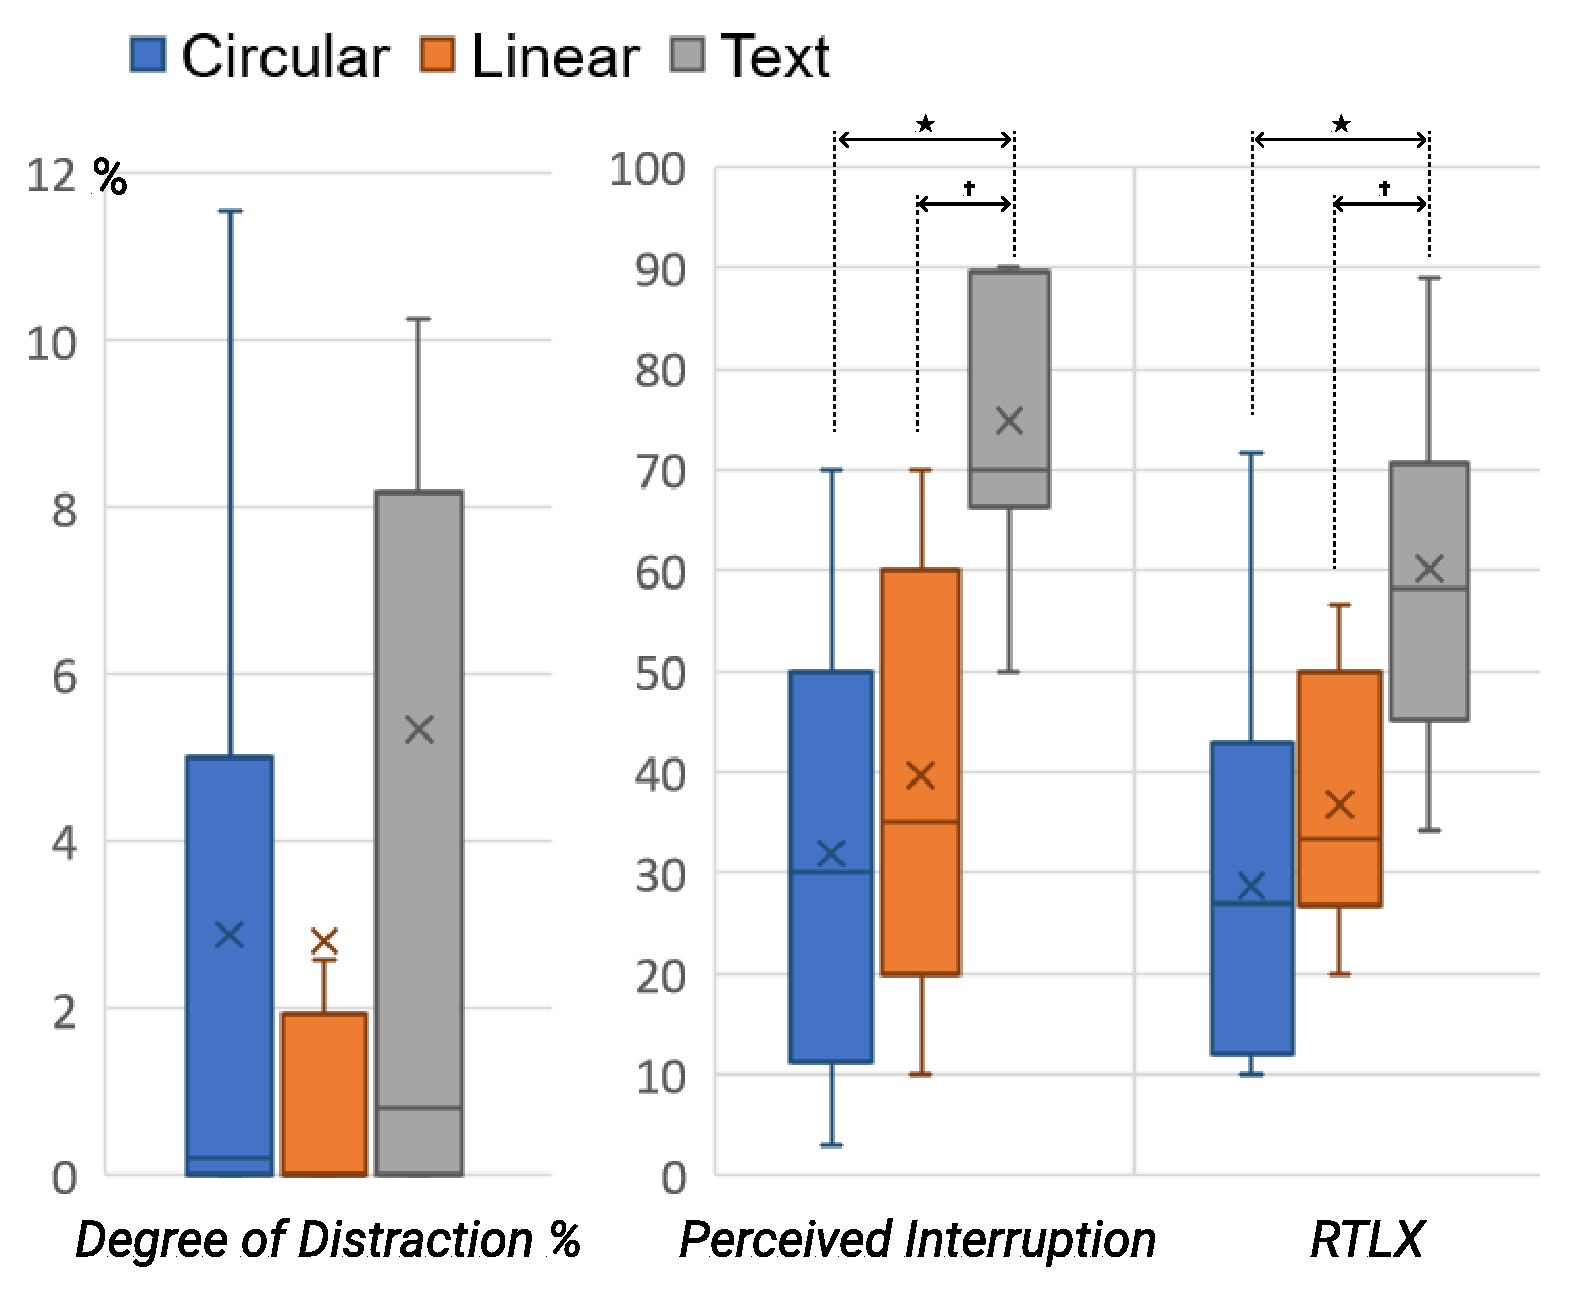
\includegraphics[width=\linewidth]{\Pic{study1/study1_box_quality_conversation.pdf}}
  \caption{Quality of conversation}
  \label{fig:Progressbar:study1:box_results_distraction}
\end{subfigure}%
\begin{subfigure}{0.57\textwidth}
  \centering
  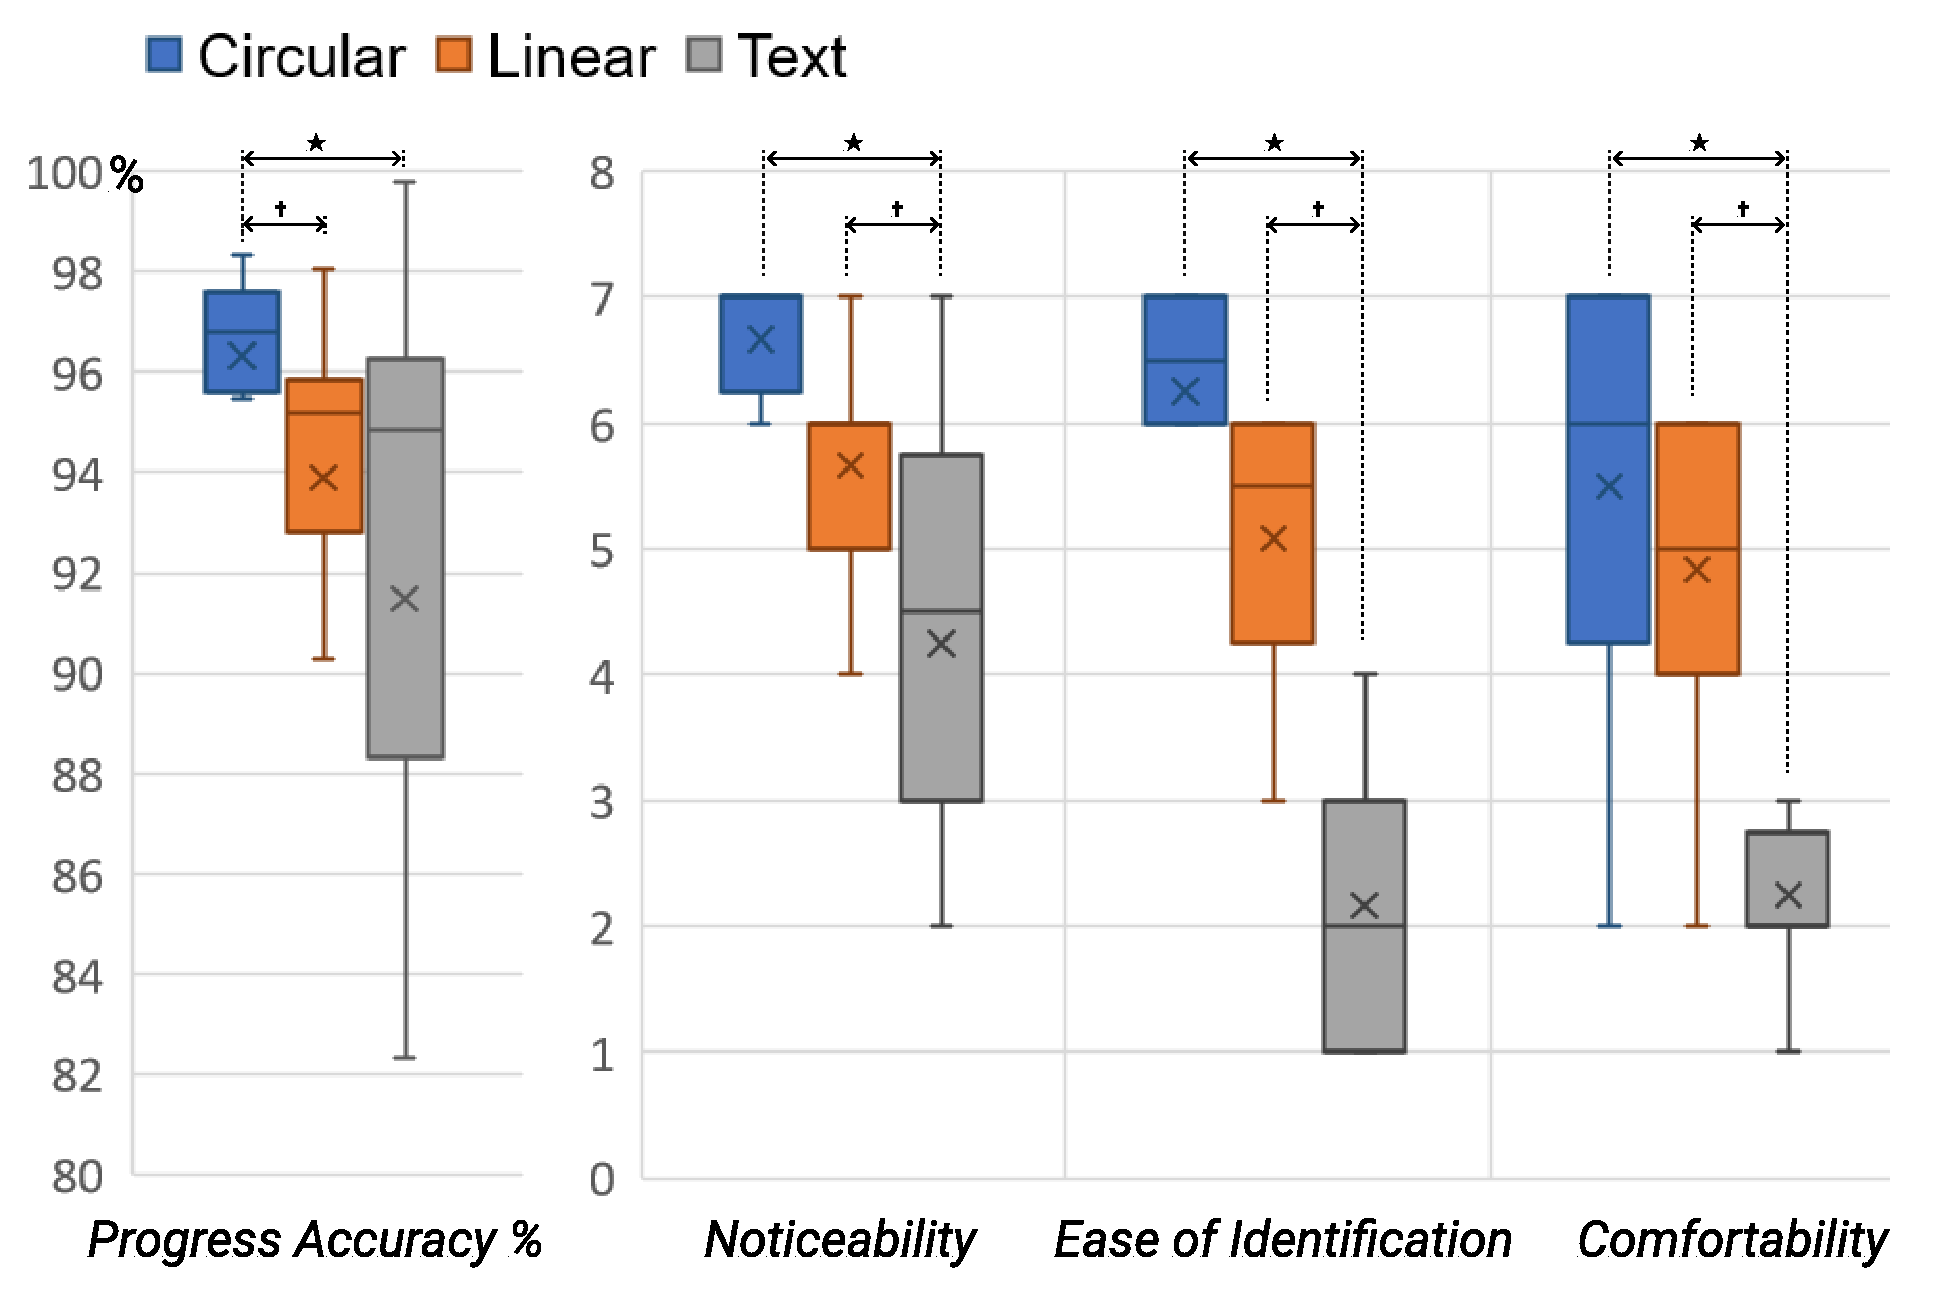
\includegraphics[width=\linewidth]{\Pic{study1/study1_box_progress_perception.pdf}}
  \caption{Progress perception}
  \label{fig:Progressbar:study1:box_results_recognition}
\end{subfigure}

\caption[Average performance in \studyone{}]{Measures in the simulated conversation setting (N = 12). \significantI{} and \significantII{} represent significant (\pval{<0.05}) post-hoc tests and  $\times$ inside box plot represents the mean value point. See \autoref{tab:Progressbar:study1:mean_results_recognition} and \autoref{tab:Progressbar:study1:mean_results_distraction} for details. }
\label{fig:Progressbar:study1:box_results}
\end{figure*}




\subsubsection*{Quality of conversation (primary task performance).}

\autoref{fig:Progressbar:study1:box_results_distraction} (\autoref{tab:Progressbar:study1:mean_results_distraction}) provides a summary of the measures.

\begin{table*}[hptb]
\centering
\caption[Primary task performance in \studyone{}]{Quality of conversation in simulated conversation setting (N = 12). Colored bars show the relative value of each measure for different progress \type{s}. \significantI{} and \significantII{} represent significant (\pval{<0.05}) post-hoc tests.}
\label{tab:Progressbar:study1:mean_results_distraction}
\small
\begin{tabular}{@{}l|ll|ll|ll@{}}
\toprule
\multicolumn{1}{r}{Measure} &
  \multicolumn{2}{c}{\distractionDigreee{} \%} &
  \multicolumn{2}{c}{\perceivedInterruption{}} & 
  \multicolumn{2}{c}{\perceivedTaskLoad{}} \\ \cmidrule(l){2-7} 
\multicolumn{1}{l}{Format} &
  \multicolumn{1}{l}{M} &
  \multicolumn{1}{l}{SD} &
  \multicolumn{1}{l}{M} &
  \multicolumn{1}{l}{SD} &
  \multicolumn{1}{l}{M} &
  \multicolumn{1}{l}{SD} \\ \midrule
  
\Circularbar{} & 
\databar{7}{2.88} & 4.74 &
\databar{80}{31.92}\significantI{} & 23.42 & 
\databar{70}{28.75}\significantI{} & 18.82 \\

\Linearbar{} & 
\databar{7}{2.81} & 7.47 & 
\databar{80}{39.75}\significantII{} & 22.32 & 
\databar{70}{36.81}\significantII{} & 12.58  \\

\Textbar{} & 
\databar{7}{5.35} & 10.75 & 
\databar{80}{74.92}\significantI{}\significantII{} & 13.55 &   
\databar{70}{60.21}\significantI{}\significantII{} & 16.54  \\
\bottomrule
\end{tabular}
\end{table*}

\factor{Objective measure - \distractionDigreee{}} 

Despite there being no significant difference (\friedman{2}{3.257}{=0.196}{0.703}) among progress \type{s}, \textbar{} registered the highest average value for \distractionDigreee{}.

\factor{Subjective measures - \perceivedInterruption{} and \perceivedTaskLoad{}}

Overall, \circularbar{} recorded lower \perceivedInterruption{} and \perceivedTaskLoad{}. Repeated-measures ANOVAs revealed significant effects of \perceivedInterruption{} (\anovawef{2}{22}{21.026}{<0.001}{0.657}) and \perceivedTaskLoad{} (\anovawef{2}{22}{16.646}{<0.001}{0.602}). Post-hoc analyses disclosed that \textbar{} was significantly different (higher, \pbonf{<0.01}) from \linearbar{} and \circularbar{} in terms of \perceivedInterruption{} and \perceivedTaskLoad{}. Results for individual indices of \perceivedTaskLoad{} are presented in \autoref{fig:Progressbar:study1:nasa_tlx}. A post-hoc analysis with Bonferroni correction showed that for all measures, \circularbar{} and \linearbar{} yielded significantly lower (\pval{<0.05}) task load results than \textbar{}. However, there were no significant differences between \circularbar{} and \linearbar{}, even though \circularbar{} recorded the lowest average task loads for all measures. On all indices, including the overall score, the sorted order of task load from lower to higher was: \circularbar{} < \linearbar{} < \textbar{}.

\begin{figure}[hptb]
  \centering
  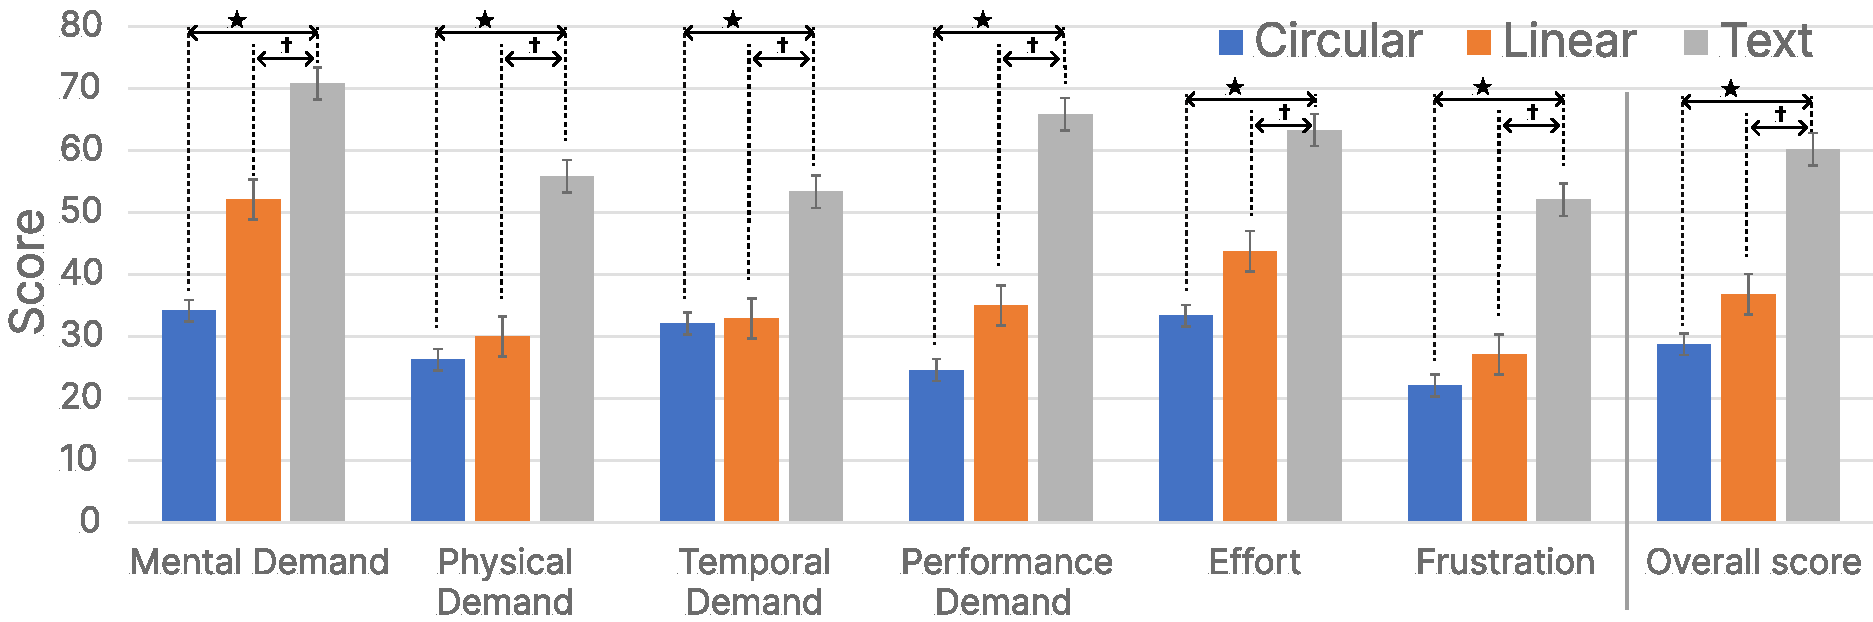
\includegraphics[width=0.9\linewidth]{\Pic{study1/study1_nasa_tlx.pdf}}
  \caption[NASA-TLX scores in \studyone{}]{NASA-TLX scores for \circularbar{}, \linearbar{}, and \textbar{}. Overall \circularbar{} had the lowest \perceivedInterruption{}. \significantI{} and \significantII{} represent significant (\pbonf{<0.05}) post-hoc tests. Error bars represent standard errors.}
  \label{fig:Progressbar:study1:nasa_tlx}	  
\end{figure}

Furthermore, all participants ranked \textbar{} as the most distracting \type{}, citing difficulty in reading or \quote{figuring out} numbers in the periphery and that it often led them to shift their focus away from the face. The majority of participants (10/12) selected \circularbar{} as the least distracting since it allowed them to perceive progress notifications without disruptions in focus.



\subsubsection*{Progress perception (notification task performance).}


\autoref{fig:Progressbar:study1:box_results_recognition} (\autoref{tab:Progressbar:study1:mean_results_recognition}) provides a summary of the measures.


\begin{table*}[hptb]
\centering
\caption[Secondary task performance in \studyone{}]{Progress perception measures in the simulated conversation setting (N = 12). Colored bars show the relative value of each measure for different progress \type{s}. \significantI{} and \significantII{} represent significant (\pbonf{<0.05}) post-hoc tests.}
\label{tab:Progressbar:study1:mean_results_recognition}
\small
\begin{tabular}{@{}l|ll|ll|ll|ll@{}}
\toprule
\multicolumn{1}{r}{Measure} &
  \multicolumn{2}{c}{\progressAccuracy{} \%} &
  \multicolumn{2}{c}{\noticeability{}} &
  \multicolumn{2}{c}{\perceivedEaseIdentification{}} &
  \multicolumn{2}{c}{\comfortability{}} \\ \cmidrule(l){2-9} 
\multicolumn{1}{l}{Format} &
  \multicolumn{1}{l}{M} &
  \multicolumn{1}{l}{SD} &
  \multicolumn{1}{l}{M} &
  \multicolumn{1}{l}{SD} &
  \multicolumn{1}{l}{M} &
  \multicolumn{1}{l}{SD} &
  \multicolumn{1}{l}{M} &
  \multicolumn{1}{l}{SD} \\ \midrule
  
\Circularbar{} & 
\databarrel{100}{80}{96.32}\significantI{}\significantII{} & 2.15 & 
\databar{7}{6.67}\significantI{}\significantII{} & 0.65 &
\databar{7}{6.25}\significantI{} & 1.14 & 
\databar{7}{5.50}\significantI{} & 1.68 \\

\Linearbar{} & 
\databarrel{100}{80}{93.89}\significantI{} & 3.82 & 
\databar{7}{5.67}\significantII{} & 0.99 & 
\databar{7}{5.08}\significantII{} & 1.17 & 
\databar{7}{4.83}\significantII{} & 1.19 \\

\Textbar{} & 
\databarrel{100}{80}{91.47}\significantII{} & 8.71 & 
\databar{7}{4.25}\significantI{} & 1.66 & 
\databar{7}{2.17}\significantI{}\significantII{} & 1.12 & 
\databar{7}{2.25}\significantI{}\significantII{} & 0.75 \\
\bottomrule
\end{tabular}
\end{table*}


\factor{Objective measure - \progressAccuracy{}} 

Overall, when participants maintained eye contact, the accuracy of progress identification dropped significantly for \textbar{} (\range{68.2}{99.8}) compared to \circularbar{} (\range{90.2}{98.3}) or \linearbar{} (\range{83.5}{98.1}). The Friedman test disclosed a significant effect (\friedman{2}{10.167}{=0.006}{0.618}) of \type{}. Surprisingly, post-hoc analysis indicated that \circularbar{} was significantly higher (\pbonf{<0.05}) than \linearbar{} and \textbar{} in terms of \progressAccuracy{}.
 
Notably, \textbar{} registered the highest variation in average accuracy, as participants' estimation errors were either very high or very low. All participants found it \quote{very difficult} to recognize and distinguish digits, as they appeared \quote{blurry} or \quote{hazy} when not looking at them directly. Specifically, they found \quote{curved} numbers (e.g., 3, 6, 8, 9) harder to recognize than \quote{pointy} ones (e.g., 1, 4). Nonetheless, two participants could achieve almost full accuracy for \textbar{} while focusing on the face, indicating individual differences in the ability to read text in the paracentral vision. Similarly, a few participants found the extreme ends of \linearbar{} (further away from the central vision) harder to read. Conversely, most participants perceived that the \circularbar{} was easier to correctly recognize the position of, as it was larger and had an additional element of \quote{angle}, e.g., 25\% is at a 90\textdegree{} angle from the center, which made the progress position more obvious.


\factor{Subjective measures - \noticeability{}, \perceivedEaseIdentification{}, and \comfortability{}}

\Circularbar{} recorded the highest average ratings for \noticeability{}, \perceivedEaseIdentification{}, and \comfortability{}. Friedman tests revealed significant effects of \noticeability{} (\friedman{2}{14.6}{<0.001}{0.388}),  \perceivedEaseIdentification{} (\friedman{2}{21.56}{<0.001}{0.307}), and \comfortability{} (\friedman{2}{16.13}{<0.001}{0.578}). Post-hoc analyses showed that \circularbar{} was significantly different (higher, \pbonf{<0.05}) from both \linearbar{} and \textbar{} in terms of \noticeability{}. Similarly, \textbar{} was significantly different (lower, \pbonf{<0.05}) than \linearbar{} and \circularbar{} in terms of \perceivedEaseIdentification{} and \comfortability{}.

The majority (10/12) of participants indicated that the \circularbar{}, which appears around the face with a larger area, was more noticeable than the \textbar{} or \linearbar{}, making it easier for them to identify the progress.



\subsubsection*{Preference}

The majority of participants (10/12) ranked \circularbar{} as their most preferred progress type, with \textbar{} being the least preferred. In our interview, participants reported that the surrounding shape of the \circularbar{} allowed them to identify the displayed progress without moving their gaze\footnote{This was further confirmed by visualizing the gaze trajectory as well.}, making it more comfortable to look at while maintaining eye contact. Additionally, the \circularbar{} resembled the familiar \quote{clock} with the progress shown at an \quote{angle}. Given its larger size, they were able to perceive the progress notifications with greater accuracy.

The remaining participants (2/12) who chose the \linearbar{} as their preferred option reported that the fixed location of the \linearbar{} allowed them to track progress values more easily than the \circularbar{} since progress values could appear anywhere around the face.

All participants chose the \textbar{} as the least preferred option, stating that the \textbar{} was \quote{difficult to decipher} (i.e., distinguish digits) and required them to exert more effort to interpret the numbers (in paracentral and near-peripheral vision) while keeping their gaze on the face.

\subsection{Discussion}

Surprisingly, evidence suggests that \textbar{} does not provide higher accuracy, as \circularbar{} demonstrated significantly higher \progressAccuracy{} and \perceivedEaseIdentification{} than \textbar{}. Text can only be clearly perceived when presented within central vision \cite{rayner_eye_1998, ishiguro_peripheral_2011}, which was not the case for our \textbar{} condition.

Given that both \circularbar{} and \linearbar{} have simpler visual patterns than text \cite[Ch~6]{wickens_engineering_2015}, and that shapes and colors are recognized at a greater angle than text \cite[Ch~C.9]{ishiguro_peripheral_2011, panero1979human}, the \circularbar{} and \linearbar{} were easier to recognize in paracentral and near-peripheral vision than the \textbar{}.

As expected, the \circularbar{} had significantly lower \perceivedInterruption{}, \perceivedTaskLoad{}, and a lower \distractionDigreee{} than \textbar{}. We lack evidence to draw the same conclusion for the comparison between \circularbar{} and \linearbar{}.

Comparing \textbar{} with \circularbar{}, there appears to be a trade-off between accuracy and maintaining (uninterrupted) eye contact for \textbar{}. A majority (83\%) of participants preferred the \circularbar{}, in line with the results showing that \circularbar{} resulted in the lowest distraction levels and highest accuracy while participants maintained uninterrupted eye contact. Hence, the \circularbar{} is the ideal choice for presenting progress/task completion reminders when users need to maintain their focus on a primary visual target.























\section{Study 2: Identify how the presentation type of progress notifications affect face-to-face conversations}
\label{sec:Progressbar:study2}

In this study, we complemented \studyone{} with a more realistic setting in which a pair of participants (\receiver{} and \observer{}, \autoref{sec:Progressbar:study2:apparatus}) engaged in a conversation. We initially explored the optimal form of \persistence{} (i.e., whether progress is presented \continuous{ly} or \intermittent{ly} on the OHMD) for progress bar design through a pilot study with 4 participants, then subsequently conducted a formal study with 12 participants.


\subsection{Apparatus}
\label{sec:Progressbar:study2:apparatus}

As shown in \autoref{fig:Progressbar:study2:apparatus}, the same HoloLens2 was used by the \receiver{}, where the progress information was displayed in an observer-locked alignment with the face of the \observer{}. This observer-locked alignment was implemented using Windows' FaceTracker\footnote{\url{https://docs.microsoft.com/en-us/uwp/api/Windows.Media.FaceAnalysis.FaceTracker}} API and Unity's viewport to world mapping\footnote{\url{https://docs.unity3d.com/ScriptReference/Camera.ViewportToWorldPoint.html}} at a fixed distance with a tracking rate of 10Hz. To minimize misalignments of progress bars with respect to the \observer{} due to tracking errors, we asked trained \observer{s} to limit their \textit{sudden} head movements during conversations. The gaze cursor was removed for realistic effects, as they are rarely used in real conversations. The distance between the \receiver{} and \observer{} was maintained at 1.5 m, replicating \studyone{}. 


\begin{figure}[hptb]
  \centering
  \includegraphics[width=0.8\linewidth]{\Pic{study2/study2_apparatus.pdf}}
  \caption[The apparatus in \studytwo{}]{The \receiver{} is wearing the OHMD while engaging in a conversation with the \observer{}. The \receiver{} sees three progress \type{s} in three conditions. From left to right, the top figure depicts the progress bars: \circularbar{}, \linearbar{}, and \textbar{}.}
  \label{fig:Progressbar:study2:apparatus}
\end{figure}


\subsection{Tasks}
 
A \receiver{} and \observer{} pair engaged in a face-to-face conversation on a given topic (\autoref{fig:Progressbar:study2:apparatus}) provided by the researcher. The topics were selected from the CAE speaking test \cite{cambridge2008speaking} (e.g., ``What are the advantages and disadvantages of shopping by computer?''), similar to those used by Mayer et al. \cite{mayer_evaluating_2018} and Rzayev et al. \cite{rzayev_effects_2020}. We limited each conversation session to 6 minutes, ensuring that participants had sufficient time to engage in the conversation and attend to progress notifications. 

In addition to engaging in the conversation as the primary task, both the \receiver{} and the \observer{} had secondary tasks. We asked the \receiver{} to end the conversation smoothly when the progress bar reached 100\% and then stand up. The \observer{} was instructed to observe whether the \receiver{} paid attention to the conversation and to rate the eye contact and naturalness of the conversation after the discussion. Neither was aware of the other's secondary task.

\subsection{Progress bar design}

\subsubsection*{General design}

In order to establish the conversation flow, we started the progress bar from 0\% 30 seconds after the conversation began. The progress bars then incremented at a uniform speed of 1\% every 3 seconds, reaching 100\% in 5 minutes. After this, the progress bar remained on view for an additional 45 seconds before it informed the \receiver{} to stop the session.

\subsubsection*{Pilot study to determine the persistence}
\label{study2:pilot_persistance}

We tested two kinds of \persistence{} for progress notification presentation: \continuous{} and \intermittent{}. The \continuous{} progress bar remained on the screen, whereas the \intermittent{} progress bar appeared only when the progress value reached multiples of 10\% (i.e., 10\%, 20\% ...), staying on the screen for 3 seconds each time it appeared. The appearance interval and staying duration were determined by several pilots.

The pilot results with 4 participants showed that the \continuous{} \persistence{} on screen was perceived as more distracting and was less preferred compared to the \intermittent{} one. Participants reported that they tended to \quote{constantly check the progress}, as the value was continuously changing, and they did not intend to do this, especially when they had more time left for conversation. This constant checking disrupted their \quote{train of thoughts}. As for preference, most participants (3/4) preferred \intermittent{}, as it highlighted progress with minimal distraction. This finding aligns with the literature \cite{tanveer_rhema_2015, ofek_reducing_2013} that recommends sparse feedback to reduce distraction from the primary task during multitasking. The only participant who reported more distraction from the \continuous{} still preferred it due to the accurate time tracking. Based on the pilot results, we decided to use only the \intermittent{} \persistence{} in the formal study.

\subsection{Participants}
\label{sec:Progressbar:study2:participants}
 
The \receiver{s} were 12 participants (7 females, mean age = 22.4, SD = 2.5) recruited from the university community, following the same standards as \studyone{} (\autoref{sec:Progressbar:study1:participants}). The \observer{s} were two volunteers (2 males, mean age = 24.5) from the same community and were trained to manage the conversation to ensure fluid continuity. They were fluent in English and acted as conversation partners. The \observer{s} were not aware of the study conditions. None of them participated in \studyone{}. 


\subsection{Procedure}
 
The study was conducted in a quiet room under indoor lighting conditions to provide a consistent user experience. When the \receiver{s} arrived, they were briefed about the study process and signed the consent form. They then familiarized themselves with the OHMD and the three types of progress bars. They were also informed about the intermittent appearance, expected duration, and frequency of the progress bar during the conversation. They were reminded to focus on the conversation while attending to the progress bars. 

When the \receiver{} was comfortable with the setup, the \observer{} was guided to the same room and seated on the opposite side of a table (see \autoref{fig:Progressbar:study2:apparatus}) such that they were 1.5 m apart from each other. They were given a practice topic to engage in a conversation without any progress bar displayed on the OHMD for 3-4 minutes. They then engaged in three conversation sessions with three types of progress bars. After each conversation, the \receiver{} removed the OHMD, and the participant pair filled out the questionnaires (\autoref{sec:Progressbar:study2:measures}) separately. After completing the questionnaire, a 2-minute break was provided before proceeding to the next condition. In the end, both participants filled out a questionnaire on their overall experience and separately attended the semi-structured interview sessions. These sessions captured the \receiver{'s} perception of progress indication, their experience of receiving progress notifications, and the \observer{'s} perception of the conversation. The study took approximately 80 minutes per participant pair.

\subsection{Study design}

We tested three conditions: the \circularbar{}, \linearbar{}, and \textbar{} using a within-subject design, which was fully counterbalanced.



\subsubsection*{Measures}
\label{sec:Progressbar:study2:measures}

In this study, we collected subjective measures of the quality of two-way conversation and the \receiver{'s} perception towards the different progress \type{s}. At the end of the study, we also collected the \receiver{s'} preference for different progress types.

\factor{Quality of the conversation}
To measure the quality of the conversation, we employed three categories of measures: attention and concentration, eye contact, and naturalness; these were gathered from both the \receiver{'s} (\prefixReceiver{}) and \observer{'s} (\prefixObserver{}) perspectives. These measures were adapted from McAtamney et al.'s study \cite{mcatamney_examination_2006}, but the 5-point Likert scales were changed to 7-point scales (1 = Strongly Disagree, 7 = Strongly Agree) to increase sensitivity and ensure consistency with other measures (see \autoref{tab:Progressbar:study2:scales_conversation} for the list of measures used in the study).


\begin{table*}[hptb]
\centering
\caption[Additional measures on conversation quality]{Aspects and measures on conversation behavior of \receiver{} from the \receiver{} \prefixReceiver{} and the \observer{} \prefixObserver{} point of views (source: \cite{mcatamney_examination_2006}).}
\label{tab:Progressbar:study2:scales_conversation}
\small
\begin{tabular}{l p{0.7\textwidth} }
\toprule
Aspect on conversation                     & Measures                  \\ \midrule
\multirow{2}{*}{\begin{tabular}[c]{@{}l@{}} Attention and \\concentration\end{tabular}} 

& \b{AC1}: {\prefixReceiver{} `When the other person was speaking, I was always listening to them'} / {\prefixObserver{} `When I was speaking, I think the other person was always listening to me'} \\
                                             & \b{AC2}: {\prefixReceiver{} `I was always concentrating on the conversation'} / {\prefixObserver{} `I think the other person was always concentrating on the conversation'} \\ \midrule
\multirow{2}{*}{Eye contact}                 & \b{EC1}: {\prefixReceiver{} `When I was speaking, my attention was towards the other person'} / {\prefixObserver{} `When the other person was speaking their attention was towards me'} \\
                                             & \b{EC2}: {\prefixObserver{} `When I was speaking the other person maintained eye contact'}           \\ \midrule
\multirow{2}{*}{Natural behavior}            & \b{NB1}: {\prefixReceiver{} `I acted naturally at all times during the conversation'} /{\prefixObserver{} `The other person acted naturally at all times during the conversation'}  \\
                                             & \b{NB2}: {\prefixReceiver{} `I felt relaxed during the conversation'}/ {\prefixObserver{} ` The other person appeared relaxed during the conversation'}  \\ \bottomrule
\end{tabular}
\end{table*}


\factor{Progress perception}  
Similar to \studyone{}, the perception of the progress bar was evaluated by the \receiver{s} after each condition, using measures of \noticeability{} and \comfortability{}. Additionally, they evaluated \perceivedEffectiveness{} in delivering the current progress with a 7-point Likert scale (1 = Very Ineffective, 7 = Very Effective). 


\subsection{Results}

During the study, each participant completed three conditions, resulting in a total of 36 (= 3 x 12) conversations. \autoref{fig:Progressbar:study2:box_progress_perception} (\autoref{tab:Progressbar:study2:measures_progress}) and \autoref{fig:Progressbar:study2:box_results} (\autoref{tab:Progressbar:study2:measures_conversation}) represent the summary of measures. One \observer{} conversed with 8 \receiver{s}, while the other \observer{} conversed with the remaining 4 \receiver{s}.



\subsubsection*{Quality of the conversation (primary task performance).\\}

We analyzed the subjective ratings of attention and concentration (AC), eye contact (EC), and natural behavior (NB), from both the \receiver{'s} (\prefixReceiver{}) and \observer{'s} (\prefixObserver{}) perspectives. There was a significant difference in \i{NB2} from the \receiver{'s} perspective (Friedman test, \friedman{2}{10.563}{=0.005}{0.781}), yet the \textbar{} (\meansd{4.67}{1.56}) was not significantly lower than the \circularbar{} (\meansd{5.50}{0.91}, \pbonf{=0.096}) and \linearbar{} (\meansd{5.67}{0.78}, \pbonf{=0.063}). Besides this measure, there were no significant differences for other measures. The detailed results are summarized in \autoref{fig:Progressbar:study2:box_results} (\autoref{tab:Progressbar:study2:measures_conversation}).

\begin{figure*}[hptb]
\centering

\begin{subfigure}{0.9\textwidth}
  \centering
  \includegraphics[width=\textwidth]{\Pic{study2/study2_box_receiver.pdf}}
  \caption{Perceived ratings by \receiver{} \prefixReceiver{}}
  \label{fig:Progressbar:study2:box_results_receiver}
\end{subfigure}
\begin{subfigure}{0.9\textwidth}
  \centering
  \includegraphics[width=\textwidth]{\Pic{study2/study2_box_observer.pdf}}
  \caption{Perceived ratings by \observer{} \prefixObserver{}}
  \label{fig:Progressbar:study2:box_results_observer}
\end{subfigure}

\caption[Primary task performance in \studytwo{}]{Perceived rating on progress \type{s} by \receiver{} \prefixReceiver{} and \observer{} \prefixObserver{} (N = 12).  $\times$ inside the box plot represents the mean value point. See  \autoref{tab:Progressbar:study2:measures_conversation} for details. }
\label{fig:Progressbar:study2:box_results}
\end{figure*}

\begin{table*}[hptb]
\centering
\caption[Average primary task performance in \studytwo{}]{Perceived rating in conversation setting (N = 12) by \receiver{} \prefixReceiver{} and \observer{} \prefixObserver{}. Here \i{C} = \Circularbar{}, \i{L} = \Linearbar{}, and \i{T} = \Textbar{}. Colored bars show the relative value of each measure for different progress \type{s}. \significantII{} and \significantIII{} represent non-significant (\pbonf{>0.05}) yet \pbonf{<0.10} post-hoc tests.}
\label{tab:Progressbar:study2:measures_conversation}

\scalebox{0.9}{
\begin{tabular}{@{}l|ll|ll|ll|ll|ll|ll@{}}
\toprule
\multicolumn{1}{r}{Measure} &
  \multicolumn{2}{c}{AC1} &
  \multicolumn{2}{c}{AC2} &
  \multicolumn{2}{c}{EC1} &
  \multicolumn{2}{c}{EC2}  &
  \multicolumn{2}{c}{NB1} & 
  \multicolumn{2}{c}{NB2} \\ \cmidrule(l){2-13} 
\multicolumn{1}{l}{Format} &
  \multicolumn{1}{l}{M} &
  \multicolumn{1}{l}{SD} &
  \multicolumn{1}{l}{M} &
  \multicolumn{1}{l}{SD} &
  \multicolumn{1}{l}{M} &
  \multicolumn{1}{l}{SD} &
  \multicolumn{1}{l}{M} &
  \multicolumn{1}{l}{SD} &
  \multicolumn{1}{l}{M} &
  \multicolumn{1}{l}{SD} &
  \multicolumn{1}{l}{M} &
  \multicolumn{1}{l}{SD} \\ \midrule
  
\prefixReceiver{} \i{C} & 
\databar{7}{6.00} & 1.28 & 
\databar{7}{5.50} & 1.31 &
\databar{7}{5.83} & 0.94 & 
- & - & 
\databar{7}{5.17} & 1.27 & 
\databar{7}{5.50}\significantII{} & 0.91 \\

\prefixReceiver{} \i{L} & 
\databar{7}{6.08} & 1.00 & 
\databar{7}{5.83} & 1.19 & 
\databar{7}{5.92} & 1.17 & 
- & - & 
\databar{7}{5.58} & 1.24 & 
\databar{7}{5.67}\significantIII{} & 0.78  \\

\prefixReceiver{} \i{T} & 
\databar{7}{6.17} & 1.03 & 
\databar{7}{5.75} & 0.87 & 
\databar{7}{5.92} & 1.17 & 
- & - & 
\databar{7}{5.25} & 1.22 &   
\databar{7}{4.67}\significantII{}\significantIII{} & 1.56  \\
\midrule

\prefixObserver{} \i{C} & 
\databar{7}{6.67} & 0.49 & 
\databar{7}{6.50} & 0.65 &
\databar{7}{6.33} & 0.78 & 
\databar{7}{6.25} & 0.75 & 
\databar{7}{6.08} & 0.67 & 
\databar{7}{6.50} & 0.67 \\

\prefixObserver{} \i{L} & 
\databar{7}{6.50} & 0.67 & 
\databar{7}{6.67} & 0.49 & 
\databar{7}{6.67} & 0.49 & 
\databar{7}{6.25} & 0.62 & 
\databar{7}{6.25} & 0.62 & 
\databar{7}{6.42} & 0.90  \\

\prefixObserver{} \i{T} & 
\databar{7}{6.50} & 0.91 & 
\databar{7}{6.67} & 0.49 & 
\databar{7}{6.42} & 0.67 & 
\databar{7}{6.17} & 0.39 &  
\databar{7}{6.33} & 0.65 &   
\databar{7}{6.67} & 0.65  \\

\bottomrule
\end{tabular}
}
\end{table*}


At the start, the \observer{s} felt \quote{uncomfortable} and \quote{awkward} talking with \receiver{s} who were wearing \quote{bulky} OHMDs but eventually found it more natural once the conversation began. They mentioned that using \quote{spectacle-like} OHMDs in a casual conversation would be socially acceptable, as it would be similar to the use of smartphones when engaged in a conversation, but still considered \quote{rude} in a professional setting. This could be because the Microsoft Hololens2 is still too bulky and does not resemble regular glasses. We expect this problem to be mitigated with more lightweight and natural-looking glasses such as the North Focals\footnote{\url{https://www.theverge.com/2019/2/14/18223593/focals-smart-glasses-north-review-specs-features-price}} smart glasses.

From the \observer{'s} point of view, they did not notice any significant differences in the naturalness of conversation among sessions. Sometimes, they noticed that the \receiver{s'} gaze \quote{moved to the corner}, but they assumed the \receiver{s} were thinking, and this was perceived as natural.


\subsubsection*{Progress perception (notification task performance).\\}

The post-hoc analysis showed that the \circularbar{} had the highest \noticeability{} and \perceivedEffectiveness{} compared with the \linearbar{} and \textbar{}, and a higher \comfortability{} compared with the \textbar{}. The Friedman test revealed significant differences between progress \type{s} in terms of \noticeability{} (\friedman{2}{8.600}{=0.014}{0.580}), \comfortability{} (\friedman{2}{6.324}{=0.042}{0.515}), and \perceivedEffectiveness{} (\friedman{2}{8.424}{=0.015}{0.696}). The differences between \circularbar{} and \linearbar{} in terms of \noticeability{} and \perceivedEffectiveness{} were significant (\pbonf{<0.05}), whereas the difference in terms of \comfortability{} was not significant (\pbonf{=0.098}). The detailed results are summarized in \autoref{fig:Progressbar:study2:box_progress_perception} (\autoref{tab:Progressbar:study2:measures_progress}).


\begin{figure}[hptb]
\centering
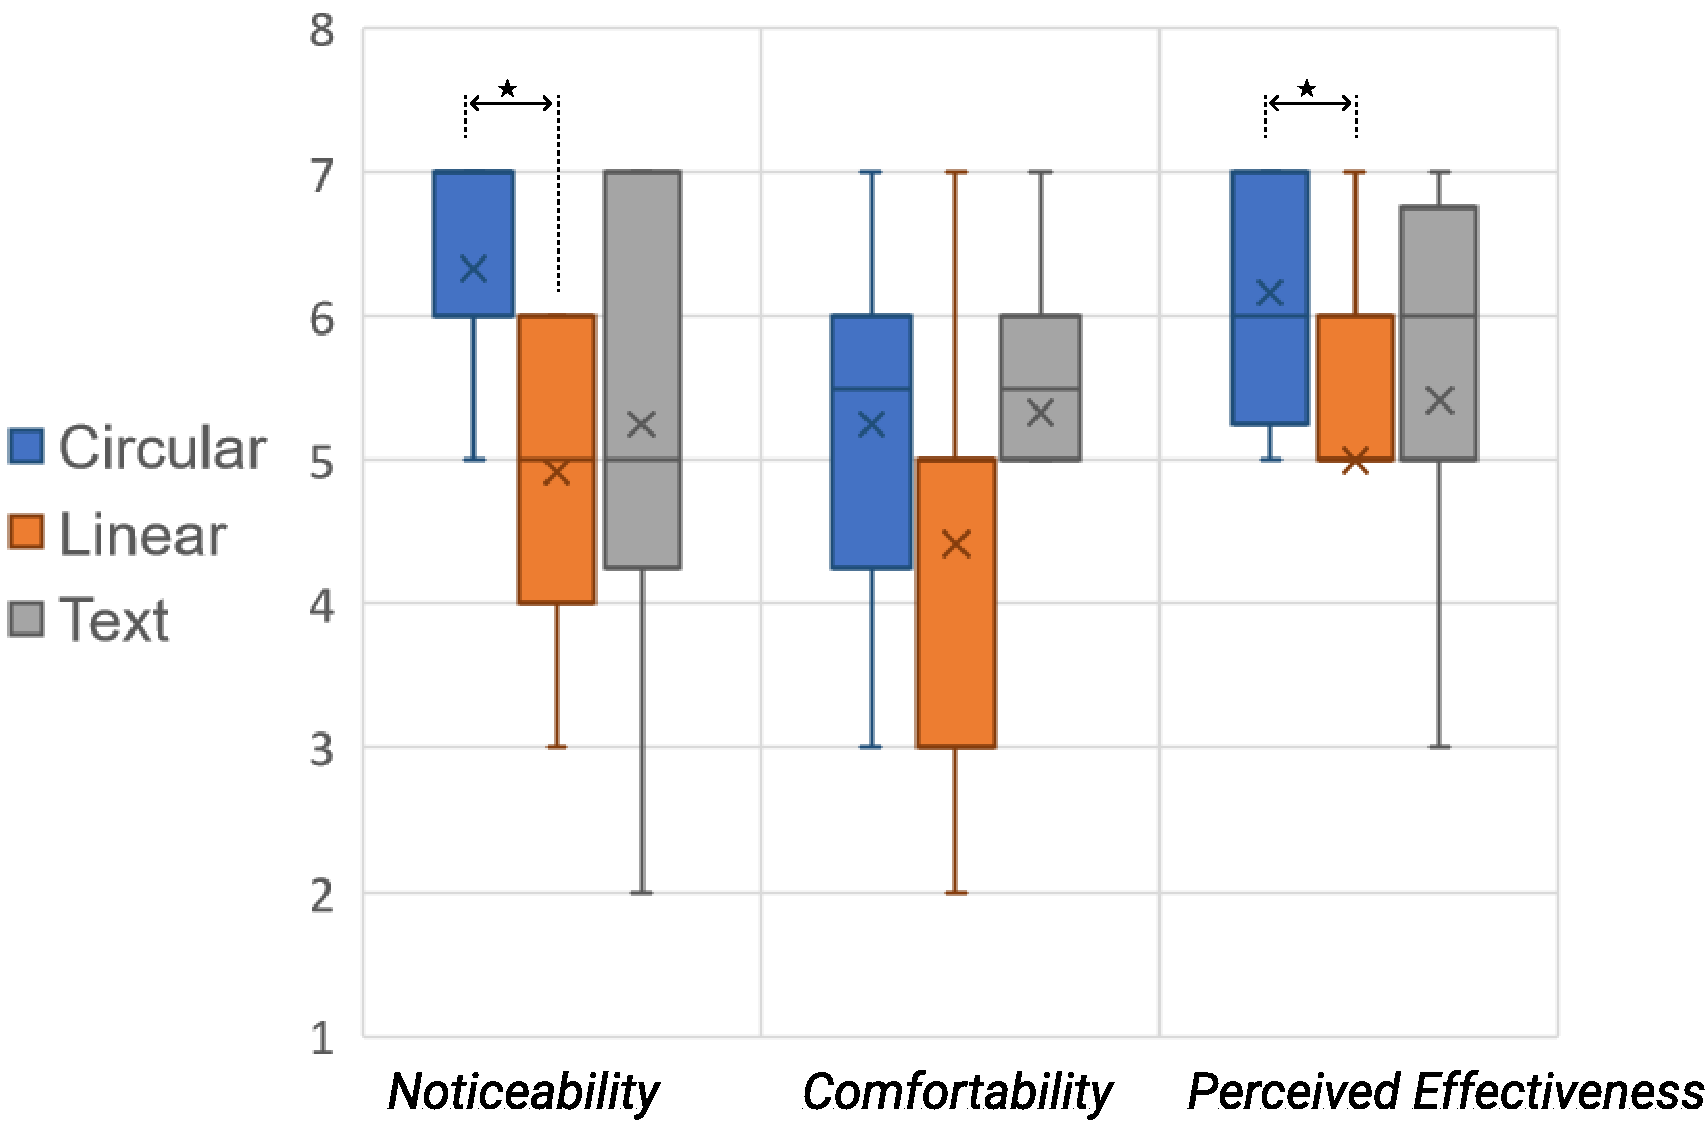
\includegraphics[width=0.65\linewidth]{\Pic{study2/study2_box_progress_perception.pdf}}
\caption[Secondary task performance in \studytwo{} by \receiver{}]{Perceived rating on progress \type{s} by \receiver{} (N = 12). \significantI{} represents significant (\pbonf{<0.05}) post-hoc tests and $\times$ inside box plot represents the mean value point. See \autoref{tab:Progressbar:study2:measures_progress} for details. }
\label{fig:Progressbar:study2:box_progress_perception}
\end{figure}


\begin{table*}[hptb]
\centering
\caption[Average secondary task performance in \studytwo{}]{Perceived rating on progress \type{s} (N = 12). Colored bars show the relative value of each measure for different progress \type{s}. \significantI{} represents significant (\pval{<0.05}) post-hoc tests. \significantII{} and \significantIII{} represents non-significant (\pbonf{>0.05}) yet \pbonf{<0.10} post-hoc tests.}
\label{tab:Progressbar:study2:measures_progress}
\small
\begin{tabular}{@{}l|ll|ll|ll@{}}
\toprule
\multicolumn{1}{r}{Measure} &
  \multicolumn{2}{c}{\noticeability{}} &
  \multicolumn{2}{c}{\comfortability{}}  &
  \multicolumn{2}{c}{\perceivedEffectiveness{}} \\ \cmidrule(l){2-7} 
\multicolumn{1}{l}{Format} &
  \multicolumn{1}{l}{M} &
  \multicolumn{1}{l}{SD} &
  \multicolumn{1}{l}{M} &
  \multicolumn{1}{l}{SD} &
  \multicolumn{1}{l}{M} &
  \multicolumn{1}{l}{SD} \\ \midrule
  
\Circularbar{} & 
\databar{7}{6.33}\significantI{} & 0.99 &
\databar{7}{5.25}\significantII{} & 1.14 & 
\databar{7}{6.17}\significantI{} & 0.84  \\

\Linearbar{} & 
\databar{7}{4.92}\significantI{} & 1.17 & 
\databar{7}{4.42}\significantII{}\significantIII{}  & 1.44 & 
\databar{7}{5.00}\significantI{} & 1.54 \\

\Textbar{} & 
\databar{7}{5.25} & 1.66 & 
\databar{7}{5.33}\significantIII{} & 1.30 & 
\databar{7}{5.42} & 1.56 \\

\bottomrule
\end{tabular}
\end{table*}


During the interview, all \receiver{s} mentioned that although they needed \quote{a short time} to glance at the progress bars, they did not have to look away from their partner for the \circularbar{} condition. However, for the \textbar{} and \linearbar{}, they needed to look at the top of the screen to check the progress.
While they could still maintain eye contact with the \observer{}, a few \receiver{s} (4/12) acknowledged that the sudden appearance of progress bars distracted them from their conversations. This distraction was relatively subtle, as the progress bars did not block their view of the \observer{} and only appeared intermittently. But they felt time pressure when the progress reached the end.


\subsubsection*{\Receiver{s'} preference}
\label{sec:Progressbar:study2:receiver_preference}

As shown in \autoref{fig:Progressbar:study2:overall_ranking}, more than half of the participants (7/12) ranked \circularbar{} as their highest preference, while 3 participants ranked \textbar{} and 2 participants ranked \linearbar{} as their most preferred.

\begin{figure}[hptb]
  \centering
  \includegraphics[width=0.65\linewidth]{\Pic{study2/study2_preference_distraction.pdf}}
  \caption[Overall preference in \studytwo{}]{Overall preference from \receiver{'s} perspective and eye contact ranking from \observer{'s} perspective}
  \label{fig:Progressbar:study2:overall_ranking}	  
\end{figure}




During the interview, participants who preferred \circularbar{} reported that it was easier to notice. The surrounding shape and the clock-like design enabled them to easily recognize the progress while maintaining attention on their partners. Compared with the \circularbar{}, the \linearbar{} required them to shift their attention away from the partner to see the progress. The \textbar{} was even harder to notice, required more attention to read the text, and was perceived as more \quote{stressful} as it provided exact numbers.

However, some participants did not prefer \circularbar{}, mentioning that the progress position of the \circularbar{} moved around the face, so they needed more time to check where to look. The \textbar{} and \linearbar{} were in a relatively fixed position, so they only needed to focus on one area to read progress.\\ 

\textit{\Observer{s'} perception of \receiver{s'} eye contact:}
Observers did not detect many differences in eye contact among the different conditions, although they did sometimes notice the participant looking up or to the side, but they interpreted this as \quote{they were processing what was said} or \quote{thinking about what to say next}, and did not take this as a lack of eye contact. As the \linearbar{} was placed above the head, when the \receiver{} looked at it, this could have been mistaken for thinking, but overall, this behavior did not cause any discomfort to \observer{s}.

\subsection{Discussion}

Overall, the majority (7/12) of \receiver{s} chose \circularbar{} as their first preference, which is consistent with \studyone{}, thus \circularbar{} is preferred over \linearbar{} and \textbar{}, is validated in a more realistic setting.
In accordance with \studyone{}, this study showed the \circularbar{} had higher noticeability and comfortability, and was also perceived as most effective in delivering progress information.

However, some participants (3/12) perceived the \textbar{} to be more comfortable for checking progress, as they could \quote{quickly glance} at the progress without significantly affecting social engagement. These three participants chose the \textbar{} as their first preference, indicating that it could also be suitable for certain users.

Except for the relaxation measure (i.e., \textit{NB2}), there were no significant differences between progress \type{s} on conversation quality. The \circularbar{} and \linearbar{} were \textit{more relaxing} to see than \textbar{} while conversing. Thus, statistically significant evidence is lacking to support that the \circularbar{} enables greater attention toward conversations. However, qualitative feedback supports the insight that \circularbar{} minimizes attention switching between conversation partner and on-screen progress information. Multiple participants mentioned how the information shown on the \circularbar{} is \quote{immediately understandable}, due to the shape and the graphical representation, meaning that they did not have to spend too much time processing the information and could continue conversing with their partner. They also mentioned how it was very \quote{obvious}, and could thus focus more on the primary task than interpreting or anticipating the progress bar.

Overall, based on the study results, we recommend using \circularbar{} to present progress/task completion notifications in face-to-face (1:1) conversations. But there are many other social interactions such as interviews, group meetings, and public speaking where progress notifications can be used, and we need further explorations to identify the most suitable \type{} in those scenarios and how they will be moderated by the urgency and importance of such notifications.























\section{General discussion}
\label{sec:Progressbar:general_discussion}

\subsection{Study summary}

In \studyone{}, we found that when participants maintained uninterrupted eye contact in a simulated conversational setting, the \circularbar{} enabled participants to receive progress notifications with less distraction, higher noticeability, comfortability, and accuracy. The \circularbar{}, aligned with the ring-shaped paracentral and near-peripheral vision, allowed users to interpret progress values with significantly higher accuracy than the \textbar{}. This was the preferred presentation type for the majority (83\%) of participants.
In \studytwo{}, we sought to verify the results of \studyone{} in a realistic conversation setting. We found that the \circularbar{} was perceived as more effective in notifying participants of progress. Participants felt more relaxed with the \circularbar{} than with the \textbar{}, and the majority of users (58\%) preferred it.
While the general consensus favored the \circularbar{}, there are merits to the other two designs.

As previously discussed, text is the most concise and direct presentation form but requires a certain amount of visual capability for viewing. The \linearbar{} strikes a balance between noticeability and disruption but provides an uneven viewing experience: the areas of the bar closer to the region of central vision are more visible than areas of the bar that are further away. The \circularbar{} and its circular shape make it easier to focus on the central location of the primary visual target, though its larger area can also be overwhelming. We analyzed these design trade-offs for deeper insights.

\begin{figure}[hptb]

\begin{subfigure}{1\linewidth}
  \centering
  \includegraphics[width=0.72\linewidth]{\Pic{discussion/visual_perception_angles.png}}
  \caption{Visual perception angles of eyes. Source: \cite{ishiguro_peripheral_2011} (Figure~4).}
\end{subfigure}
\begin{subfigure}{1\linewidth}
  \centering
  \includegraphics[width=0.9\linewidth]{\Pic{discussion/vision_capabilities.png}}
  \caption{Capabilities of paracentral and near-peripheral vision. References: \cite{wiki_fov_2021, ishiguro_peripheral_2011, panero1979human} }	  
\end{subfigure}

\caption[Visual perception angles of eyes]{Visual perception angles and capabilities of eyes for text, shapes, and color recognition.}
\label{fig:IconNotif:discussion:visual_perception}
\end{figure}

\subsection{The role of text in secondary information display}

As depicted in \autoref{fig:IconNotif:discussion:visual_perception}, even though the paracentral and near-peripheral regions possess some capability to recognize text or symbols, it remains challenging for most participants to reliably read text using either the paracentral or near-peripheral regions alone. Therefore, displaying text entirely outside the central vision is not recommended. However, our experiment also revealed that participants could largely discern the meaning of the text information in the paracentral vision, indicating a potential to offload some tasks from the central vision. One possible design is shown in \autoref{fig:Progressbar:discussion:circular_widgets}a. By placing the words across near-peripheral, paracentral, and central vision, the likelihood of comprehending the meaning significantly increases. While the text further away from the central vision is harder to read, readers can infer their meanings by considering them in conjunction with the text displayed in the central vision based on their context. We believe this strategy can be used to display familiar phrases while preserving the central vision for primary viewing tasks. Additionally, fonts designed specifically for peripheral viewing like `Eido' \cite{bernard_new_2016} or `PeriText' \cite{ku_peritext_2019}, can be employed for displaying text in the peripheral region of the eyes.

\begin{figure}[hptb]
  \centering
  \includegraphics[width=0.9\linewidth]{\Pic{discussion/discussion_circular_widgets.pdf}}
  \caption[Applications scenarios of paracentral and near-peripheral visualization]{(a) Align important text to paracentral region, (b) Proposed \linearbar{}, (c) Use of paracentral and near-peripheral vision for a glanceable radial menu or notification display, (d) Use of paracentral vision to show  estimated arrival time. Image sources:  Flaticon.com (photo3idea\_studio), Unsplash.com, and Google Material Icons}
  \label{fig:Progressbar:discussion:circular_widgets}	  
\end{figure}



\subsection{Trade-off between circular vs. linear visualization}

We discovered that the circular shape offers a unique advantage as it mirrors the shape of our vision systems. By evenly distributing information around the central vision, it is easier for the user to maintain focus. Thus, a circle is an ideal shape for designing attention-maintaining secondary visual displays. This chapter explored one type of circular secondary information: progress updates, but this concept can be extended to other types of information. For instance, \autoref{fig:Progressbar:discussion:circular_widgets}c displays a transparent radial menu around the primary visual target. We believe such designs can help users perceive the menu options while easily maintaining visual focus. Another example is a modified notification summarizer, the `Scope', proposed by Dantzich et al. \cite{van_dantzich_scope_2002}, which leaves the center blank and puts notifications around the ring, allowing for multiple glanceable categories of notifications (\autoref{fig:Progressbar:discussion:circular_widgets}c). A similar design could also be used in presenting trip status (e.g., estimated arrival time) to users as shown in \autoref{fig:Progressbar:discussion:circular_widgets}d.

The \linearbar{}, although familiar, doesn't align well with our eyes' anatomy. However, the linear progress update visualization is more predictable as it consistently appears above the head (\autoref{sec:Progressbar:study2:receiver_preference}), thus easier for users to locate. Given that we understand the importance of progress information is not evenly distributed (more discussion in the following section): the closer to the deadline, the more critical the progress update becomes, so we could adjust the position of the \linearbar{} so that the ending segment is closer to the central vision (\autoref{fig:Progressbar:discussion:circular_widgets}b), thereby making it easier to perceive the information at the most important moments.

\subsection{Timing of progress update}

During the interview of \studytwo{}, we collected participants' feedback on the \intermittent{} \persistence{} of progress bars. Most participants (\receiver{s}) reported that they only checked the progress at the beginning and near the end of the conversation. Many of them (6/12) preferred the progress bar to appear \intermittent{ly} with a lower frequency (e.g., 25\%, 50\%, 75\%) at the beginning and to appear \intermittent{ly} with a higher frequency (e.g., 80\%, 90\%, 100\%) or even \continuous{ly} near the end. These results suggest that people's needs for checking the progress on the notification bar vary. They are particularly interested in being notified towards the end of the progress to prepare for follow-up actions. Thus, we recommend designing the \circularbar{} with a hybrid \persistence{}, supporting user customization.

\subsection{Social distance and perception of progress bars}

In realistic conversations, the distance between the \receiver{} and \observer{} can be shorter or longer than the distance we tested. When they get closer, the progress bars will move from the paracentral to near-peripheral to far-peripheral vision. In this situation, the \circularbar{} and the \linearbar{} can still be recognized due to their shape, but the \textbar{} would be harder to view unless they look up directly (assuming all progress bars maintain a fixed size). Similarly, if the distance between the \receiver{} and \observer{} increases, the progress bars will move from paracentral to central vision, where \receiver{s} may be able to derive precise information from the \textbar{} (if the font size remains visible). The \circularbar{} would still facilitate accurate estimation, while the \linearbar{} would be harder to estimate due to shortening of perception length. While our study provides a promising initial set of results, further research is needed to understand how the size and position of the secondary information interplay with the social distance between conversation partners.

\subsection{Attention-maintaining secondary information display design}

As we mentioned in the introduction, we increasingly encounter multitasking scenarios where multiple sources of information need to be attended to in a very short period or almost simultaneously. In such situations, it's essential to design visualizations that match the priority of the information source and the amount of attention it commands. A visualization that is unimportant but attention-grabbing is highly undesirable; a visual design that carefully considers the priority of its attention demand will be more visually pleasing. Our visual system has naturally evolved to have multiple regions responsible for different sources of information. These regions are equipped with different capabilities to naturally help us prioritize the information we receive. While previous research has explored the usage of central vision, mid and far peripheral vision subsystems, we believe the paracentral and near-peripheral vision is also worth investigating as they have different capabilities compared to other visual regions. This chapter conducted an initial investigation to demonstrate that these areas can be utilized to achieve better attention-maintaining secondary information displays. However, realizing their full potential requires further investigation. These include in-depth investigations comparing visual regions (e.g., central vs. paracentral), exploring their capabilities and capacities, determining optimal information distribution ratios, and more. We hope this chapter can increase awareness of this research topic, as we anticipate a possible paradigm shift towards heads-up and wearable computing. This line of research can aid future designers in developing better visualization techniques to mediate multiple information sources.










\section{Limitations}
\label{sec:Progressbar:limitations}

In \studyone{}, despite our usage of the gaze cursor and target regions, we were unable to control which vision region participants employed to check the progress values. Since we could not record the vision region (i.e., paracentral or near-peripheral) each individual used to inspect progress bars, we cannot conclusively state which region contributed more to the current results. This study represents an initial step towards understanding the use of paracentral and near-peripheral visualizations for OHMDs, and further studies are needed to precisely identify the advantages of each region.

While we strived to recreate a realistic scenario of casual conversations between participant pairs in \studytwo{}, the context and setting remained artificial. Conversation topics were predetermined and supplied to participants who were asked to maintain a fixed distance from each other. Although training was provided to minimize the effects of unfamiliarity, this factor may still have influenced participant engagement. Furthermore, as the studies progressed, \observer{s} might have grown more familiar with \studytwo{}, thereby affecting their ratings, even though they were blind to the conditions. While the speaker's turn may have influenced the perception of progress bars, the random nature of the turn-taking process indicates that it may not have favored any specific progress bar. Due to COVID-19 restrictions, all participants wore masks during the studies, potentially hindering non-verbal communication, with the exception of eye contact. However, the majority of participants (75\%) reported feeling that conversations felt natural once they began. We acknowledge the need for further studies to confirm whether these results are replicable in other realistic settings, such as during outdoor walking.











\section{Programming codes}
\label{sec:Progressbar:programming_codes}

\begin{sloppypar}
  The programming code for this chapter can be found at \url{https://github.com/NUS-HCILab/CircularProgressBar}.
\end{sloppypar}


\section{Conclusion}

We investigated the presentation of secondary information in paracentral and near-peripheral vision using OHMDs and demonstrated its potential to balance the reception of secondary information with the quality of social interaction. We introduced the \circularbar{}, a design that displays progress information in paracentral and near-peripheral vision during face-to-face conversations. By comparing the \circularbar{} with \linearbar{} and \textbar{} in both simulated and realistic conversational settings, we found that most users favored the \circularbar{}. It effectively conveys progress information to users without necessitating a break in eye contact with conversation partners. Future work could explore additional design solutions that leverage paracentral and near-peripheral vision in diverse multitasking scenarios.

These results offer an answer to our thesis question (\autoref{sec:Intro:thesis_RQ}): We can effectively decrease the attention costs associated with OHMD notifications during multitasking by utilizing different visual regions to distribute notification content based on its importance.

\subsubsection*{Summary of statistically significant results:}
{\small
\begin{itemize}
    \item In the simulated (lab) setting, 
    \begin{itemize}
        \item \Textbar{} led to higher perceived interruption than \linearbar{} and \circularbar{}.
        \item \Circularbar{} exhibited greater recognition accuracy than \linearbar{} and \textbar{}.
        \item \Textbar{} was perceived as less noticeable and less comfortable than \linearbar{} and \circularbar{}.
         \item A majority of participants (83\%) selected \circularbar{} as their first preference.
    \end{itemize}
    \item In the realistic setting, 
    \begin{itemize}
        \item \Circularbar{} demonstrated higher noticeability and perceived effectiveness compared to \linearbar{}.
        \item A majority of participants (58\%) selected \circularbar{} as their first preference.
    \end{itemize}
\end{itemize}
}






\SetPicSubDir{ch-Iconnotif}
\SetExpSubDir{ch-Iconnotif}

\chapter{Noticon: Reducing distractions from OHMD notifications through icon augmentation}
\chaptermark{Noticon}
\label{ch:Iconnotif}


\section{Chapter overview}

This chapter explores the use of pattern perception abilities to present OHMD notifications. To answer the high-level RQ (\autoref{sec:Intro:thesis_RQ}), \RQMainIconNotif{}, we selected pictograms to support pattern perception and to concretize the notification design, focusing specifically on calendar notifications within a work setting (\autoref{sec:IconNotif:overview:goals}). Furthermore, this question was divided into design and evaluation aspects:
\begin{enumerate}
    \item How can we convert calendar notification content into a pictogram format?
    \item How effective is such a pictogram format in reducing attention costs associated with calendar notifications?
\end{enumerate}

To address the first sub-question, we transformed text-only notifications into \iconnotif{s} (i.e., notifications with content partially represented by pictograms, such as icons) based on the perceptual property that shapes are easier to identify than text.

To address the second sub-question, we compared \textnotif{s} with \iconnotif{s} in a context less explored in prior work (\autoref{sec:Relatedwork:pattern_perception}) — as OHMD notifications — in four studies (three controlled, one realistic) to understand the factors influencing the effective use of pictograms. Our results suggested that transforming \textnotif{s} into \iconnotif{s} could reduce distractions and improve multitasking performance without compromising the noticeability or understandability of notifications. However, the effectiveness of \iconnotif{} depends on icon familiarity, \encodingcomplexity{}, notification conciseness, and environmental brightness. We concluded that carefully designed \iconnotif{s} can offer an appealing and less distracting notification format for OHMDs. Lastly, we discussed guidelines for transforming \textnotif{s} into their \iconformat{} and examined plausible explanations for the observed disparity in literature.

This chapter contains adapted materials (including figures and tables) from our publication reporting on our work and studies conducted \cite{janaka_can_2023}.







\section{Introduction}
\label{sec:Iconnotif:introduction}

As established in \autoref{ch:Relatedwork}, more attention control is required in certain work settings, and distractions from OHMD notifications should be minimized accordingly. One strategy to mitigate such disruption involves presenting notifications as pictograms instead of text. Pictogram-based notifications have previously been explored within desktop computing \cite{warnock_multiple_2013, warnock_subjective_2011, somervell_evaluating_2002}, navigational \cite{ells_rapid_1979, camacho_icons_1990, houts_role_2006}, and healthcare \cite{houts_role_2006, leos_toro_perceptions_2019} contexts, though the efficacy results have been inconsistent (\autoref{sec:Relatedwork:pattern_perception}).

This chapter examines the use of pictograms in OHMD notifications and the factors affecting their efficacy. From a series of four studies (three laboratory-based and one realistic), we found that the effectiveness of pictogram notifications depends on several factors, including an individual's familiarity with the icon (i.e., frequency of use and intuitiveness of the depicted object \cite{isherwood_icon_2007}), the \encodingcomplexity{} (i.e., the amount of textual information encoded by the icon), and the environmental context. These crucial factors allow for a more comprehensive evaluation of the benefits of pictograms over text notifications.

Our results suggest potential scenarios and design guidelines for using \iconnotif{s} within the heads-up computing paradigm. We recommend \iconnotif{s} for everyday short notifications such as reminders and todos, as they lessen the impact of notification interruption while supporting information needs. Moreover, establishing a standard icon set for OHMD notifications could enhance the advantages of the \iconformat{}.

The contributions of this chapter are threefold: 1) a revisitation of the factors affecting the effectiveness of pictogram notifications in OHMDs within multitasking contexts; 2) an enhanced understanding of how text and pictogram formats used for OHMD notifications differ in terms of interruption, reaction, and comprehension (IRC framework); and 3) an evaluation of the generalizability of results yielded in lab settings to realistic settings, based on which we discuss the trade-offs and insights of using text and \iconnotif{s}.











\section{\Iconnotif{s} on OHMDs}
\label{sec:Iconnotif:icon_augmentation}

As we examine the differences between pictograms and text, we base our investigation on a practical HCI problem: designing effective notifications on OHMDs for multitasking usage. Specifically, we're interested in whether integrating \textit{icons} into OHMD notifications can minimize attention costs (e.g., distraction, task interference). While current mobile notifications use icons to display the source of the notification (e.g., app, sender) as a supplement, the content of the notification is still entirely presented in a text format (e.g., \autoref{fig:IconNotif:overview:android_notification_ori}) \cite{apple_notifications_2022, android_android_2021}. Contrarily, our work investigates how to partially represent the content of the notifications themselves via icons (e.g., \autoref{fig:IconNotif:overview:android_notification_proposed}), a significant departure from existing approaches.

Icons are symbolic representations of objects and concepts and are widely used visual elements in user interfaces and traffic signs \cite{tijus_design_2007, caplin_2001_icon}. Being graphical, icons are easier to recognize and remember \cite[Ch~6]{tijus_design_2007, wickens_engineering_2015}. However, unlike pictures--- which can lead to a wide range of interpretations \cite{theios_theoretical_1989}--- each icon is typically designed to represent a single meaning \cite{caplin_2001_icon}. In this sense, it is functionally similar to logographical words (e.g., Chinese characters). A recent study conducted by Huang et al. \cite{huang_how_2015} using brain imaging has shown that icons are not processed cognitively as logographical words (although both stimulate the brain's semantic system needed for language processing) but are more akin to images and pictures. Therefore, icons can leverage our brain's unique capabilities to process images. Icons can be used either alone or in combination with text. From previous research, we learned that icons alone could be difficult to interpret \cite{wiedenbeck_use_1999}, so we decided to combine icons with text to create \iconnotif{s} and examine whether this particular form of notifications offers any advantages over text alone.




\subsection{\Iconnotif{} design}

Given the multitude of notification types, we chose to focus on calendar notifications for this investigation due to their high frequency in daily life ($M \approx{} 4,\: SD > 16$ notifications per day according to Table~2 in \cite{sahami_shirazi_large_scale_2014}), uniform structure (\autoref{sec:IconNotif:overview:notification_design}), and high perceived value \cite{tungare_exploratory_2008, kelley_how_1982, sahami_shirazi_large_scale_2014}.



\subsubsection*{Notification structure}
\label{sec:IconNotif:overview:notification_design}

Calendar notifications can be thought of as comprising two parts: 1) primary information (e.g., event/action), and 2) secondary information (e.g., time, person, or location). The notification "Meeting in 30 minutes" can be decomposed into "<\primaryinfo{}: meeting, \secondaryinfo{}: 30 minutes>". To convert the text notification into an \iconnotif{}, \primaryinfo{} is represented using icons, while \secondaryinfo{} is represented using numbers or text. An example is shown in \autoref{fig:IconNotif:overview:notification_mapping}.
For brevity, prepositions, such as the word 'in' from the notification "Meeting in 30 minutes", were removed, and abbreviations were used in the \iconnotif{}, as our pilot studies have shown that they do not impact comprehension.

\begin{figure*}[hptb]
  \centering
\begin{subfigure}{.5\linewidth}
  \centering
  \includegraphics[width=0.9\linewidth]{\Pic{overview/android_notif_ori.jpg}}
  \caption{}
  \label{fig:IconNotif:overview:android_notification_ori}	  
\end{subfigure}%
\begin{subfigure}{.5\linewidth}
  \centering
  \includegraphics[width=0.9\linewidth]{\Pic{overview/android_notif_proposed.jpg}}
  \caption{}
  \label{fig:IconNotif:overview:android_notification_proposed}	  
\end{subfigure}

\begin{subfigure}{1\linewidth}
  \centering
  \scalebox{0.87}{
    \begin{tabular}{@{}llll@{}}
    \toprule
    regular \textnotif{}                            & \textless{}\primaryinfo{}, \secondaryinfo{}\textgreater{}                                 & \multicolumn{2}{l}{\iconnotif{}} \\ \midrule
    Meeting at 4 pm                 & \textless{}meeting, 4 pm\textgreater{}      &    \includegraphics[width=6mm]{\Pic{icons/img_meeting4.png}}       & \hspace{1mm} 4 pm          \\
    
    Doctor's appointment in 2 hours & \textless{}doctor appointment, 2 hrs\textgreater{} &    \includegraphics[width=6mm]{\Pic{icons/img_doctor4.png}}       & \hspace{1mm} 2 hrs         \\ \bottomrule
    \end{tabular}
    }
\caption{}
    \label{fig:IconNotif:overview:notification_mapping}	  
\end{subfigure}
  \caption[A comparison between \textnotif{s} and \iconnotif{s}]{A comparison between \textnotif{s} and \iconnotif{s}. (a) A typical calendar notification \cite{android_android_2021, apple_notifications_2022} where the content is fully represented by text.  (b) The proposed \iconnotif{} where the content is partially represented via icons. (c)} Examples of \textnotif{} to \iconnotif{} mapping. Icon source: \flatIcons{}.
  \label{fig:IconNotif:overview:text_vs_icon_notifications}	
\end{figure*}




\subsubsection*{Icon selection and design calibration}
\label{sec:IconNotif:overview:icon_notif_design}

To minimize the familiarity gap, we selected widely used icons from \materialIcons{}\footnote{Material design icons - \url{https://material.io/resources/icons/?style=outline}} and \flatIcons{}\footnote{Flaticon website - \url{https://www.flaticon.com/}}. We chose the outline style, as it has been demonstrated that on OHMDs, this style is preferable since it allows for better environmental awareness, enhancing multitasking performance \cite{ram_lsvp_2021}.

To ensure a fair comparison, a designer, a researcher, and a proofreader independently evaluated the \textnotif{s} and their corresponding \iconnotif{s} for similarity in informational content and intuitiveness. Twenty-four calendar notifications, adapted from real notifications, were designed in \textnotif{} and corresponding \iconnotif{} sets (e.g., \autoref{fig:IconNotif:overview:notification_mapping}) through two iterations until raters reached full consensus. See \autoref{tab:IconNotif:study1:calendar_notification} for details.


\begin{table}[hptb]
  \centering
  \caption[Calendar notifications used in \studyone{}]{Twenty-four calendar notifications used in \studyone{} with their \textformat{} and \iconformat{}. These are adapted from real mobile-phone notifications. Icon sources: \materialIcons{}  and \flatIcons{}. Each icon's source is attached as a hyperlink to the icon itself.}
  \small
  \label{tab:IconNotif:study1:calendar_notification}
    \begin{tabular}{@{}p{5.5cm}p{1cm}p{1.8cm}@{}}
    \toprule
    \textformat{}                            & \multicolumn{2}{l}{\iconformat{}} \\ \midrule
    
    Meeting at 4 pm                 &   \includegraphics[height=6mm]{\Pic{icons/img_meeting4.png}}       & \hspace{1mm} 4 pm          \\    
    
    Doctor's appointment in 2 hours &  \includegraphics[height=6mm]{\Pic{icons/img_doctor4.png}}       & \hspace{1mm} 2 hrs         \\ 

    Lunch with Lee                 &   \includegraphics[height=6mm]{\Pic{icons/img_lunch4.png}}       & \hspace{1mm} Lee          \\  

    Birthday party tomorrow                 &   \includegraphics[height=6mm]{\Pic{icons/img_birthday4.png}}       & \hspace{1mm} 1 d          \\  

    Visitor coming on Friday                 &   \includegraphics[height=6mm]{\Pic{icons/img_visitor4.png}}       & \hspace{1mm} Friday          \\  

    Car is arriving in 5 minutes                 &   \includegraphics[height=6mm]{\Pic{icons/img_car4.png}}       & \hspace{1mm} 5 min          \\  

    Email meeting agenda                 &   \includegraphics[height=6mm]{\Pic{icons/img_email4.png}}       & \hspace{1mm} agenda          \\  

    Delivery in 3 days                 &   \includegraphics[height=6mm]{\Pic{icons/img_delivery4.png}}       & \hspace{1mm} 3 d          \\  

    Pay \$100                 &   \includegraphics[height=6mm]{\Pic{icons/img_pay_cash4.png}}       & \hspace{1mm} \$100          \\  

    Credit card bill today                 &   \includegraphics[height=6mm]{\Pic{icons/img_credit_card4.png}}       & \hspace{1mm} today          \\  

    Presentation at noon                 &   \includegraphics[height=6mm]{\Pic{icons/img_presentation2.png}}       & \hspace{1mm} 12 pm          \\  

    Pay rental on Monday                 &   \includegraphics[height=6mm]{\Pic{icons/img_pay_rent4.png}}       & \hspace{1mm} Monday          \\  
    \bottomrule
    \end{tabular}\quad %
    \begin{tabular}{@{}p{5.5cm}p{1cm}p{1.8cm}@{}}
    \toprule
    \textformat{}                            & \multicolumn{2}{l}{\iconformat{}} \\ \midrule
    
     Buy milk and eggs tonight                 &   \includegraphics[height=6mm]{\Pic{icons/img_milk_eggs4.png}}       & \hspace{1mm} tonight          \\  

    Exercise in 40 minutes                 &   \includegraphics[height=6mm]{\Pic{icons/img_exercise4.png}}       & \hspace{1mm} 40 min          \\  

    Check flight status                 &   \includegraphics[height=6mm]{\Pic{icons/img_flight4.png}}       & \hspace{1mm} status          \\  

    Reply Alex                 &   \includegraphics[height=6mm]{\Pic{icons/img_reply4.png}}       & \hspace{1mm} Alex          \\  

    Coffee break at 3 pm                &   \includegraphics[height=6mm]{\Pic{icons/img_coffee4.png}}       & \hspace{1mm} 3 pm          \\  
    
    Renew driving license                 &   \includegraphics[height=6mm]{\Pic{icons/img_license4.png}}       & \hspace{1mm} renew          \\  

    Backup computer tonight                 &   \includegraphics[height=6mm]{\Pic{icons/img_backup_computer4.png}}       & \hspace{1mm} tonight          \\  

    Movie on Friday                 &   \includegraphics[height=6mm]{\Pic{icons/img_movie4.png}}       & \hspace{1mm} Friday          \\  

    Download the e-bill                 &   \includegraphics[height=6mm]{\Pic{icons/img_download4.png}}       & \hspace{1mm} e-bill          \\  
    
    Cycling at 6 pm                 &   \includegraphics[height=6mm]{\Pic{icons/img_cycling4.png}}       & \hspace{1mm} 6 pm          \\  

    Call Mary                  &   \includegraphics[height=6mm]{\Pic{icons/img_call4.png}}       & \hspace{1mm} Mary          \\   

    Valentine day in 2 weeks                 &   \includegraphics[height=6mm]{\Pic{icons/img_valentine_day4.png}}       & \hspace{1mm} 2 wk          \\  
    \bottomrule
    \end{tabular}
\end{table}





\subsubsection*{Notification layout}

Following the recommendations by Debernardis et al. \cite{debernardis_text_2014}, all texts on OHMD were displayed in green color with a sans-serif font (Roboto\footnote{\url{https://fonts.google.com/specimen/Roboto}}). Our pilot study indicated that text with a font size of 50 sp\footnote{\i{sp} stands for \i{scalable pixels}, which are equivalent to \i{dp (density-independent pixels)} for default text size, \url{https://developer.android.com/training/multiscreen/screendensities}} and icon size of 50sp x 50sp offered the optimal combination of space utilization and clarity on our OHMD device (\autoref{fig:IconNotif:study1:notification_layout}, \autoref{sec:IconNotif:study1:apparatus}).
Notifications were displayed in the top-center position, as recommended by Chua et al. \cite{chua_positioning_2016} for multitasking situations where primary tasks require central attention.


\begin{figure}[hptb]
\centering
\begin{subfigure}{.50\linewidth}
  \centering
  \includegraphics[width=0.95\linewidth]{\Pic{study1/layout_text_notification.png}}
  \caption{\Textnotif{} on OHMD}\label{fig:IconNotif:study1:notification_layout_text}	  
\end{subfigure}%
\begin{subfigure}{.50\linewidth}
  \centering
  \includegraphics[width=0.95\linewidth]{\Pic{study1/layout_icon_notification.png}}
  \caption{\Iconnotif{} on OHMD}\label{fig:IconNotif:study1:notification_layout_icon}	  
\end{subfigure}
\caption[The notification layout on OHMD]{The notification layout on OHMD. The notifications are displayed at the top-center position. (a) A \textnotif{} on OHMD. (b) An \iconnotif{} on OHMD. Note: Black color in OHMD represents the transparent background. Icon source: \flatIcons{}.}
\label{fig:IconNotif:study1:notification_layout}
\end{figure}







\section{Research approach and overview}
\label{sec:IconNotif:overview:goals}

This research seeks to achieve two goals: one practical and one theoretical.
The former goal investigates whether the new \iconnotif{s} design can outperform text-based notifications in OHMD multitasking scenarios, while the latter aims to elucidate the conflicting reports in notification literature regarding the efficacy of pictograms. Hence, this research commences with a study addressing the first goal and iteratively probes the problem space based on empirical findings. 



\subsection{\Studyone{}: Compare \textnotif{s} vs \iconnotif{s} for \i{researcher-selected} icons}

In the first study (\autoref{sec:IconNotif:study1}), we compared the \iconnotif{s} design with regular \textnotif{} in a controlled multitasking scenario.
The results indicated that \iconnotif{s} outperform regular \textnotif{s} in terms of task performance and distraction reduction. While this finding suggests that the proposed \iconnotif{s} may be advantageous over \textnotif{s}, it does not address the second goal. A thorough examination of the study design revealed a potential confounding variable: filler words (e.g., linking words between \primaryinfo{} and \secondaryinfo{}, see \autoref{fig:IconNotif:overview:notification_mapping}). Due to the differing affordances between icon-augmented and text-based notifications, filler words were retained in \textnotif{s} but not in \iconnotif{s}, leading to participants spending additional time reading regular \textnotif{s}. This confounding variable hampers conclusive interpretations regarding the superiority of pictograms over text.


\subsection{\Studytwo{}: Compare \iconnotif{s} and transformed \textnotif{s} for \i{researcher-selected} icons}

To mitigate this potential bias, we removed the filler words from \textnotif{s} and conducted a second study (\autoref{sec:IconNotif:study2}, see \autoref{fig:IconNotif:study2:notification_mapping}). Before commencing this study and to ensure the comprehensibility of the resulting \textnotif{s}, we conducted a pilot study with four participants. The results suggested that removing filler words in \textnotif{s} did not significantly affect their comprehension.

Upon analyzing the \studytwo{} results, we observed that the previously noted statistical advantages of \iconnotif{s} from \studyone{} had vanished, even though most participants still subjectively preferred \iconnotif{s}. The study results indicated that apart from subjective preferences, replacing text with icons does not confer any statistically significant advantage.

While this finding aligns with past studies that found no advantage for pictograms over text, it fails to explain why some previous studies did report advantages for pictograms. After closely examining the design of the first two studies, we identified two additional potential influencing factors: content familiarity and \encodingcomplexity{}.

Regarding content familiarity, the participants were more familiar with text stimuli due to their daily use for many years; in contrast, they had less exposure to the icons used in the experiment and were unfamiliar with the meanings of all icons. Although we attempted to bridge this gap with training and practice before the experiment, post-experimental feedback revealed that participants still lacked familiarity with some of the icons used in the experiment, which could potentially bias the results.

As for \encodingcomplexity{}, it refers to the number of words an icon represents and is another potential influential factor. For example, \inlineimg{\Pic{icons/img_car4.png}} represents `Car', a single word, while \inlineimg{\Pic{icons/img_no_left_turn.png}} stands for `No Left Turn', which comprises three words. The higher the encoding density, arguably, the more efficient the encoding process in the brain, which can affect the efficacy of notification recognition.

\subsection{\Studythree{}: Compare \iconnotif{s} with transformed \textnotif{s} for \i{user-selected} icons}

To better understand how these two factors may influence the results obtained from \studytwo{}, we conducted a third study (\autoref{sec:IconNotif:study3}, \autoref{fig:IconNotif:study3:notification_mapping}). This study aimed to improve the participants' familiarity with the selected icons and incorporated \encodingcomplexity{} as another independent variable. In this study, rather than providing a predefined set of icons as stimuli, we allowed participants to choose their own icons, thereby potentially increasing their familiarity with the stimuli.

The \studythree{} results showed that: 1) with increased familiarity, \iconnotif{s} regained their statistical advantage over \textnotif{s}, and 2) an interaction effect was found between the presentation \format{} $\times{}$ \i{\encodingcomplexity{}}. A detailed analysis revealed that the observed advantages in \iconnotif{s} are primarily attributed to the higher \complexity{} conditions but not the lower ones.

By integrating the findings of the three studies, we can deduce a plausible explanation for the inconsistent results observed in the literature. This explanation suggests that many factors influence the performance comparison of pictograms and text. Pictograms can outperform text in multitasking performance, given several conditions: 1) the pictogram's design needs to be intuitive and unambiguous, 2) users must be highly familiar with the pictogram, and 3) the \complexity{} of the pictogram must be high. If any of these conditions are not met, the advantages of pictograms may not materialize.


\subsection{\Studyfour{}: Compare \iconnotif{s} and transformed \textnotif{s} in realistic settings for \i{user-selected} icons}

Evaluating the performance of \iconnotif{s} on OHMDs in real-life settings can provide better insights into how pictograms compare with text. Therefore, we conducted a fourth study (\autoref{sec:IconNotif:study4}) in realistic stationary and mobile settings to validate the generalizability of laboratory findings. The results largely confirmed the laboratory studies' findings, where carefully designed \iconnotif{s} can reduce distraction compared to text. However, it also revealed additional factors influencing users' performance, such as the amount of external lighting.

The sections above provide an overview of the current research. The following sections will present each of the above studies in detail.


\subsection{Common setting}

All three controlled studies (\Studyone{, 2, and 3}) were based on a dual-task scenario \cite{pashler_dual_task_1994}. These studies aimed to validate whether adapting pictorial representation reduces attention costs while retaining content delivery. We selected a \i{vigilance task} (an attention-demanding, perceptual monitoring task) as the primary task, for which attentional control was measured \cite{ramachandran_vigilance_2002, redick_cognitive_2016}. Users were instructed to attend to the calendar notifications as the secondary task. Similar approaches have been used to measure the attentional cost of mobile phone notifications \cite{stothart_attentional_2015} and multitasking on OHMDs \cite{mustonen_visual_2013, klose_text_2019}.








\section{Study 1: Compare \textnotif{s} vs \iconnotif{s} for \textit{researcher-selected} icons}
\label{sec:IconNotif:study1}

In this study, we compared \textnotif{s} and \iconnotif{s} with the \nonotif{} condition, evaluating both task performance and user preference. 

\subsection{Participants}
\label{sec:IconNotif:study1:participants}

Sixteen volunteers (8 females, 8 males; mean age = 22.7 years, SD = 2.5) participated in this study. All participants had normal or corrected-to-normal visual acuity with no reported color or visual deficiencies/impairments. Participants were from the university community, had self-reported professional working fluency in English, and were avid smartphone users who received, on average 51 (min = 30, max = 100) daily notifications. However, none had prior experiences with OHMDs. 

In \b{all} studies, participants gave consent and were compensated at a rate of approximately USD 7.25/hour. \b{None} of the participants in any study participated in subsequent studies.

\subsection{Apparatus}
\label{sec:IconNotif:study1:apparatus}

The study was conducted in a quiet room under indoor lighting conditions to provide a consistent user experience and avoid environmental interference \cite{gabbard_effects_2006, debernardis_text_2014}. 

The primary task was displayed on a light grey background on a 23'' LCD monitor (refresh rate = 60 Hz, resolution = 1920 x 1080 px) at eye level (see \autoref{fig:IconNotif:study1:aparatus}), and was designed using PsychoPy \cite{peirce_psychopy2_2019}, a Python library used for experimental psychology research.

The stimuli of the primary task and notifications were presented at different depths to simulate attention switching between physical and virtual backgrounds. Thus, the participant's eyes were set to be 70 cm away from the computer monitor, which differs from the focal length of around 1m \cite{laramee_rivalry_2002} used by OHMDs. 

Notifications were presented on Epson Moverio BT-300 smart glasses \cite{epson_tech_2020} (\autoref{fig:IconNotif:studay1:smart_glasses}), a binocular OHMD with 1280x720 px (30Hz) resolution display, 23$^{\circ}$ FoV, and a projected distance of 80 inches at 5m, running on Android 5.1 OS (headset weight = 69 g).
We selected the BT-300 as it provides a subset of the functionalities/features found in more advanced OHMDs (such as HoloLens2, Nreal Light, etc.), meaning that our results can be better generalized to a wide range of OHMDs (details at \autoref{sec:IconNotif:general_discussion:generalizing_ohmds}).

We installed a custom-developed Android application on the OHMD to display custom notifications (\autoref{fig:IconNotif:study1:notification_layout}). A Python program controlled the stimuli displayed on the monitor, pushed notifications to the OHMD, logged user inputs, and synchronized timings. Implementation details are provided at \autoref{sec:IconNotif:programming_codes}.

\begin{figure}[hptb]
\centering

\begin{subfigure}{.50\linewidth}
  \centering
  \includegraphics[width=0.95\linewidth]{\Pic{study1/aparatus.png}}
  \caption{Apparatus setup}
  \label{fig:IconNotif:study1:aparatus}	  
\end{subfigure}%
\begin{subfigure}{.50\linewidth}
  \centering
  \includegraphics[width=0.96\linewidth]{\Pic{study1/smart_glasses.png}}
  \caption{Epson BT-300 smart glasses}
  \label{fig:IconNotif:studay1:smart_glasses}	  
\end{subfigure}

\caption[Apparatus in the controlled experiments]{Study apparatus used in the controlled experiments.}
\label{fig:IconNotif:study1:setup}
\end{figure}



\subsection{Tasks}
\label{sec:IconNotif:study1:task}

For the \i{primary (vigilance) task}, we adopted the shape detection task developed by Santangelo et al. \cite{santangelo_perceptual_2008} and reused by Mustonen et al. \cite{mustonen_visual_2013} to evaluate visual task performance on an OHMD.

We chose this vigilance task for two reasons. Firstly, the vigilance task is an established representative task simulating real-world usage of OHMDs in dynamic and unpredictable environments \cite{mustonen_visual_2013}. This is particularly relevant in situations where attention needs to be divided between the display (virtual content: notifications) and the environment (physical content: shape detection), such as walking in crowded areas. Moreover, this task can measure the degradation of sustained visual attention and perceptual monitoring capabilities when receiving virtual content, which impacts gaze, attention, and situational awareness \cite{mustonen_visual_2013, nenna_augmented_2021}. Secondly, a controlled experimental task ensures a fair comparison. Although real-world tasks have higher external validity, they often introduce many confounding variables that are difficult to control.
 
During the shape detection task, visual stimuli continuously morphed between small (15 x 15 $mm^{2}$) and large (30 x 30 $mm^{2}$) white squares over 625 ms in segments lasting 3750 ms. These small and large white squares are non-targets (\autoref{fig:IconNotif:study1:vigilance_task}). A target shape, either a vertical (15 x 30 $mm^{2}$) or horizontal (30 x 15 $mm^{2}$) rectangle, randomly appeared in 88.9\% of segments, with no two rectangles appearing within 1875 ms of each other. Participants were instructed to press the left mouse button upon detecting a target rectangle shape within a time limit of 1875 ms. The total duration of the task was four minutes (=236,250 ms) to ensure sufficient time for assessing participants' attention control \cite{mustonen_visual_2013}. 


\begin{figure}[hptb]
  \centering
  \includegraphics[width=\linewidth]{\Pic{study1/vigilance_task.pdf}}
  \caption[The stimulus in controlled experiments]{The stimulus is a square (non-targets = NT) that morphs between small and large sizes in cycles of 625 ms. The stimulus morphed into the target shape (T = vertical or horizontal rectangle) randomly, and participants were instructed to respond by pressing their mouse button within 1875 ms. This figure depicts the square shapes morphing to target shapes in $4^{th}$ morph in $1^{st}$ segment (0-3750 ms) and $3^{rd}$ morph in $2^{nd}$ segment (3750-7500 ms). Note: stimuli are not drawn to scale.}
  \label{fig:IconNotif:study1:vigilance_task}	  
\end{figure}

The \i{secondary (notification) task} was to attend to the calendar notifications on the OHMD. Six notifications were randomly displayed during the primary task, with a minimum interval of 20 seconds between each notification and a display duration of 10 seconds, similar to the study conducted by Rzayev et al. \cite{rzayev_effects_2020}. The calendar notifications designed in \autoref{sec:IconNotif:overview:icon_notif_design} were used in this task.


\subsection{Study design and procedure}
\label{sec:IconNotif:study1:design_procedure}

A repeated-measures within-subject design was used to investigate the participants' performance on primary and secondary tasks for three notification presentation formats: \textnotif{}, \iconnotif{}, and \nonotif{}, with the latter being used as the comparative baseline. The experiment consisted of three testing blocks, each with a duration of four minutes, which were counterbalanced using a Latin square.



\subsubsection*{Procedure}
\label{sec:IconNotif:study1:procedure} 

Participants were first instructed to familiarize themselves with the \textit{researcher-selected} icon-to-text mapping (\autoref{sec:IconNotif:overview:notification_design}).

Next, two verbal recognition tests were administered on OHMD to verify the participants' icon recognition accuracy for all icons. The notifications related to the icons that participants recognized wrongly in the second test were removed before the training and testing blocks to minimize the effects of unfamiliar/unintuitive icons. The resulting notifications (22-24 per participant) were used by the apparatus (\autoref{sec:IconNotif:study1:apparatus}) to show notifications randomly without repetition.

Afterward, a training session for at least two minutes each in all conditions was conducted until participants felt comfortable with the apparatus, tasks (primary and secondary), and questionnaires. Then, the participants underwent three testing blocks knowing the condition and were instructed to attend to the primary task as quickly and accurately as possible. At the end of each block, participants completed a questionnaire that recorded their perceived behaviors and recalled notifications. A minimum break of two minutes with eye exercises was given between blocks to minimize fatigue.

Upon completing all blocks, participants completed a questionnaire with their overall rankings for each format. They attended an 8-12 minutes semi-structured post-interview in which they were asked about the reasons for each ranking, the process, and the multitasking experience with different formats. Each experiment comprised one session lasting 40-55 minutes. 




\subsection{Measures}
\label{sec:IconNotif:study1:measures}

\subsubsection*{Primary (vigilance) task}

Both accuracy and speed are measured for the primary task.
To measure the accuracy, \textit{hit rate} (\hitrate{} = $\frac{\#hit}{\#hit + \#miss} \in [0,1]$, $hit$ = correct identification of target shape) and \textit{false alarm rate} (\falsealarmrate{}\footnote{Since $target\:\%$ = 88.9\% > $noise\:\%$ = 10.1\%, the precision of \falsealarmrate{} is lower than that of  \hitrate{}} = $\frac{\#false\:alarm}{\#false\:alarm + \#correct\:rejection} \in [0,1]$, $false \: alarm$ = misidentifying a noise signal as a target signal) were used; while to measure speed, \textit{reaction time} (\reactionTime{}= response time - target stimuli start time, in $seconds$) was used. A failure to respond within the time limit was considered a miss, and reaction times were calculated only for the hits.

\subsubsection*{Secondary (notification) task}

As mentioned in \autoref{sec:Relatedwork:notification_evaluation}, we used the IRC framework to evaluate the proposed \iconnotif{s} as shown in \autoref{tab:IconNotif:study1:IRC_measure}.

\begin{table}[hptb]
\centering
\caption[Measures based on IRC framework]{Measures based on IRC framework \cite{chewar_unpacking_2004, mccrickard_model_2003, mccrickard_attuning_2003}. Here [O] represents objective measures while [S] represents subjective measures.}
\label{tab:IconNotif:study1:IRC_measure}
\small
\begin{tabular}{@{}ll@{}}
\toprule
Parameter & Measures \\ \midrule
\Interruption{} &  [S] Perceived cost of interruption (task load) \\
\Reaction{} &  [S] Immediate response (noticeability) \\
\Comprehension{} &  [O] Base comprehension (recall accuracy and understandability) \\
\Satisfaction{}  & [S] Preference \\ 
\bottomrule
\end{tabular}
\end{table}



\factor{\Interruption{}}
\textit{Perceived task load} using raw NASA-TLX (\perceivedTaskLoad{}, 0-100 scale) \cite{nasa_tlx_2006}, \perceivedInterruption{} (`How much interruption did the notification cause to the task when you attempt to carry out both simultaneously?') using a 0-100 visual analogue scale, and distraction ranking were used to measure the perceived cost of interruption. 


\factor{\Comprehension{}}
Immediate recall accuracy (\immediateRecall{}) and understandability ranking were used to measure the comprehension of each \format{}. \immediateRecall{} was calculated for the notifications displayed while participants were engaged with the primary task, using a questionnaire after each block. 
\immediateRecall{} was used in this study in order to simulate the scenario where certain calendar notifications need to be remembered to take due action in the future \cite{tungare_exploratory_2008, kelley_how_1982}.
For each correct \primaryinfo{}, 0.5 points were assigned, and another 0.5 points were assigned to correct \secondaryinfo{} when \primaryinfo{} was correct.
Consider a hypothetical case where a participant sees two notifications, `<meeting, 4 pm>' and `<birthday, tomorrow>'. If the participant recalled only one notification, `<meeting, tomorrow>' (e.g., the participant wrote `meeting is on tomorrow' in the questionnaire), they would get only 0.5 points since `tomorrow' (\secondaryinfo{}) is not the correct secondary info for `meeting'(\primaryinfo{}). Since six notifications were displayed during testing blocks, participants could score a maximum of 6 points for \immediateRecall{} in each \textnotif{} or \iconnotif{} \format{}.

\factor{\Reaction{}}
Noticeability ranking was measured to understand how \format{} affects the rapid detection of notifications.

\factor{\Satisfaction{}}
Overall user preference ranking was used to measure the desirability of each \format{}.




\subsection{Results}
\label{sec:IconNotif:study1:results}

Every participant completed three blocks, receiving 12 notifications and 192 targets. They scored a minimum of 3 (out of 6) for recall accuracy and had more than 72\% hit rate at the end of each notification block. Data from one participant was discarded as an outlier due to a hit rate deviation that exceeded three times the standard deviation from the mean. \autoref{tab:IconNotif:study1:mean_results} presents the mean performance of measures for the participants.

\begin{table*}[hptb]
\caption[Average performance in \studyone{}]{\Studyone{} performance in dual-task scenario (N = 15). Colored bars show the relative value of each measure for different notification formats. \significantI{} \significantII{} \significantIII{} represent significant post-hoc tests (\pbonf{<0.05}). Here, \i{Text} = \textnotif{}, \i{Icon} = \iconnotif{}, \i{No} = \nonotif{}, \hitrate{} = \textit{hit rate}, \falsealarmrate{} = \textit{false alarm rate}, \reactionTime{} = \textit{reaction time}, and \perceivedTaskLoad{} = \textit{Raw NASA-TLX score}.}
\label{tab:IconNotif:study1:mean_results}
\centering
\small
\begin{tabular}{@{}l|ll|ll|ll@{}}
\toprule
\multicolumn{1}{r}{Measure} &
  \multicolumn{2}{c}{\hitrate{}} &
  \multicolumn{2}{c}{\falsealarmrate{}} &
  \multicolumn{2}{c}{\reactionTime{}} 
  \\ \cmidrule(l){1-7} 
\multicolumn{1}{l}{Format} &
  \multicolumn{1}{|l}{M} &
  \multicolumn{1}{l}{SD} &
  \multicolumn{1}{l}{M} &
  \multicolumn{1}{l}{SD} &
  \multicolumn{1}{l}{M} &
  \multicolumn{1}{l}{SD} \\ \midrule
  
\i{No} & 
\databarrel{0.98}{0.8}{0.960}\significantII{}\significantIII{} & 0.042 & 
\databar{0.5}{0.052} & 0.108 & 
\databarrel{0.49}{0.44}{0.464}\significantI{} & 0.044
\\

\i{Icon} & 
\databarrel{0.98}{0.8}{0.938}\significantI{}\significantIII{} & 0.055 & 
\databar{0.5}{0.073} & 0.147 & 
\databarrel{0.49}{0.44}{0.479} & 0.039 
\\

\i{Text} & 
\databarrel{0.98}{0.8}{0.923}\significantI{}\significantII{} & 0.057 &
\databar{0.5}{0.086} & 0.134 & \databarrel{0.49}{0.44}{0.486}\significantI{} & 0.050 
\\

\bottomrule
\end{tabular}

\small
\begin{tabular}{@{}l|ll|ll|ll@{}}
\toprule
\multicolumn{1}{r}{Measure} &
\multicolumn{2}{c}{\immediateRecall{}}  &
  \multicolumn{2}{c}{\perceivedTaskLoad{}} &
  \multicolumn{2}{c}{\perceivedInterruption{}} 
  \\ \cmidrule(l){1-7} 
\multicolumn{1}{l}{Format} &
  \multicolumn{1}{l}{M} &
  \multicolumn{1}{l}{SD} &
  \multicolumn{1}{l}{M} &
  \multicolumn{1}{l}{SD} &
  \multicolumn{1}{l}{M} &
  \multicolumn{1}{l}{SD} \\ \midrule
  
\i{No} & 
- & - &
\databar{60}{29.17}\significantI{}\significantII{} & 17.35 &  
- & - 
\\

\i{Icon} & 
\databar{5}{4.83} & 0.88&
\databar{60}{48.33}\significantII{} & 16.75 & 
\databar{70}{52.00}\significantI{} & 21.36 
\\

\i{Text} & 
\databar{5}{4.80} & 0.75 &
\databar{60}{55.17}\significantI{} & 18.37 & 
\databar{70}{63.67}\significantI{} & 20.91 
\\

\bottomrule
\end{tabular}

\end{table*}



\subsubsection*{Analysis}
\label{sec:IconNotif:study1:analysis}

Quantitative data were analyzed using a one-way repeated measures ANOVA when baseline data were available; if ANOVA assumptions were violated, the Friedman test was applied. A paired-sample t-test or Wilcoxon signed-rank test with Bonferroni correction was used for cases without baseline data. Data normality was tested using the Shapiro-Wilk test, and sphericity was assessed using the Mauchly test. As suggested by Huberty and Morris \cite{huberty1992multivariate}, each dependent variable was subjected to statistical tests individually due to their conceptually distinct aspects. Parametric tests were applied when non-parametric distributions could assume a wide range of values and met parametric assumptions. 

Interview recordings were transcribed and thematically analyzed as outlined by Braun and Clarke \cite{braun_using_2006}. Qualitative findings were categorized into themes to either support or oppose quantitative findings.


\subsubsection*{Primary (vigilance) task performance}
\label{sec:IconNotif:study1:primary_task_performance}

As anticipated, both notification \format{s} significantly reduced the primary task's accuracy (i.e., low hit rate, high false alarm rate) and speed (i.e., low reaction time), demonstrating that notifications impair the performance of the primary task.

However, \iconnotif{} exhibited a higher hit rate, a lower false alarm rate, and a shorter reaction time than \textnotif{}, suggesting that \iconformat{} is more capable of maintaining primary task performance than \textformat{}. 

\begin{itemize}
    \item \i{Hit rate}: A Friedman test revealed a significant effect of notification format (\friedman{2}{6.778}{=0.035}{0.709}, strong agreement\footnote{0.3 $\leq{}$ W $<$ 0.6 indicates moderate agreement and 0.6 $\leq{}$ W indicates strong agreement \cite{gibbons_nonparametric_2020, tomczak_need_2014}}). Pair-wise Wilcoxon signed-rank tests with Bonferroni correction indicated that the hit rate for \nonotif{} (\meansd{0.960}{0.042}) was significantly higher (\pbonf{<0.05}) than that for \iconnotif{} (\meansd{0.938}{0.055}) and \textnotif{} (\meansd{0.923}{0.057}), and that \iconnotif{} was significantly higher (\wilcoxonef{69.5}{=0.050}{0.527}, large effect\footnote{0.3 $\leq{}$ $r$ $<$ 0.5 indicates moderate effect and 0.5 $\leq{}$ $r$ indicates large effect \cite{tomczak_need_2014, goss_sampson_statistical_2019}}) than \textnotif{}.
    % This indicates that notifications (\textnotif{} and \iconnotif{}) reduced the primary task accuracy by 2.3\%-3.9\% than when there were no notifications. In addition, we found that primary task accuracy was approximately 1.6\% lower with \textnotif{} than \iconnotif{}.

    \item \i{False alarm rate}: There was no significant difference between the notification \format{s}.


    \item \i{Reaction time}: A significant effect was observed due to the \format{} of the notification (\anovawefp{2}{28}{4.401}{=0.022}{0.239}, large effect\footnote{0.01 $\leq{}$ $\eta^{2}_{p}$ $<$ 0.06 indicates small effect, 0.06 $\leq{}$ $\eta^{2}_{p}$ $<$ 0.14 indicates medium effect, and 0.14 $\leq{}$ $\eta^{2}_{p}$ indicates large effect \cite{tomczak_need_2014, goss_sampson_statistical_2019}}). A post-hoc analysis revealed that \textnotif{} (\meansd{0.486}{0.050}) differed significantly (\pbonf{ <0.05}) from \nonotif{} (\meansd{0.464}{0.044}), but not significantly from \iconnotif{} (\meansd{0.479}{0.039}).
\end{itemize}


\subsubsection*{\Interruption{}}
\label{sec:IconNotif:study1:interruption_parameter}

Both \format{s} significantly increased cognitive load compared to \nonotif{}, but \iconnotif{} resulted in a lower cognitive load than \textnotif{}.

\begin{itemize}
    \item \i{Unweighted NASA-TLX}: A repeated-measures ANOVA demonstrated a significant effect (\anovawefp{2}{28}{45.076}{<0.001}{0.763}, large effect). A post-hoc analysis with Bonferroni corrections revealed significant differences (\pbonf{<0.05}) between \nonotif{} (\meansd{29.17}{17.34}) and both \textnotif{} (\meansd{55.17}{18.37}) and \iconnotif{} (\meansd{48.33}{16.75}). However, \textnotif{} was not significantly different (\pbonf{=0.069}) from \iconnotif{}. Individual index results are given in \autoref{fig:IconNotif:study1:nasa_tlx}. The same analysis showed significant main effects of \format{} on the overall score and all individual indices (\pval{<0.001}), except for \i{Physical Demand}. Post-hoc analysis with Bonferroni correction demonstrated that \nonotif{} had significantly lower (\pbonf{<0.001}) task load results than both \textnotif{} and \iconnotif{} for all measures except \i{Physical Demand}. \iconnotif{} was marginally significantly lower (\pbonf{<0.10}) than \textnotif{} for the overall score and \i{Frustration}.
    % To sum up, notifications led to significantly higher cognitive load than \nonotif{}, though \iconnotif{} led to a 6.8 decrease in cognitive load than \textnotif{}.
    
    \item \i{Perceived interruption}: A paired-sample t-test indicated that \textnotif{} (\meansd{63.7}{20.9}) was significantly more interruptive (\ttestef{14}{2.93}{=0.006}{0.756}, medium effect\footnote{0.2 $\leq{}$ $d$ $<$ 0.5 indicates small effect, 0.5 $\leq{}$ $d$ $<$ 0.8 indicates medium effect, and 0.8 $\leq{}$ $d$ indicates large effect \cite{tomczak_need_2014, goss_sampson_statistical_2019}}) than \iconnotif{} (\meansd{52.0}{21.4}).
    % Thus, transformation is ideal as \iconnotif{} scored 11.7 lower in perceived interruption than \textnotif{}.
    
    \item \i{Distraction ranking}: Eleven out of fifteen participants perceived \textnotif{} as the most distracting to their primary task as they often had to read the text in multiple glances, and it took longer to absorb the information compared to \iconnotif{}. Three participants found \iconnotif{s} more distracting due to their unfamiliarity. The remaining participant found both formats equally distracting.
\end{itemize}


\begin{figure}[hptb]
  \centering
  \includegraphics[width=0.9\linewidth]{\Pic{study1/study1_nasa_tlx.png}}
  \caption[NASA-TLX scores in \studyone{}]{NASA-TLX scores for \nonotif{}, \iconnotif{}, and \textnotif{} in \Studyone{} (N=15). On all indices, including overall score, the sorted order of task load from lower to higher was; \nonotif{} < \iconnotif{} < \textnotif{}. \significantI{} and \significantII{} represent significant (\pbonf{<0.05}) post-hoc tests. Error bars represent standard errors. }
  \label{fig:IconNotif:study1:nasa_tlx}	  
\end{figure}


\subsubsection*{\Comprehension{}}
\label{sec:IconNotif:study1:comprehension_parameter}
\begin{itemize}
    \item \i{Immediate recall accuracy}: A Wilcoxon signed-rank test indicated no significant difference between \iconnotif{} (\meansd{4.83}{0.88}) and \textnotif{} (\meansd{4.80}{0.75}) in terms of \immediateRecall{}. This suggests that the secondary (notification) task performance during multitasking was not influenced by the \format{}.
    
    \item \i{Understandability ranking}: An equal number of participants (six for each, or 40\%) felt that either \textnotif{s} or \iconnotif{s} were more understandable: those preferring \textnotif{s} did not need to interpret icons, while those preferring \iconnotif{s} found them shorter and easier to process mentally. The remaining three participants found both \format{s} equally understandable.
\end{itemize}


\subsubsection*{\Reaction{}}
\label{sec:IconNotif:study1:reaction_parameter}

There was no consensus among participants regarding the noticeability of the two formats.

\begin{itemize}
    \item \i{Noticeability ranking}: Seven (47\%) participants found both \format{s} equally noticeable. Five participants found \iconnotif{} more noticeable due to its pictorial distinctiveness. The remaining three participants found \textnotif{} more noticeable because of its longer length.
\end{itemize}



\subsubsection*{\Satisfaction{}}
\label{sec:IconNotif:study1:satisfaction_parameter}

All but one participant (93\%) preferred to receive \iconnotif{s}. They cited the icons' intuitive nature, brevity, less disruptive presence, and easier long-term recognition/interpretation as reasons for their preference (e.g., \quote{in the long term, I will be familiar with icons more...So subconsciously, I immediately know what it means...For text, I always have to read, even if both [\textnotif{s} and \iconnotif{s}] were the same}). 


\subsection{Discussion}
\label{sec:IconNotif:study1:discussion}

The results indicate that \iconnotif{s} significantly improved primary task performance compared to \textnotif{s}. From this, we can infer that the transformation may facilitate multitasking, as it led to enhanced performance on the primary task while preserving performance on the secondary task (i.e., recall accuracy). Similarly, \iconnotif{s} significantly reduced \Interruption{} while maintaining \Reaction{} and \Comprehension{} levels; they were also generally preferred over \textnotif{s}. These findings support the practical objectives of this study (\autoref{sec:IconNotif:overview:goals}), suggesting that \iconnotif{s} offer advantages over \textnotif{s} during multitasking.

However, participant feedback suggested that additional factors might affect the effectiveness of \iconnotif{s}. For instance, the presence of filler words in \textnotif{s} could have led participants to spend additional time reading these notifications compared to \iconnotif{s}, which used abbreviations. This feedback prompted questions regarding the impact of filler words in \textnotif{s} on multitasking effectiveness. As a result, we conducted additional studies to investigate the influence of filler words.

















\section{Study 2: Compare \iconnotif{s} and transformed \textnotif{s} for \textit{researcher-selected} icons}
\label{sec:IconNotif:study2}

To control for the impact of filler words and abbreviations, a second study was conducted comparing \iconnotif{s} with \textbf{transformed} \textnotif{s}--- from which filler words had been removed (e.g., \i{meeting at 4 pm  -> meeting  4 pm})--- using \textit{researcher-selected} icons. The same apparatus (\autoref{sec:IconNotif:study1:apparatus}) and task (\autoref{sec:IconNotif:study1:task}) utilized in the previous study were employed here.

\subsection{Participants}
\label{sec:IconNotif:study2:participants}

Twelve volunteers (7 females, 5 males, mean age = 23.4 years, SD = 2.7) participated in this study. Their backgrounds were similar to those of participants from \studyone{} (\autoref{sec:IconNotif:study1:participants}), with the exception of one participant who had previously used an OHMD for one hour.

\subsection{Revised notification design}
\label{sec:IconNotif:study2:notification_design}

The same \i{notification design} procedure as in \studyone{} (\autoref{sec:IconNotif:overview:notification_design}) was followed. Researchers selected icons to represent \primaryinfo{} and used text/numbers for \secondaryinfo{}. To unify the information content of the \iconnotif{} and \textnotif{}, the \iconnotif{} was converted back to its text format without incorporating filler words (\autoref{fig:IconNotif:study2:notification_mapping}). The three raters involved in \studyone{} evaluated both the \iconnotif{} and their \textbf{transformed} \textnotif{} counterparts to ensure information equivalence and intuitiveness. If the content of the two formats differed, the raters adjusted the \textnotif{} until a full consensus was reached. Similarly, any \iconnotif{} deemed unintuitive was revised.


\begin{figure*}[hptb]
  \centering
    \scalebox{0.9}{
    \begin{tabular}{@{}llll@{}}
    \toprule
    regular \textnotif{}   &  \multicolumn{2}{l}{\iconnotif{}} & transformed \textnotif{} \\ \midrule
    Meeting at 4 pm  &    \includegraphics[width=6mm]{\Pic{icons/img_meeting4.png}}       & \hspace{1mm} 4 pm      & Meeting \hspace{3.5mm} 4 pm    \\
    Doctor's appointment in 2 hours & \includegraphics[width=6mm]{\Pic{icons/img_doctor4.png}}       & \hspace{1mm} 2 hrs    & Doctor's appointment \hspace{3.5mm} 2 hrs     \\
    \bottomrule
    \end{tabular}
    }
  \caption[\iconnotif{s} to transformed \textnotif{s} mapping]{Mapping from \iconnotif{s} to transformed \textnotif{s}. Icon sources: \flatIcons{} and \materialIcons{}.}
  \label{fig:IconNotif:study2:notification_mapping}	  
\end{figure*}


\subsection{Procedure}
\label{sec:IconNotif:study2:design_procedure}

The procedure closely mirrored \studyone{} (\autoref{sec:IconNotif:study1:design_procedure}), with the exception that the \nonotif{} condition was eliminated from the testing conditions. The \format{} was fully counterbalanced using a Latin square.

\subsection{Results}
\label{sec:IconNotif:study2:results}

Participants achieved a minimum recall accuracy score of 2 (out of 6) and a hit rate exceeding 68\% at the end of each notification block. \autoref{tab:IconNotif:study2:mean_results} presents the mean performance of the participants across measures.

Surprisingly, no significant main or interaction effects were observed for any quantitative measures. 


\begin{table*}[hptb]
\caption[Average performance in \studytwo{}]{\Studytwo{} performance in dual-task scenario (N = 12). Colored bars show the relative value of each measure for different notification formats. Here, \i{Icon} = \iconnotif{} and \i{Text} = \b{transformed} \textnotif{}.}
\label{tab:IconNotif:study2:mean_results}
\centering
\small
\begin{tabular}{@{}l|ll|ll|ll@{}}
\toprule
\multicolumn{1}{r}{Measure} &
  \multicolumn{2}{c}{\hitrate{}} &
  \multicolumn{2}{c}{\falsealarmrate{}} &
  \multicolumn{2}{c}{\reactionTime{}} 
  \\ \cmidrule(l){2-7} 
\multicolumn{1}{l}{Format} &
  \multicolumn{1}{l}{M} &
  \multicolumn{1}{l}{SD} &
  \multicolumn{1}{l}{M} &
  \multicolumn{1}{l}{SD} &
  \multicolumn{1}{l}{M} &
  \multicolumn{1}{l}{SD} 
  \\ \midrule
 
\i{Icon} & 
\databarrel{0.98}{0.8}{0.938} & 0.080 & 
\databar{0.5}{0.041} & 0.061 & 
\databarrel{0.49}{0.44}{0.481} & 0.049 
\\

\i{Text} & 
\databarrel{0.98}{0.8}{0.949} & 0.045 & 
\databar{0.5}{0.073} & 0.095 & 
\databarrel{0.49}{0.44}{0.481} & 0.043 
\\

\bottomrule
\end{tabular}


\small
\begin{tabular}{@{}l|ll|ll|ll@{}}
\toprule
\multicolumn{1}{r}{Measure} &
  \multicolumn{2}{c}{\immediateRecall{}}  &
  \multicolumn{2}{c}{\perceivedTaskLoad{}} &
  \multicolumn{2}{c}{\perceivedInterruption{}} \\ \cmidrule(l){2-7} 
\multicolumn{1}{l}{Format} &
  \multicolumn{1}{l}{M} &
  \multicolumn{1}{l}{SD} &
  \multicolumn{1}{l}{M} &
  \multicolumn{1}{l}{SD} &
  \multicolumn{1}{l}{M} &
  \multicolumn{1}{l}{SD} \\ \midrule
 
\i{Icon} & 
\databar{5}{4.17} & 1.04 & 
\databar{60}{44.10} & 14.72 & 
\databar{60}{47.92} & 20.22 
\\

\i{Text} & 
\databar{5}{4.13} & 1.31 & 
\databar{60}{45.66} & 13.55 & 
\databar{60}{50.54} & 21.00 
\\

\bottomrule
\end{tabular}

\end{table*}


\subsubsection*{Primary (vigilance) task performance}
\label{sec:IconNotif:study2:primary_task_performance}

In contrast to \studyone{}, the \iconformat{} and \textformat{} displayed no significant differences (e.g., \i{hit rate} (pictogram: \meansd{0.938}{0.080}; text: \meansd{0.949}{0.040}, \pval{=0.50}), \i{reaction time} (pictogram: \meansd{0.481}{0.049}; text: \meansd{0.481}{0.043}, \pval{=0.62})). These results suggest that when filler words are removed, the \iconformat{} advantage dissipates, as there is no significant difference in primary task measures.

\subsubsection*{\Interruption{}}
\label{sec:IconNotif:study2:interruption_parameter}

There was no significant difference in the perceived cost of interruption (e.g., \i{unweighted NASA-TLX} (pictogram: \meansd{44.10}{14.72}; text: \meansd{45.66}{13.55}, \pval{=0.55}), \i{perceived interruption} (pictogram: \meansd{47.92}{20.22}; text: \meansd{50.54}{21.00}, \pval{=0.50})). 

\begin{itemize}
    \item \i{Distraction ranking}: Contrary to the quantitative measures, qualitative feedback showed that more participants (7/12) found the \textformat{} more distracting than the \iconformat{}, citing reasons similar to those collected in \studyone{} (\autoref{sec:IconNotif:study1:interruption_parameter}). However, the difference was less pronounced than in \studyone{}. The rest of the participants thought the opposite. 
\end{itemize}

\subsubsection*{\Comprehension{}}
\label{sec:IconNotif:study2:comprehension_parameter}

As in \studyone{}, there was no significant difference between \iconnotif{} (\meansd{4.17}{1.04}) and \textnotif{} (\meansd{4.13}{1.31}) in terms of \immediateRecall{}.

\begin{itemize}
    \item \i{Understandability ranking}: Slightly more participants (7/12) felt that the \textformat{} was easier to understand due to its unambiguous meanings, while three participants found the \iconformat{} easier to comprehend due to its brevity and simpler mental processing demands. The remaining two participants felt that both formats were similarly understandable.
\end{itemize}


\subsubsection*{\Reaction{}}
\label{sec:IconNotif:study2:reaction_parameter}

As with \studyone{}, no consensus emerged regarding the noticeability levels of the two formats.
Six participants felt that both formats were equally noticeable, three participants found the \textformat{} more noticeable, and the remaining three felt that the \iconformat{} was easier to notice.

\subsubsection*{\Satisfaction{}}
\label{sec:IconNotif:study2:satisfaction_parameter}

Despite the lack of quantitative evidence, most participants (10/12) still preferred the \iconformat{}. Participants cited reasons similar to those in \studyone{} (\autoref{sec:IconNotif:study1:satisfaction_parameter}) for their preferences.


\subsection{Discussion}
\label{sec:IconNotif:study2:discussion}

The results of this study indicate that the presence of filler words indeed serves as a confounding variable. When filler words were removed, the performance between \iconformat{} and \textformat{} became generally comparable, suggesting that text reduction influenced the enhanced multitasking performance and reduced distraction of \iconnotif{s} in \studyone{}. However, three caveats warrant further attention. 

Firstly, despite the absence of quantitative evidence, the majority of the participants still preferred the \iconformat{} over the \textformat{}, suggesting potential benefits, possibly psychological, of the former. 

The second caveat relates to the potential confounding variable of content familiarity, identified through an analysis of the participants' feedback. While all participants were familiar with the text content, not all participants were familiar with the (researcher-selected) icons. Participants mentioned that less familiar icons were confusing and harder to recall, especially if they were not relevant to their personal lives. Additionally, some icons contained similar symbols, which confused the participants. Therefore, the differing levels of familiarity towards the \iconformat{} and \textformat{} stimuli could have impacted their performance. 

The third caveat concerns the encoding capabilities of the icons affecting distraction from notifications; participants noted, \quote{when icons represent long sentences such as `valentine day', it is way easier [to focus on the primary task] than text}. In other words, it was easier to recognize \iconnotif{s} when icons encapsulated more words than the \textnotif{s}.
















\section{Study 3: Compare \iconnotif{s} with transformed \textnotif{s} for \textit{user-selected} icons}
\label{sec:IconNotif:study3}

This study further controlled the effects of content familiarity by allowing participants to select their own icons (\autoref{sec:IconNotif:study3:notification_design}), comparing \iconnotif{s} with transformed \textnotif{s}. Additionally, this study accounted for the number of words each icon could represent by introducing \encodingcomplexity{} as an additional independent variable.

\subsection{Participants}
\label{sec:IconNotif:study3:participants}

Twenty-four volunteers (11 females, 13 males, mean age = 23.7 years, SD = 3.8) participated in this study. Their backgrounds were similar to the participants of \studyone{} (\autoref{sec:IconNotif:study1:participants}), except that three participants had used an OHMD for approximately three hours in the past.

\subsection{Revised notification design}
\label{sec:IconNotif:study3:notification_design}

Since an icon can encode either a single word (e.g., \iconname{birthday} represents `birthday') or multiple words (e.g., \iconname{medical} represents `doctor's appointment'), \encodingcomplexity{} (\complexity{}) in this chapter is defined as the number of words an icon represents. An icon representing one word (e.g., ``birthday'') has an \encodingcomplexity{} of 1, while an icon representing two words (e.g., ``doctor's appointment'') has an \encodingcomplexity{} of 2, etc. In this study, \complexity{} has two levels: \single{} and \multi{}.

Three human raters, two designers and one co-author, chose four representative icons in outline style (see \autoref{fig:IconNotif:study3:notification_creation}) for \primaryinfo{} from \materialIcons{}, \flatIcons{}, and \nounProject{}\footnote{\url{https://thenounproject.com/}}, allowing participants to select their preferred icon.

\begin{figure*}[hptb]
\centering

\begin{subfigure}{0.9\textwidth}
  \centering
  \small
    \begin{tabular}{@{}lllllc@{}}
    \toprule
    Text & Option 1 & Option 2 & Option 3 & Option 4 & Choice \\ \midrule
    Meeting &  \includegraphics[width=8mm]{\Pic{icons/img_meeting1.png}} & \includegraphics[width=8mm]{\Pic{icons/img_meeting2.png}}  & \includegraphics[width=8mm]{\Pic{icons/img_meeting3.png}}  & \includegraphics[width=8mm]{\Pic{icons/img_meeting4.png}}  & 2 \\
    Doctor's appointment & \includegraphics[width=8mm]{\Pic{icons/img_doctor1.png}}  & \includegraphics[width=8mm]{\Pic{icons/img_doctor2.png}} & \includegraphics[width=8mm]{\Pic{icons/img_doctor3.png}} & \includegraphics[width=8mm]{\Pic{icons/img_doctor4.png}} & 4 \\ \bottomrule
    \end{tabular}
  \caption{Icon selection for given texts (here, $2^{nd}$ and $4^{th}$ icons are selected)}
  \label{fig:IconNotif:study3:user_preference}
\end{subfigure}
\begin{subfigure}{0.9\textwidth}
  \centering
  \small
    \begin{tabular}{@{}ll@{}}
    \toprule
    Icon & Meaning \\ \midrule
    \includegraphics[width=8mm]{\Pic{icons/img_meeting2.png}}  & Meeting \\
    \includegraphics[width=8mm]{\Pic{icons/img_doctor4.png}} & Doctor's appointment \\ \bottomrule
    \end{tabular}
  \caption{Corresponding icon-to-text mapping}
  \label{fig:IconNotif:study3:icon_text_mapping}	  
\end{subfigure}

\caption[Icon-to-text mapping process]{User's icon selection and creation of icon-to-text mapping. Icon sources: \flatIcons{} and  \nounProject{} (by IconTrack, ProSymbols).}
\label{fig:IconNotif:study3:notification_creation}
\end{figure*}

Using the \textbf{user-selected} icons (e.g., \autoref{fig:IconNotif:study3:user_preference}), 36 calendar notifications were designed. Each set comprised of \iconnotif{s} and their corresponding (transformed) \textnotif{s} (see \autoref{fig:IconNotif:study3:notification_mapping}), similar to \studytwo{} (\autoref{sec:IconNotif:study2:notification_design}). Half of them represented \singlecomplexity{}, and the other half represented \multicomplexity{}.

\begin{figure*}[hptb]
  \centering
  \scalebox{0.83}{
    \begin{tabular}{@{}lllll@{}}
    \toprule
    \complexity{} & regular \textnotif{}   &  \multicolumn{2}{l}{\iconnotif{}} & transformed \textnotif{} \\ \midrule
    \single{} & Meeting at 4 pm  &    \includegraphics[width=6mm]{\Pic{icons/img_meeting4.png}}       & \hspace{1mm} 4 pm      & Meeting \hspace{3.5mm} 4 pm    \\
    \multi{} & Doctor's appointment in 2 hours & \includegraphics[width=6mm]{\Pic{icons/img_doctor4.png}}       & \hspace{1mm} 2 hrs    & Doctor's appointment \hspace{3.5mm} 2 hrs     \\
    \single{}\significantI{} & Car is arriving in 5 minutes  &    \includegraphics[width=6mm]{\Pic{icons/img_car4.png}}       & \hspace{1mm} 5 min      & Car \hspace{3.5mm} 5 min    \\
    \multi{}\significantI{} & Mothers' day next week  &    \includegraphics[width=6mm]{\Pic{icons/img_mom_day4.png}}       & \hspace{1mm} 1 wk      & Mothers' day \hspace{3.5mm} 1 wk    \\
    \bottomrule
    \end{tabular}
  }
  \caption[\iconnotif{s} to transformed \textnotif{s} mapping in \studythree{}]{Mapping from \iconnotif{s} to transformed \textnotif{s}. \significantI{} shows the \i{text reduction} from the `regular' \textnotif{} to `transformed' \textnotif{}. Icon sources: \flatIcons{} and \materialIcons{}.}
  \label{fig:IconNotif:study3:notification_mapping}	  
\end{figure*}

\subsection{Study design and procedure}

A repeated-measures design was utilized to investigate participants' performances on primary and secondary tasks for the two notification \format{s} and two \complexities{}. The experiment consisted of four testing blocks, \textsingle{}, \textmulti{}, \iconsingle{}, and \iconmulti{}, each lasting four minutes. These blocks were counterbalanced using a Latin square.


\subsubsection*{Procedure}
\label{sec:IconNotif:study3:procedure}

After briefing the participants about the study and collecting their consent online, they were asked to select their preferred icon from four options (e.g., \autoref{fig:IconNotif:study3:user_preference}). Participants were allowed to suggest new icons if none of the provided choices met their preferences. Based on their preferences, an icon-to-text mapping (e.g., \autoref{fig:IconNotif:study3:icon_text_mapping}) was generated for each participant. This survey took 10-15 minutes and was conducted a day before the in-lab study. This arrangement allowed the experimenter to prepare materials accordingly and gave participants additional time to familiarize themselves with their chosen icons.
It is essential to note that, as shown in \autoref{fig:IconNotif:study3:icon_text_mapping}, the \textbf{icon-to-text mapping} included both icon stimuli used in \iconnotif{s} and the corresponding text stimuli used in \textnotif{s}. Therefore, the additional preparation time equally benefited both conditions.

During the in-lab experiment, verbal recognition tests were initially carried out to remove unfamiliar icons, as implemented in \studyone{} (\autoref{sec:IconNotif:study1:procedure}). Following this, a training session without notifications and with \singlecomplexity{} notification conditions was conducted until participants were confident with the apparatus. Participants then proceeded with the four testing blocks, filled out questionnaires, took breaks, and participated in the post-interview, similar to \studyone{}. The in-lab experiment took 60-80 minutes in a single session for each participant.

\subsubsection*{Measures}
\label{sec:IconNotif:study2:measures}

The same measures from \studyone{} (\autoref{sec:IconNotif:study1:measures}) were applied. Additionally, to quantify the perceived differences in the two notification formats due to varying levels of \complexity{} in the icons, \noticeability{}: `How easy or difficult was it to notice the notification?' \cite{rzayev_effects_2020} (under \Reaction{}, \autoref{tab:IconNotif:study1:IRC_measure}) and \understandability{}: `Once you notice the notification, how easy or difficult was it to understand what it stands for?' \cite{rzayev_effects_2020} (under \Comprehension{}) were measured using 7-point Likert scales where 1 = very difficult and 7 = very easy.

\subsection{Results}
\label{sec:IconNotif:study3:results}

Each participant received 24 notifications and 256 targets in total during the testing blocks. Participants scored a minimum of 2 (out of 6) for recall accuracy at the end of each notification block and achieved over 67\% for the hit rate. \autoref{tab:IconNotif:study3:mean_results}, \autoref{fig:IconNotif:study3:primary_task_performance}, \autoref{fig:IconNotif:study3:secondary_task_performace}, and \autoref{fig:IconNotif:study3:multitasking_task_load} present the mean performance for different measures.

\begin{table*}[hptb]
\caption[Average performance in \studythree{}]{\Studythree{} performance in dual-task scenario (N = 24). Colored bars show the relative value of each measure for different \format{} $\times$ \complexity{} combinations. \significantI{} \significantII{} represent significant post-hoc tests (\pbonf{<0.05}).}
\label{tab:IconNotif:study3:mean_results}
\centering
\small
\begin{tabular}{@{}l|ll|ll|ll|ll@{}}
\toprule
\multicolumn{1}{r}{Measure} &
  \multicolumn{2}{c}{\hitrate{}} &
  \multicolumn{2}{c}{\falsealarmrate{}} &
  \multicolumn{2}{c}{\reactionTime{}} &
  \multicolumn{2}{c}{\immediateRecall{}}  \\ \cmidrule(l){2-9} 
\multicolumn{1}{l}{Format} &
  \multicolumn{1}{l}{M} &
  \multicolumn{1}{l}{SD} &
  \multicolumn{1}{l}{M} &
  \multicolumn{1}{l}{SD} &
  \multicolumn{1}{l}{M} &
  \multicolumn{1}{l}{SD} &
  \multicolumn{1}{l}{M} &
  \multicolumn{1}{l}{SD} \\ \midrule
  
\iconsingle{} & 
\databarrel{0.95}{0.75}{0.909}\significantI{} & 0.064 & 
\databar{0.5}{0.075} & 0.109 & 
\databarrel{0.5}{0.47}{0.490} & 0.037 &
\databar{5}{4.60} & 1.25 
\\

\iconmulti{} & 
\databarrel{0.95}{0.75}{0.917}\significantII{} & 0.069 & 
\databar{0.5}{0.079} & 0.108 & 
\databarrel{0.5}{0.47}{0.495} & 0.055 &
\databar{5}{4.71} & 1.21 
\\

\textsingle{}  & 
\databarrel{0.95}{0.75}{0.896} & 0.068 & 
\databar{0.5}{0.116} & 0.130 & 
\databarrel{0.5}{0.47}{0.494} & 0.039 &
\databar{5}{4.35} & 1.26 
\\

\textmulti & 
\databarrel{0.95}{0.75}{0.866}\significantI{}\significantII{} & 0.092 & 
\databar{0.5}{0.103} & 0.134 & 
\databarrel{0.5}{0.47}{0.493} & 0.040 &
\databar{5}{4.23} & 1.06 
\\

\bottomrule
\end{tabular}

\small
\begin{tabular}{@{}l|ll|ll|ll|ll@{}}
\toprule
\multicolumn{1}{r}{Measure} &
  \multicolumn{2}{c}{\noticeability{}} &
  \multicolumn{2}{c}{\understandability{}} & 
  \multicolumn{2}{c}{\perceivedTaskLoad{}} &
  \multicolumn{2}{c}{\perceivedInterruption{}} \\ \cmidrule(l){2-9} 
\multicolumn{1}{l}{Format} &
  \multicolumn{1}{l}{M} &
  \multicolumn{1}{l}{SD} &
  \multicolumn{1}{l}{M} &
  \multicolumn{1}{l}{SD} &
  \multicolumn{1}{l}{M} &
  \multicolumn{1}{l}{SD} &
  \multicolumn{1}{l}{M} &
  \multicolumn{1}{l}{SD} \\ \midrule
  
\iconsingle{} & 
\databar{6.3}{5.96} & 1.12 & 
\databar{6}{5.33} & 1.20 & 
\databar{65}{53.51} & 14.60 & 
\databar{70}{48.96} & 17.88 
\\

\iconmulti{} & 
\databar{6.3}{6.25} & 1.03 & 
\databar{6}{5.63} & 1.10 & 
\databar{65}{49.38} & 15.85 & 
\databar{70}{46.04}\significantI{}\significantII{} & 18.94 
\\

\textsingle{}  & 
\databar{6.3}{5.50} & 1.38 & 
\databar{6}{4.96} & 1.71 & 
\databar{65}{55.87} & 14.83 & 
\databar{70}{60.96}\significantI{} & 18.40 
\\

\textmulti{} & 
\databar{6.3}{5.83} & 0.96 & 
\databar{6}{4.63} & 1.81 & 
\databar{65}{57.99} & 13.33 & 
\databar{70}{60.00}\significantII{} & 19.05 
\\ 

\bottomrule
\end{tabular}

\end{table*}

\subsubsection*{Analysis}

Factorial repeated measures ANOVAs or factorial repeated measures ANOVAs after Aligned Rank Transform (ART \cite{wobbrock_aligned_2011}) were used when ANOVA assumptions were violated. Additionally, pairwise comparisons, paired-sample t-tests, or Wilcoxon signed-rank tests were used as post-hoc tests, with the Bonferroni correction applied to $p$-values for multiple comparisons. ANOVA assumptions were tested before each test, and interview data were thematically analyzed, similar to \studyone{} (\autoref{sec:IconNotif:study1:analysis}). 


\subsubsection*{Icon selection}
\label{sec:IconNotif:study3:results:icon_selection}

All participants found icon selection beneficial in recognizing and understanding the meanings of the icons. Only one participant suggested new icons as they could not find four matching icons among the given options. 
Based on the survey results and the post-survey interview, all participants primarily chose their icons based on familiarity. Twenty participants also considered the clarity and simplicity of icons, while nine considered the icons' pleasantness. Two participants preferred detailed and skeuomorphic icons, two participants preferred thin outlines, and three preferred thick outlines. These preferences suggest that people select icons based on both the properties of the icons and personal aesthetic tastes.

Surprisingly, there was a substantial discrepancy between the researcher-selected icons in \studytwo{} and user-selected icons in this study, with only 16\% of the selected icons matching. 
For \textbf{each icon}, the percentage of participants who selected the researcher-chosen icons in \studytwo{} ranged from 4\% to 75\%. 
Likewise, for \textbf{each participant}, the percentage of user-selected icons that matched the researcher-selected icons in \studytwo{} varied between 8\% and 53\%. These results highlight individual differences in icon preferences and the lack of consensus on specific icons due to varied mobile platform usage and potential unfamiliarity issues that existed in \studytwo{}. For example, \autoref{fig:IconNotif:study3:icon_selection} illustrates an instance where \iconname{email} selection was agreed upon by most participants, while three different icons were chosen to represent \iconname{meeting}.


\begin{figure}[hptb]
  \centering
  \includegraphics[width=0.75\linewidth]{\Pic{study3/icon_preference.pdf}}
  \caption[Icon selection preferences in \studythree{}]{Icon selection preferences for \iconname{email} and \iconname{meeting} in \studythree{} (N=24). The majority preferred \i{Option 1} for \iconname{email}, while user selection for \iconname{meeting} varied between \i{Option 1, 2,} and \i{4}. Here \i{Option 4} represents the researcher-selected icon in \studytwo{}.}
  \label{fig:IconNotif:study3:icon_selection}
\end{figure}

\subsubsection*{Primary (vigilance) task performance}
\label{sec:IconNotif:study3:primary_task_performance}

The \iconformat{} had a significantly higher hit rate (\pval{<0.05}), while the false alarm rate and reaction time were comparable to the \textformat{} (\pval{>0.05}). Furthermore, the \multicomplexity{} degraded the primary task sustainment of the \textformat{}.

\begin{itemize}
    \item \i{Hit rate} (\autoref{fig:IconNotif:study3:measure_hit_rate}): A repeated-measures ANOVA after ART revealed a significant main effect of \format{} (\anovawefp{1}{69}{11.689}{=0.001}{0.404}, large effect \cite{kay_effect_2021}) and interaction effect (\anovawefp{1}{69}{3.955}{=0.049}{0.187}, large effect), but no significant main effect of \complexity{}. There were also significant simple main effects for \textformat{} and \multicomplexity{} (\pval{<0.001}). Post-hoc analyses revealed that the \iconformat{} (\meansd{0.913}{0.066}) had a significantly higher mean hit rate than the \textformat{} (\meansd{0.881}{0.081}) (\pbonf{=0.001}, \effr{0.698}, large effect), and \iconsingle{} and \iconmulti{} had significantly higher hit rates than \textmulti{} (\pbonf{<0.05}). These results suggest that when an icon can represent multiple words, \iconformat{} can outperform \textformat{}.
    
    \item \i{False alarm rate} (\autoref{fig:IconNotif:study3:measure_false_alarm_rate}): There were no significant effects.
    
    \item \i{Reaction time} (\autoref{fig:IconNotif:study3:measure_reaction_time}): There were no significant effects.
\end{itemize}

\begin{figure}[hptb]
\centering
\begin{subfigure}{.33\linewidth}
  \centering
  \includegraphics[width=0.95\linewidth]{\Pic{study3/measure_hit_rate.png}}
  \caption{Hit rate \significantI{}\significantIII{}}
  \label{fig:IconNotif:study3:measure_hit_rate}	  
\end{subfigure}%
\begin{subfigure}{.33\linewidth}
  \centering
  \includegraphics[width=0.95\linewidth]{\Pic{study3/measure_false_alarm_rate.png}}
  \caption{False alarm rate}
  \label{fig:IconNotif:study3:measure_false_alarm_rate}	  
\end{subfigure}%
\begin{subfigure}{.33\linewidth}
  \centering
  \includegraphics[width=0.95\linewidth]{\Pic{study3/measure_reaction_time.png}}
  \caption{Reaction time}
  \label{fig:IconNotif:study3:measure_reaction_time}	  
\end{subfigure}
\caption[Primary task performance in \studythree{}]{Primary task performance in \studythree{}. The X-axis represents the \complexity{}, and the error bars represent the standard error. \significantI{} represents a significant main effect of \format{} and \significantIII{} represents significant interaction effects (\pval{<0.05}). See \autoref{tab:IconNotif:study3:mean_results} for details.}
\label{fig:IconNotif:study3:primary_task_performance}
\end{figure}

\subsubsection*{\Interruption{}}
\label{sec:IconNotif:study3:interruption_parameter}

\Iconnotif{s} led to a lower cognitive load and perceived interruption than transformed \textnotif{s}.

\begin{itemize}
    \item \i{Unweighted NASA-TLX} (\autoref{fig:IconNotif:study3:measure_nasa_tlx}): A repeated-measures ANOVA showed a significant main effect of \format{} (\anovawefp{1}{23}{8.164}{=0.009}{0.262}, large effect), but no significant main effect of \complexity{} or interaction effect. Post-hoc analysis showed that the \iconformat{} (\meansd{51.44}{15.22}) had a significantly lower task load than the \textformat{} (\meansd{56.93}{13.99}) (\pbonf{< 0.01}, \effd{0.374}, small effect). The results for individual indices are given in \autoref{fig:IconNotif:study3:nasa_tlx}. A repeated-measures ANOVA showed significant main effects (\pval{<0.05}) of \format{} on the overall score, \i{Mental Demand}, \i{Performance Demand}, and \i{Effort}, with \iconformat{} yielding lower mean values than \textformat{}. However, except for \i{Performance Demand}, there were no significant main effects of \complexity{}. Similarly, there were significant interaction effects (\pval{<0.05}) only for overall score and \i{Mental Demand}.
    
    \item \i{Perceived interruption} (\autoref{fig:IconNotif:study3:measure_perceived_interruption}): There was a significant main effect of \format{} (\anovawefp{1}{23}{19.068}{<0.001}{0.453}, large effect) and interaction effect (\anovawefp{1}{23}{7.261}{=0.013}{0.240}, large effect), but no significant main effect of \complexity{}. Post-hoc analyses showed that the \iconformat{} (\meansd{47.50}{18.28}) had significantly lower perceived interruption than the \textformat{} (\meansd{60.48}{18.54}) (\pbonf{< 0.001}, \effd{0.699}, medium effect). Furthermore, \iconmulti{} had significantly lower perceived interruption than \textsingle{} and \textmulti{} (\pbonf{<0.05}).
    
    \item \i{Distraction ranking}: All participants except two (92\%), mentioned that the \textformat{} was most distracting since text required more time to read and understand and covered more space on the OHMD. Moreover, twelve participants who recognized the difference between the two \textformat{s} mentioned that \textmulti{} caused the most distraction. The remaining two participants felt that icons were more distracting as they needed to recall icon meanings to understand \iconformat{} compared to \textformat{}.
    
    
\end{itemize}

\begin{figure}[hptb]
\centering
\begin{subfigure}{.4\linewidth}
  \centering
  \includegraphics[width=0.85\linewidth]{\Pic{study3/measure_nasa_tlx.png}}
  \caption{Unweighted NASA-TLX \significantI{}}
  \label{fig:IconNotif:study3:measure_nasa_tlx}	  
\end{subfigure}%
\begin{subfigure}{.4\linewidth}
  \centering
  \includegraphics[width=0.86\linewidth]{\Pic{study3/measure_perceived_interruption.png}}
  \caption{Perceived interruption \significantI{}\significantIII{}}
  \label{fig:IconNotif:study3:measure_perceived_interruption}	  
\end{subfigure}
\caption[Secondary task performance (\Interruption{}) in \studythree{}]{\Interruption{} in \studythree{}. The X-axis represents the \complexity{}, and the error bars represent the standard error. \significantI{} represents a significant main effect of \format{} and \significantIII{} represents significant interaction effects (\pval{<0.05}). See \autoref{tab:IconNotif:study3:mean_results} for details.}
\label{fig:IconNotif:study3:multitasking_task_load}
\end{figure}


\begin{figure}[hptb]
  \centering
  \includegraphics[width=\linewidth]{\Pic{study3/study3_nasa_tlx.png}}
  \caption[NASA-TLX scores in \studythree{}]{NASA-TLX scores for \iconsingle{}, \iconmulti{}, \textsingle{}, and \textmulti{} in \Studythree{} (N=24). Overall \iconformat{} had a significantly lower task load than \textformat{}. \significantI{} and \significantII{} represent significant (\pval{<0.05}) post-hoc tests. Error bars represent standard errors.}
  \label{fig:IconNotif:study3:nasa_tlx}	  
\end{figure}

\subsubsection*{\Comprehension{}}
\label{sec:IconNotif:study3:comprehension_parameter}

Overall, there was no significant difference between \format{s} for immediate recall accuracy (\pval{=0.055}), but the \iconformat{} had significantly higher understandability than the \textformat{} (\pval{=0.020}). There were no main effects of \complexity{} or interaction effects for any measures. 

\begin{itemize}
    \item \immediateRecall{} (\autoref{fig:IconNotif:study3:measure_immediate_recall}): There was no significant difference between \iconformat{} (\meansd{4.66}{1.22}) and \textformat{} (\meansd{4.29}{1.15}) (\anova{1}{69}{3.796}{=0.055}).
    
    \item \understandability{} (\autoref{fig:IconNotif:study3:measure_understandability}): There was a significant main effect of \format{} (\anovawefp{1}{69}{5.667}{=0.020}{0.404}, large effect). The post-hoc analysis indicated \iconformat{} (\meansd{5.48}{1.15}) had a significantly higher mean value than the \textformat{} (\meansd{4.79}{1.75}) (\pbonf{< 0.05}, \effr{0.486}, large effect). This suggests that the \iconformat{} was easier to understand during the dual-task scenario than the \textformat{} when users engaged in an attention-demanding primary task.
    
    \item \i{Understandability ranking}: Fourteen participants (58\%) mentioned that the \iconformat{} was easier to understand, interpret, and more concise. Out of these fourteen, six participants mentioned that the \textformat{} required more \quote{mental effort} to understand than the \iconformat{} while switching their attention between primary and secondary tasks. Four participants mentioned no difference between the two formats, while the remaining six participants said that the \textformat{} was easier to understand since it was unambiguous and did not require any recalling of icons.
\end{itemize}

\begin{figure}[hptb]
\centering

\begin{subfigure}{.33\linewidth}
  \centering
  \includegraphics[width=0.95\linewidth]{\Pic{study3/measure_immediate_recall.png}}
  \caption{Immediate recall accuracy}
  \label{fig:IconNotif:study3:measure_immediate_recall}	  
\end{subfigure}%
\begin{subfigure}{.33\linewidth}
  \centering
  \includegraphics[width=0.95\linewidth]{\Pic{study3/measure_understandability.png}}
  \caption{Understandability \significantI{}}
  \label{fig:IconNotif:study3:measure_understandability}	  
\end{subfigure}%
\begin{subfigure}{.33\linewidth}
  \centering
  \includegraphics[width=0.95\linewidth]{\Pic{study3/measure_noticeability.png}}
  \caption{Noticeability \significantI{}}
  \label{fig:IconNotif:study3:measure_noticeability}	  
\end{subfigure}
\caption[Secondary task performance (\Comprehension{} and \Reaction{}) in \studythree{}]{\Comprehension{} and \Reaction{} in \studythree{}. The X-axis represents the \complexity{}, and the error bars represent the standard error. \significantI{} represents a significant main effect of \format{} (\pval{<0.05}). See \autoref{tab:IconNotif:study3:mean_results} for details.}
\label{fig:IconNotif:study3:secondary_task_performace}
\end{figure}

\subsubsection*{\Reaction{}}
\label{sec:IconNotif:study3:reaction_parameter}
In contrast to \studytwo{}, the two formats differed in noticeability levels.

\begin{itemize}
    \item \noticeability{} (\autoref{fig:IconNotif:study3:measure_noticeability}): There was only a significant main effect of \format{} (\anovawefp{1}{69}{8.084}{=0.006}{0.252}, large effect). The post-hoc analysis indicated that the \iconformat{} (\meansd{6.10}{1.08}) had a significantly higher mean value than the \textformat{} (\meansd{5.67}{1.19}) (\pbonf{< 0.05}, \effr{0.553}, large effect).
    
    \item \i{Noticeability ranking}: Fourteen participants (58\%) felt that both the \i{text} and \iconformat{s} were equally noticeable. Seven participants felt that the \iconformat{} was more noticeable since icons were more eye-catching, while the remaining three participants felt that the \textformat{} was more noticeable since they were longer and covered more screen space.
\end{itemize}


\subsubsection*{\Satisfaction{}}
\label{sec:IconNotif:study3:satisfaction_parameter}

Except for two participants (92\%), all preferred the \iconformat{} over the \textformat{}. They felt that icons were shorter, easier to recognize and understand, and occluded their OHMD less.
Additionally, six of them noted that icons were recognizable due to their shape, unlike text, even while they were focusing on the stimuli.
The remaining two participants mentioned that, even though both formats caused significant distractions, the \textformat{} was easier to interpret accurately.


\subsubsection*{Real pictures as pictograms}

The majority of the participants (19 participants) did not believe that real pictures could effectively replace icons. They held that real pictures might be more distracting due to possible redundant information (e.g., background), which could hinder focus. Moreover, they raised concerns about the lack of standardization (e.g., different lighting conditions, backgrounds), the difficulty of viewing on OHMDs due to varying background colors in the environment, and potential visual field occlusion due to the larger size of pictures. However, two participants mentioned that real pictures could be helpful, as they provide more context for notification events than icons. In contrast, the remaining participants felt the need to test notifications using real pictures before deciding their preference.



\subsection{Discussion} 
\label{sec:IconNotif:study3:discussion}

The results show that the \iconformat{} maintained the primary task performance in terms of hit rate, especially when the \iconformat{} had \multicomplexity{} compared to the \textformat{}. Moreover, regardless of the \complexity{}, \iconformat{} reduced the \Interruption{} while maintaining higher \Comprehension{} and \Reaction{}.

Taking into account the results of this study and \studytwo{} (\autoref{sec:IconNotif:study2:results}), it can be concluded that user-selected icons improved familiarity, thereby enhancing multitasking performance.
Although participants in this study received additional time to familiarize themselves with both icons and texts through repeated self-exposure compared to \Studytwo{} \cite{shen_effects_2018}, user selection is the most probable factor contributing to these results. First, participants' selection was based on familiarity, as detailed in \autoref{sec:IconNotif:study3:results:icon_selection}. Second, as Shen et al. \cite{shen_effects_2018} found, achieving familiarity with icons takes considerable time, even with repeated exposure (e.g., more than 3 days with over 30 minutes of exposure each day). Thus, the duration of this study may not have been sufficient to achieve a high level of familiarity through repeated self-exposure alone.

Moreover, it can be concluded that the advantages of transforming \textformat{} to \iconformat{} indeed rely on both replacing texts with icons and familiarity with those icons. Therefore, users should be given the choice to select icons for \iconnotif{s} to minimize interpretative ambiguities. However, catering to individual preferences might be challenging. Similarly, when comparing this study with \studyone{}, it can be concluded that making the text more concise also reduces the interruption caused by OHMD notifications.


















\section{Study 4: Compare \iconnotif{s} and transformed \textnotif{s} in realistic settings for \textit{user-selected} icons}
\label{sec:IconNotif:study4}

To determine whether the results obtained in laboratory settings could be generalized to the real world, a \textbf{realistic qualitative} study involving both mobile and stationary settings was conducted. This study was designed similarly to \studythree{} (\autoref{sec:IconNotif:study3}), except for its tasks and procedure. The same calendar notifications used in \studythree{} (\autoref{sec:IconNotif:study3:notification_design}) were also used in this study.

\subsection{Participants}
\label{sec:IconNotif:study4:participants}

Twelve volunteers (6 females, 6 males, mean age = 26.6 years, SD = 3.5) participated in the study. Their backgrounds were similar to the participants of \studyone{} (\autoref{sec:IconNotif:study1:participants}). 

\subsection{Apparatus}

A tablet computer system pushed one notification per minute onto the OHMD to prevent overwhelming participants with excessive notifications and to provide sufficient notifications for experiencing the differences between the two \format{s}. This also simulated a situation where users were engaged in a remote conversation \cite{avrahami_im_2008}. Notifications were displayed randomly with a minimum gap of 40 seconds between each. This random presentation mimics situations where users forget their upcoming events or the notifications for these events are not user-created (e.g., shared calendars). Notifications were chosen from \textsingle{}, \textmulti{}, \iconsingle{}, \iconmulti{} with equal probabilities, alternating between \textformat{} and \iconformat{}.


\subsection{Tasks}
\subsubsection*{Mobile setting: navigation}

Following the approach of Lucero and Vetek \cite{lucero_notifeye_2014}, a 1 km outdoor route on the university premises, which included a shared pedestrian and bicycle trail (with road crossings) and a 0.2 km indoor route, was selected (see \autoref{fig:IconNotif:study4:route}). Participants were familiar with this route and walked it (primary task) while wearing the OHMD and attending to (pre-selected) calendar notifications (secondary task).

\begin{figure}[hptb]
  \centering
  \includegraphics[width=0.5\linewidth]{\Pic{study4/route.png}}
  \caption[The route in \studyfour{}]{The \studyfour{} route (red arrow) includes the outdoors and indoors. During outdoor navigation, participants went past three bus stops, five vehicle crossings, and a small park. During indoor navigation, participants walked through covered buildings. Map source: \href{https://www.openstreetmap.org}{OpenStreetMap}}
  \label{fig:IconNotif:study4:route}	  
\end{figure}

\subsubsection*{Stationary setting: browsing}

Internet browsing of the participants' choice \cite{beauvisage_computer_2009} was selected as the primary task in this setting and was conducted over 10 minutes on a desktop computer in a lab, while participants also attended to calendar notifications (secondary task) on the OHMD.


\subsection{Procedure}
\label{sec:IconNotif:study4:procedure}

The participant briefing, icon selection, and training were conducted similarly to \studythree{} (\autoref{sec:IconNotif:study3:procedure}). However, participants underwent training while walking in a university lab. Given the variability of natural light and weather conditions, the experiment's timing was randomly assigned to increase the generalizability of the results. Hence, participants completed the study during daytime hours (9 am-6 pm), first performing the navigation task followed by the browsing task.

Participants walked the predefined route at their own comfortable pace while wearing the OHMD. The OHMD was equipped with removable lens shades during the navigation task to ensure notification visibility in outdoor environments. The experimenter walked a few meters behind, carrying the system that automatically pushed notifications to the OHMD. To ensure participant safety, the experimenter closely monitored them and intervened to prevent dangerous behaviors like jaywalking. Once participants completed the navigation task (16-20 minutes), they filled out a questionnaire on their preferences and rankings.

Subsequently, participants performed the browsing task (8-12 minutes) and filled out a questionnaire for the stationary setting. At the end, the experimenter conducted a semi-structured interview to capture the reasons behind each choice and understand how participants attended to notifications in both mobile and stationary settings. Each participant completed the study in a single session lasting between 50 and 65 minutes.


\subsection{Results}
\label{sec:IconNotif:study4:results}

Differences in the perception of notifications for mobile and stationary settings were observed. The codes resulting from the thematic analysis were grouped based on the task differences and measures used in \studythree{}. Given the task differences in this study compared to previous studies, objective data is only available for \Comprehension{}.


\subsubsection*{\Interruption{}}
\label{sec:IconNotif:study4:interruption_parameter}

During the navigation task, six participants found that the \textformat{} was more distracting, especially for longer text, while the remaining participants did not observe any difference between the two notification formats.

During the browsing task, six participants perceived similar distraction levels for both formats. Five participants felt that the \textformat{} was more distracting due to primary task interference, while the remaining participant found the \iconformat{} more distracting for the same reason.

\subsubsection*{\Comprehension{}}
\label{sec:IconNotif:study4:comprehension_parameter}

Overall, there were no significant differences between the \format{s} for immediate recall accuracy,  but \textformat{} showed a higher understandability ranking during the browsing task. 

\begin{itemize}
    \item \immediateRecall{}: Participants remembered\footnote{Here, \immediateRecall{} = $\frac{\text{No of correctly recalled notifications}}{\text{No of total seen notifications}} \: \times{} \: 100$} \iconnotif{s} (navigation task: \meansd{45.2\%}{19.1\%}; browsing task: \meansd{69.3\%}{8.1\%}) more than \textnotif{s} (navigation task: \meansd{34.5\%}{17.2\%}; browsing task: \meansd{64.0\%}{15.6\%}), although the differences were not statistically significant.
    
    \item \i{Understandability ranking}: During the navigation task, five participants found both formats equally understandable, four participants found the \textformat{} more understandable, while the remaining three participants found the \iconformat{} more understandable.

    Similarly, during the browsing task, six participants found both formats equally understandable, five participants found the \textformat{} more understandable, while one participant found the \iconformat{} more understandable.

    Five participants who recognized the varying \complexity{} of the \textformat{} also noted that \quote{short texts and icons [notifications] were [the] same [easy to understand], but longer texts were harder to understand}.
\end{itemize}



\subsubsection*{\Reaction{}}
\label{sec:IconNotif:study4:reaction_parameter}

Results for the navigation task contrasted with those of the previous studies. Six participants found that the \textformat{} was more noticeable due to its longer length and greater light emission from the OHMD. Four participants found both formats equally noticeable. The remaining two participants found the \iconformat{} more eye-catching.

Regarding the browsing task, eight participants found both formats equally noticeable. Three participants found the \iconformat{} more noticeable as icons were distinct from the browsing text, while one participant found the \textformat{} more noticeable as it occluded the browsing content more.

As expected, outdoor lighting conditions affected the visibility of digital content on the OHMD \cite{erickson_exploring_2020, janaka_visual_2022, gabbard_effects_2006, debernardis_text_2014}, which in turn affected notification noticeability. All participants found notifications more noticeable indoors than outdoors, and four participants found notifications less visible against bright or green backgrounds due to the lack of contrast. During outdoor navigation, three participants managed this issue by looking for contrasting/darker backgrounds (e.g., carpet/black road, tree trunks).

\subsubsection*{\Satisfaction{}}
\label{sec:IconNotif:study4:satisfaction_parameter}

Overall, most participants preferred the \iconformat{} regardless of the task. 

During the navigation task, nine participants preferred the \iconformat{}, citing similar reasons to those in \studythree{}; shorter, easy to read, less occlusion, and less distraction than the \textformat{}. Two participants expressed an equal preference for both formats, and one participant preferred the \textformat{}.

During the browsing task, all but one participant preferred the \iconformat{}, while one participant preferred the \textformat{}. However, as expected, participants mentioned that their preference depended on their familiarity with the icons.






\subsection{Discussion}
\label{sec:IconNotif:study4:discussion}

The real-life settings yielded similar results to the lab-controlled ones (\studyone{, and 3}) for \Interruption{} (i.e., lower perceived cost of interruption) and \Comprehension{} (i.e., higher \immediateRecall{}). However, \Reaction{} (e.g., noticeability) was affected by lighting conditions, and \Comprehension{} (for perceived understandability) was affected by the complexity of the primary task. Specifically, outdoors, when external lighting was high, \textformat{} and its longer length became more noticeable than \iconformat{}.

Moreover, the primary tasks in realistic settings were less attention-demanding, thus more attentional resources were available to attend to the notifications than in lab settings. This finding supports the perception that \textformat{} was more understandable than \iconformat{} during the browsing setting. A comparison of this result with that of \studythree{} suggests that when the complexity of the primary task increased or required greater attentional control, users familiar with icons could understand \iconformat{} better than \textformat{}.

Lastly, five participants reported that their OHMDs shook as they physically moved, which affected the legibility of the two notification formats. All participants found the legibility of long texts more affected by shaking, while one participant noted that the legibility of the \iconformat{} was also affected by shaking.















\section{General Discussion}
\label{sec:IconNotif:general_discussion}

Through \studyone{}, we verified that transforming \textnotif{s} to \iconnotif{s} can reduce the interruption of calendar OHMD notifications and improve primary task performance. In \textit{studies 2 and 3}, we found that the advantages of \iconnotif{s} depended on the users' familiarity with icons, the number of words that the icons can represent, and the extent of text reduction. In lab settings, \iconnotif{s} transformed from \textnotif{s} were equally comprehensible and noticeable; they were also less interruptive and preferred. \Studyfour{} confirmed that these results could be largely generalized to real-world situations, albeit with limitations in terms of noticeability. Overall, it can be concluded that incorporating icons can indeed minimize interruption during multitasking without compromising the reaction and comprehension of OHMD notifications. However, to achieve such benefits, the \iconnotif{s} need to be carefully designed according to some influencing factors; such as: icon familiarity, \encodingcomplexity{}, and external brightness.


\subsection{Reasons behind the disparity}
\label{sec:IconNotif:general_discussion:disparity_reasons}

The findings of our study suggest a plausible reason behind the observed disparity in literature (\autoref{sec:Relatedwork:pattern_perception}).
Pictograms are likely to show advantages if they are highly familiar to the users and have an \encodingcomplexity{} greater than 1; otherwise, they are likely to show no advantage or generate worse performance than text.  
This phenomenon is reflected in previous studies.
Tanveer et al. \cite{tanveer_rhema_2015} reported that participants found text feedback more effective and easier to learn than bar-like pictorial feedback on OHMDs during public speaking. In their study design, only one-word text was used; thus, the encoding density was 1. In addition, since the bar charts used in the experiments are not frequently used in everyday life, users may not be familiar. Thus, the text condition is likely to yield better  performance.
Similarly, Warnock et al. \cite{warnock_multiple_2013, warnock_subjective_2011} found no difference between the text and icon formats. In their work, the information contained in the text and icon-based notifications was limited to a single word, which equals an encoding density of 1.
This finding is in line with the conclusion in \studythree{} that when the \encodingcomplexity{} of icons is 1, both \format{s} have a similar level of distraction for \textit{user-selected} icons.

On the other hand, most studies favoring pictograms typically have a relatively small set of well-defined, commonly used pictograms with relatively high \encodingcomplexity{} (much higher than 1, often close to 2 or beyond). For example, Ells and Dewar \cite{ells_rapid_1979} compared traffic signs with their corresponding pictograms and found that the results significantly favored pictograms. Upon a closer examination of the stimuli used, we found that their study one compared eight pictograms with eight text messages. These pictograms were well defined and easy to understand, with an average \encodingcomplexity{} of  1.88, while their study two had fourteen pictograms with an average \encodingcomplexity{} of 2.07. Similar analysis can be applied to Kline et al.'s \cite{kline_visibility_1990} study as well, where they used four pictograms with an average \encodingcomplexity{} of 1.75. 



\subsection{When and how to use \iconnotif{s}}
\label{sec:IconNotif:general_discussion:when_icon_notif}

With a better understanding of the conditions in which \iconnotif{s} can have advantages, we can now discuss when and how to use them. 

First, \iconnotif{s} are less suitable for delivering general-purpose notifications. This is because the vocabulary of general-purpose notifications is not restricted, making it difficult to find suitable icons for the diverse meaning a notification wants to express. Even if it is possible to find many icons, remembering them will be challenging for users, and it is unlikely that they will perform better than pure text-based notifications.

Nevertheless, \iconnotif{s} can be used in specialized domains, such as: notifying users of their personalized calendar or reminder events. Most of the calendar/reminder  events are routine and recurring \cite{tungare_exploratory_2008, kelley_how_1982}; thus, they can be easily represented using a few well-designed icons (e.g.,  \autoref{tab:IconNotif:discussion:icon_set} shows the consensus of icons in \studythree{} and \studyfour{}). Moreover, given the personalized context of calendars, as many of the events are set by the users themselves, it is also much easier for them to understand the meaning when they see a reminder notification.

\removedbutkept{\begin{table}[hptb]
\centering
\caption[Icon set with high consensus]{Icon set with high consensus ($\geq$50\%) among 36 participants in \studythree{} and \studyfour{}. Each icon's source is attached as a hyperlink to the icon itself. Agreement percentage (A\%) is sorted in descending order and rounded to the nearest integer. Note: We caution against the overgeneralization of these icon interpretations, as only a small participant sample selected these icons, and icon preferences will depend on the select user demographics and culture norms \cite{munemori_pictograph_2010, sevens_words_2018}. Icon sources: \materialIcons{}, \flatIcons{}, and \nounProject{} (by BlueTip Design, Llisole). }
\label{tab:IconNotif:discussion:icon_set}
\begin{tabular}{@{}lll@{}}
\toprule
Text  & Icon & A\% \\ \midrule
Call & \href{https://www.flaticon.com/free-icon/phone-call_126509}{\iconsetimage{\Pic{icon-set/img_call1.png}}} &  81\\
Alarm & \href{https://www.flaticon.com/free-icon/alarm-clock_711628}{\iconsetimage{\Pic{icon-set/img_alarm1.png}}}  &  69\\
Download & \href{https://www.flaticon.com/free-icon/download_3580085}{\iconsetimage{\Pic{icon-set/img_download1.png}}} &  69\\
Email & \href{https://www.flaticon.com/free-icon/email_482138}{\iconsetimage{\Pic{icon-set/img_email1.png}}} &  69\\
Flight & \href{https://fonts.google.com/icons?selected=Material\%20Icons\%20Outlined\%3Aflight}{\iconsetimage{\Pic{icon-set/img_flight4.png}}} &  69\\
 \bottomrule
\end{tabular}
\quad
\begin{tabular}{@{}lll@{}}
\toprule
Text  & Icon & A\% \\ \midrule
Delivery & \href{https://www.flaticon.com/free-icon/delivery_709790}{\iconsetimage{\Pic{icon-set/img_delivery4.png}}} &  66\\
Movie & \href{https://www.flaticon.com/free-icon/clapperboard_2916404}{\iconsetimage{\Pic{icon-set/img_movie3.png}}} &  63\\
Swimming & \href{https://www.flaticon.com/free-icon/swimmer_2932355}{\iconsetimage{\Pic{icon-set/img_swimming1.png}}} &  63\\
Exercise & \href{https://www.flaticon.com/free-icon/dumbbell_649604}{\iconsetimage{\Pic{icon-set/img_exercise1.png}}} &  56\\
Visitor & \href{https://www.flaticon.com/free-icon/visitor_1747154}{\iconsetimage{\Pic{icon-set/img_visitor2.png}}} &  53\\
 \bottomrule
\end{tabular}
\quad
\begin{tabular}{@{}lll@{}}
\toprule
Text  & Icon & A\% \\ \midrule
Battery low & \href{https://www.flaticon.com/free-icon/low_3103546}{\iconsetimage{\Pic{icon-set/img_battery_low1.png}}} &  53\\
Stand up & \href{https://www.flaticon.com/free-icon/man-standing-with-arms-up_10581}{\iconsetimage{\Pic{icon-set/img_standup1.png}}} &  53\\
Coffee & \href{https://www.flaticon.com/free-icon/coffee-cup_633652}{\iconsetimage{\Pic{icon-set/img_coffee3.png}}} &  53\\
Reply & \href{https://www.flaticon.com/free-icon/reply_3388323}{\iconsetimage{\Pic{icon-set/img_reply1.png}}} &  53\\
Bus arrival & \href{https://thenounproject.com/term/bus-stop/3184845/}{\iconsetimage{\Pic{icon-set/img_bus1.png}}} &  53\\
\bottomrule
\end{tabular}
\end{table}}


In \textbf{\autoref{fig:IconNotif:discussion:convert_calendar_events}}, we suggest an approach to convert calendar events to \iconnotif{s} on OHMDs. Users first identify the frequent, recurring, or important tasks/events from their personal calendar, and for each event, the system (or user) identifies the primary information. The system then provides a set of icons for users to choose from or allows users to suggest/modify icons if necessary. Then, they can either directly go to \textit{step 4} to create \iconnotif{s} or use a scaffolding intermediate step (\textit{step 3}) where both text and icons are used in a redundant fashion to help users to learn the associations first, then transit to the more concise version of \iconnotif{s} later. With the support of AI, this process can be partially automated (e.g., using Large-Language Models in \textit{step 1 and 2} and  Diffusion Models to generate pictograms in \textit{step 2}).

\begin{figure*}[hptb]
    \includegraphics[width=\textwidth]{\Pic{discussion/illustration_teaser.pdf}}
    \caption[The guidelines for converting OHMD \textnotif{s} to \iconnotif{s}]{The above illustration describes the guidelines for converting OHMD \textnotif{s} to \iconnotif{s} and applying the guidelines to convert calendar events into \iconnotif{s}. The group meeting event is highlighted as an elaborated example. Icon sources: \flatIcons{}, \materialIcons{}, and \nounProject{ (by Matt Brooks)}. Note: * indicates a scenario where there is more than one \secondaryinfo{} that is not investigated in this chapter.}
  \label{fig:IconNotif:discussion:convert_calendar_events}
\end{figure*}

In addition to calendar events, OHMDs are used in medical, navigation, and manufacturing domains \cite{mitrasinovic_clinical_2015, wang_comprehensive_2016}, where users need higher levels of attentional control. In such specialized domains, it is easier to define a set of well-designed icons (e.g., \cite{bevan2018benefiting}) that become highly familiar to users through repeated use. In such cases, we envision that \iconnotif{s} can ease the notification handling on OHMDs. Nevertheless, there are a number of additional considerations when applying \iconnotif{s} in practical applications. 

\subsubsection*{Encoding relationships}

In addition, when transforming the \textformat{} into \iconformat{}, explicit relationships between \textit{primary} and \secondaryinfo{}, such as prepositions, were removed, which might have resulted in a loss of information. Thus, to connect the \primaryinfo{} and \secondaryinfo{} and to avoid any potential interpretative discrepancies, participants could choose to add additional symbols, create combined icons, or change their layouts or positions, as was suggested during interviews.

\subsubsection*{Multiple \secondaryinfo{}}

In this study, the content of the notifications was categorized into \primaryinfo{} and \secondaryinfo{} to transform the \textformat{} to \iconformat{}; yet, this transformation may not be suitable for complex text notifications with multiple secondary information. Research on text illustrations has explored the use of an abstraction called `meaning space' to map text with illustrations \cite{hutchison_every_2010, hutchison_image_2012}. Such literature primarily focuses on identifying suitable images to illustrate text fragments or vice versa. By incorporating the guidelines and algorithms used in the text illustration literature, different transformation techniques can be evaluated and implemented with existing applications to identify the optimal transformations for different categories of notifications.

\subsubsection*{Shared interpretation}

Furthermore, when pictograms are used in communication applications, both senders and receivers should have a shared  understanding of the meaning of pictograms and sufficient context for interpretation \cite{cho_assisting_2008}. This may also apply to \iconnotif{s} when the creator/sender and receiver are different, such as messenger notifications. However, each party may build a shared understanding of \iconnotif{s} with usage over time to overcome this limitation, similar to emoticons \cite{zhou_goodbye_2017}.

\subsubsection*{Using icon-augmented notifications for mobile OHMD usage}
\label{sec:IconNotif:discussion:reason_pictograms}

From \studyfour{}, we identify that \iconnotif{s} are easier to perceive in suboptimal conditions during mobile OHMD usage \cite[Ch~6]{ells_rapid_1979, wickens_engineering_2015}. Specifically, even though virtual content on OHMD is blurred when users focus on the physical world, i.e., limited OHMD focal distance \cite{ishiguro_peripheral_2011, itoh_towards_2021}, the pictogram format on OHMD can be easier to recognize than the text format. This is because shapes have a larger visual detection angle than text (\autoref{fig:IconNotif:discussion:visual_perception}) \cite{ishiguro_peripheral_2011, yeh_target_1999}. Moreover, longer text notifications require users to use their central vision to read word by word \cite[Ch~6]{wickens_engineering_2015}, while \iconnotif{s} can be read using the central vision in a single glance, reducing recognition effort and time.



\subsubsection*{One issue related to mobile OMHD usage is  external brightness}

To overcome the external brightness, designs can increase the salience of \iconnotif{s} in outdoor environments. For instance, borders can outline notifications (e.g., \autoref{fig:IconNotif:discussion:external_lighting_notif}), or colors can contrast/blend with the environment (e.g., \cite{ang_study_2020, david_hincapie_ramos_smartcolor_2014}).


\begin{figure}[hptb]
\centering
\small
\begin{subfigure}{0.7\linewidth}
  \centering
  \includegraphics[width=0.90\linewidth]{\Pic{discussion/glass_display_indoor_text.png}}
  \caption{OHMD \textnotif{} in indoor}
  \label{fig:IconNotif:discussion:indoor_text_notif}
\end{subfigure}
\begin{subfigure}{0.7\linewidth}
  \centering
  \includegraphics[width=0.9\linewidth]{\Pic{discussion/glass_display_outdoor_text.png}}
  \caption{OHMD \textnotif{} in outdoor}
  \label{fig:IconNotif:discussion:outdoor_text_notif}
\end{subfigure}
\begin{subfigure}{0.7\linewidth}
  \centering
  \includegraphics[width=0.9\linewidth]{\Pic{discussion/glass_display_indoor_icon.png}}
  \caption{OHMD \iconnotif{} in indoor}
 \label{fig:IconNotif:discussion:indoor_icon_notif}	
\end{subfigure}
\begin{subfigure}{0.7\linewidth}
  \centering
  \includegraphics[width=0.9\linewidth]{\Pic{discussion/glass_display_outdoor_icon.png}}
  \caption{OHMD \iconnotif{} in outdoor without border (top) or with border (bottom)}
  \label{fig:IconNotif:discussion:outdoor_icon_notif}	  
\end{subfigure}
\caption[Effects of external lighting on OHMD notifications]{Effects of external brightness/lighting on the \b{noticeability} of OHMD notifications. In indoor situations without bright external light, both \i{text} and \iconformat{s} have similar noticeability and legibility ($a$ vs. $c$). But in outdoor conditions with bright external light, the longer \textformat{} is more noticeable than the more concise \iconformat{} ($b$ vs. $d-top$). Thus, it's recommended to increase the visual footprint of the \iconnotif{} (e.g., add a border to increase its noticeability, $d-bottom$). Note: This figure may need to be viewed in color to see the differences more clearly. Icon source: \flatIcons{}.}
\label{fig:IconNotif:discussion:external_lighting_notif}
\end{figure}

\subsubsection*{Generalizing results to other OHMDs}
\label{sec:IconNotif:general_discussion:generalizing_ohmds}

Compared to advanced OHMDs such as Microsoft HoloLens2 (HL2)\footnote{\url{https://www.microsoft.com/en-us/hololens/hardware}} and Nreal Light (Nreal)\footnote{\url{https://www.nreal.ai/light/}}, which have a larger FoV (field of view), utilize 3D content, and support various anchoring techniques (both HL2 and Nreal support head, body, and world anchoring), the OHMD prototype we used, BT-300, has a smaller FoV, uses 2D content, and supports only head anchoring. Given that the features of BT-300 are a subset of those from HL2 and Nreal, the latter devices using configurations similar to the BT-300 could more easily replicate our results obtained on BT-300. If the more advanced OHMDs use features that are specific to their capabilities, such as world anchoring, given the limited world anchoring distance (e.g., the recommended distance for HL2 is 1.25m - 5m \footnote{\url{https://learn.microsoft.com/en-us/windows/mixed-reality/design/comfort}}) \cite{itoh_towards_2021}, we believe our results would largely hold. Previous studies comparing pictograms and text-based traffic signs from similar physical distances (e.g., \cite{ells_rapid_1979}) showed favorable results towards pictograms due to the high encoding density of icons (\autoref{sec:IconNotif:general_discussion:disparity_reasons}).
















\section{Limitations}
\label{sec:IconNotif:limitations}

This study primarily investigated calendar-related notifications with a single \secondaryinfo{}, finding that \iconnotif{s} provide an effective alternative to \textnotif{s} in the OHMD context. However, given the comparatively limited number of icons to text, expanding the use of \iconnotif{s} to other types of notifications (e.g., messenger notifications, particularly with multiple \secondaryinfo{}) should be approached cautiously, as the results may not uniformly apply to all notification types.
 
As discussed in \studyfour{} (\autoref{sec:IconNotif:study4:discussion}), external brightness predominantly affected the noticeability of \iconnotif{s}, and shaking mainly impacted the legibility of \textnotif{s}. Advances in technology, such as retinal projection \cite{itoh_towards_2021} (e.g., Vaunt glasses\footnote{\url{https://www.theverge.com/2018/2/5/16966530/intel-vaunt-smart-glasses-announced-ar-video}}) and photochromic lenses (e.g., Dusk smart glasses \cite{ampere_dusk_2023}), will likely mitigate the effects of external brightness. The utilization of fonts/icons less susceptible to shaking \cite{matsuura_readability_2019} could also help to minimize legibility issues. 

Although the vigilance task chosen for \textit{Studies 1-3} simulated dynamic conditions in realistic scenarios (\autoref{sec:IconNotif:study1:task}), it did not emulate severe situations, such as bumping into someone while walking in a crowded street. It also did not account for scenarios involving potential danger that could be encountered in real-life augmented reality usage (e.g., reduced depth of focus and reaction time \cite{sabelman_real_life_2015}). Even though \studyfour{} validated the ecological validity during walking, it did not test the myriad possible real-world scenarios where individuals may perform other tasks while attending notifications (e.g., conversing \cite{rzayev_effects_2020}, reading, reading and walking in obstacle-rich environments \cite{vadas_reading_2006}). Therefore, further validation in a variety of realistic scenarios could enhance the ecological validity of our findings. 

Despite these limitations, we anticipate that the \iconformat{} will have higher salience during shakes, be easier to perceive in sub-optimal conditions (\autoref{sec:IconNotif:discussion:reason_pictograms}), and provide greater attention control (\autoref{sec:IconNotif:study1:discussion}, \autoref{sec:IconNotif:general_discussion:when_icon_notif}), thereby offering more advantages in such scenarios compared to the \textformat{}. 





\section{Programming codes}
\label{sec:IconNotif:programming_codes}

\begin{sloppypar}
The codes for this chapter can be found at \url{https://github.com/NUS-HCILab/IconAugmentedNotification}.
\end{sloppypar}



\section{Conclusion}

We proposed that transforming text notifications into \iconnotif{s} could mitigate the disruptive effects of OHMD notifications and enhance multitasking when appropriately designed. Through three controlled experiments, we evidenced that \iconnotif{s} have an advantage on OHMDs, as pictograms can concisely encapsulate the meanings of multiple texts, significantly reducing text content. Additionally, we identified two plausible reasons (i.e., icon familiarity and \encodingcomplexity{}) for the observed discrepancies in the literature (\autoref{sec:Relatedwork:pattern_perception}) regarding the effective use of pictograms in notifications. In a realistic setting, we found that the results from controlled experiments were applicable, although there were some limitations in outdoor environments.

Given the inherent properties of pictograms (\autoref{sec:Relatedwork:pattern_perception}, \autoref{sec:IconNotif:discussion:reason_pictograms}), we believe our findings on \iconnotif{s} can be generalized to visual notifications on other computing devices, despite only testing them on OHMDs. We further argue that \textit{icon-augmentation} could be applied to other digital information presentations beyond notifications, necessitating further investigation.

Future research could focus on transforming more complex \textnotif{s} into \iconformat{s}, considering the effects of diverse backgrounds and capabilities of different OHMDs with the aid of eye-tracking, which could facilitate the widespread and mainstream use of pictograms in notifications.

In light of these findings, this chapter provides an answer to our thesis question (\autoref{sec:Intro:thesis_RQ}). We can effectively reduce the attention costs associated with OHMD notifications during multitasking by transitioning notification content to a more easily recognizable format, such as from text to pictograms or graphical format.


\subsubsection*{Summary of statistically significant results:}
{\small
\begin{itemize}
    \item In the lab settings, 
    \begin{itemize}
        \item Notifications resulted in decreased primary task accuracy and increased task load compared to the no-notification scenario.
        \item \Iconnotif{s} led to higher primary task accuracy than \textnotif{s}, particularly when icons had a higher encoding density (approximately 2).
        \item Familiarity with icons influenced primary task accuracy in \iconnotif{s}.
        \item \Iconnotif{s} were perceived as more understandable and noticeable than \textnotif{s}.
        \item \Iconnotif{s} resulted in lower perceived interruption and task load compared to \textnotif{s}.
        \item Reducing the amount of text in notifications improved primary task accuracy.
        \item A substantial majority of participants (92\%) preferred \iconnotif{s} over \textnotif{s}.
    \end{itemize}
    \item In the realistic setting, 
    \begin{itemize}
        \item The majority of participants (75\% for navigation, 92\% for browsing) preferred \iconnotif{s} over \textnotif{s}.
    \end{itemize}
\end{itemize}
}
\SetPicSubDir{ch-Gradnotif}
\SetExpSubDir{ch-Gradnotif}

\chapter{NotiFade: Minimizing OHMD notification distractions using fading}
\chaptermark{NotiFade}
\label{ch:Gradnotif}


\section{Chapter overview}

This chapter examines how luminance contrast adjustments can be used to present OHMD notifications. 
To answer the high-level RQ (\autoref{sec:Intro:thesis_RQ}), \RQMainGradNotif{}, fading animation was chosen to control luminance. Text notifications during a work setting were selected to concretize the notification design (\autoref{sec:Gradnotif:study_overview}). 
The question was further divided into design and evaluation aspects:
\begin{enumerate}
    \item How can the luminance of text notifications be controlled?
    \item How effective is this control of luminance in reducing attention costs on text notifications?
\end{enumerate}

To address the first sub-question, we explored \fading{} animation, in which luminance is controlled with timing. 
Initially, an exploratory study was conducted to verify whether current animations disrupt users' primary tasks, such as the immediate appearance of OHMD notifications. 

For the second sub-question, a controlled experiment was conducted to identify the optimal \fadeduration{} for \fading{} animations and how they compare with existing animations (e.g., blast, scrolling) for OHMD notifications. Subsequently, we investigated how to adjust \fading{} animations to suit mobile scenarios. 
Unlike existing animations, the results showed that \fading{} animation minimizes interference with primary tasks; however, its effectiveness depends on several factors, including \fadeduration{}, the location and complexity of the primary task, and external lighting. We conclude by discussing how \fading{} animation can improve OHMD notifications and its associated trade-offs.

This chapter incorporates materials (including figures and tables) adapted from our related research \cite{janaka_notifade_2023}.

\section{Introduction} 
\label{sec:Gradnotif:introduction}

Similar to \autoref{ch:Iconnotif}, this chapter explores the work setting and focuses on text notifications. As highlighted in \autoref{ch:Relatedwork} (\autoref{sec:Relatedwork:ohmd_notification_management}, \autoref{sec:Relatedwork:liminance_brightness}), despite evidence that fade animations could reduce interruptions from notifications in a desktop context \cite{mccrickard_establishing_2003, mccrickard_evaluating_2001, maglio_tradeoffs_2000, wilson_gradual_2006}, their effectiveness in an OHMD context is less well understood \cite{faulhaber_priority_dependent_2022}. 

Therefore, this chapter focuses on \fading{} OHMD animations.
Considering the widespread use of scrolling animations in notifications \cite{android_android_2021, maglio_tradeoffs_2000}, we first conducted a controlled study comparing \fading{} notifications with the \i{blast} (i.e., without \fading{}) and \i{scrolling} notifications in two stationary settings: first, when the user is engaged in a \i{primary task on OHMD} and attends to OHMD notifications; second, when the user is engaged in a \i{primary task NOT on OHMD} and attends to OHMD notifications. 
Next, we explored how mobility (i.e., walking) affects \fading{} animation while users are engaged in primary tasks on OHMDs. 
Our results indicate that OHMD notifications with \fading{} animations significantly reduce interference with ongoing tasks compared to \i{blast} and \i{scrolling}. Additionally, a \fading{} duration of two to four seconds was determined to be optimal.

Consequently, this chapter's contributions are twofold: 1) identifying the factors influencing the effectiveness of \fading{} animations for OHMD notifications; 2) empirically evaluating \fading{} animation against commonly used animations in terms of task performance, noticeability, and perceived interruption in both stationary and mobile settings.










\section{Study overview}
\label{sec:Gradnotif:study_overview}

We initially conducted an exploratory pilot study to understand the impact of OHMD notifications on daily life. This was followed by more controlled studies examining the appearance of OHMD notifications.

In the exploratory study, we verified that the sudden appearance of OHMD notifications disrupts users during their daily activities. To mitigate the abrupt interruption caused by OHMD notifications, we focused on \fading{} animation, which has been shown to be effective for desktop notifications \cite{mccrickard_establishing_2003, mccrickard_evaluating_2001, maglio_tradeoffs_2000}.

Given that OHMDs are still in the early adoption phase in the consumer market \cite{alsop_ar_2022}, we concentrated on two settings where OHMDs are likely to be commonly used in the future.

In \studyone{}, we explored the interruption caused by OHMD notifications in stationary settings, mainly when reading text on OHMDs while receiving notifications on OHMDs, and when reading text on a desktop while receiving notifications on OHMDs.
In \studytwo{}, we investigated how mobility affects the interruption caused by OHMD notifications during multitasking.






\section{Exploratory Pilot Study}
  
To gain an initial understanding of how users react to OHMD notifications in daily life, we conducted an exploratory mobile experience sampling study. Four volunteers wore Vuzix Blade Smart Glasses \cite{vuzix_vuzix_2021} for 4-6 hours and received their own phone notifications on the OHMDs through the Vuzix Companion app \cite{vuzix_companion_2021}. For every notification, participants were asked to complete an experience sampling questionnaire related to context factors (activity, location, app, etc.), interruption caused by the notification, notification attendance, and issues with OHMD notifications. Additionally, a post-study interview was conducted to understand participants' responses and issues with the notifications.

The results indicated that the sudden appearance of current notifications on OHMD led to higher interruptions of daily tasks compared to notifications appearing on the phone. This was due to the greater contrast difference between physical and virtual backgrounds, which immediately diverted attention away from the daily tasks.






\section{Study 1: Effects of \fading{} OHMD notifications}
\label{sec:GradNotif:study1}


\subsection{Goals}
\label{study1:sec:GradNotif:goals}

This study aimed to examine the attention costs associated with notifications featuring \i{\fading{}}, \i{blast}, and \i{scrolling} animations. Accordingly, two sub-questions were explored in this study.

\i{Q1. How does the \fading{} animation compare to blast and scrolling animations in terms of task performance and perceived interruption when multitasking?} 

Although it is hypothesized that \fading{} animation can mitigate interruption to primary tasks, the optimal duration for \fading{} notifications remains ambiguous. A pilot study was conducted to identify suitable \fadeduration{s} (i.e., the time it takes for a notification to become fully visible by changing the alpha color value from 0x00 to 0xFF). Four participants attended notifications with different \fadeduration{s} (ranging from 0s to 8s with a 1s gap) while reading passages on an OHMD. This pilot study conducted similar to the formal study detailed below in \autoref{sec:GradNotif:study1:design_procedure}, revealed three key findings.

First, participants were unable to distinguish between \fadeduration{s} shorter than 1 second. Second, participants could clearly differentiate between \fadeduration{s} spaced by 2 seconds (e.g., 0s, 2s, 4s). Third, \fadeduration{s} longer than four seconds were considered too distracting as participants had to wait for an extended period before the notifications became readable. Therefore, the blast animation (\instant{}, \fadeduration{=0s}), fast \fading{} animation (\fastfade{}, \fadeduration{=2s}), and slow \fading{} animation (\slowfade{}, \fadeduration{=4s}) were selected to examine the impact of \fadeduration{} on notification perception.

Moreover, the commonly employed vertical discrete scrolling animation (\scroll{}) \cite{android_android_2021, maglio_tradeoffs_2000, mccrickard_evaluating_2001} was included in the controlled study to compare \fading{} with existing animations and gain an initial understanding of the potential range of optimal \fadeduration{}.



\i{Q2. Does the effect of \fading{} animations depend on the primary task's location?}

In a realistic setting, OHMD users will receive notifications during various multitasking situations, especially when primary tasks occur in the virtual world (i.e., on OHMD) or the physical world (i.e., not on OHMD) (e.g., \cite{syiem_impact_2021, smith_visual_2015} in the AR context).
When tasks are situated in different locations (i.e., physical or virtual), attending to virtual content (e.g., OHMD notifications) can cause attention/focus switching \cite{gabbard_effects_2018, smith_visual_2015}.
This focus switching can influence the interruption caused by notifications and, in turn, might affect the perception of \fading{} animation.

Therefore, text reading tasks were conducted on both OHMD (referred to as \glass{}) and desktop (referred to as \desktop{}) platforms to simulate primary tasks in different locations, reflecting their typical usage. In the \glass{} condition, both the primary and secondary tasks took place on the OHMD. In the \desktop{} condition, the primary task occurred on the desktop, while the secondary task took place on the OHMD, simulating a scenario where focus switching occurs between different locations.


\subsection{Participants}
\label{sec:GradNotif:study1:participants}
  
Sixteen volunteers (7 females, 9 males, average age \meansd{24.3}{3.2}) from the university community with normal or corrected vision participated in the study. Four participants had prior experience using OHMDs for less than 2 hours, and all participants possessed professional working fluency in English. Participants received (self-reported) an average of 108 (\range{40}{400}) mobile notifications per day. Each participant was compensated approximately USD 7.25/h for their time, and none of them participated in the pilot studies or subsequent studies.


\subsection{Apparatus}
\label{sec:GradNotif:study1:apparatus}

Since the visibility of OHMD contents depends on the background and lighting conditions \cite{erickson_exploring_2020, debernardis_text_2014}, the study was held in a quiet room with controlled indoor lighting to ensure a consistent user experience. The Epson Moverio BT-300 \cite{epson_tech_2020}, a binocular OHMD (1280x720 px, 23$^{\circ}$ FoV), was used. A custom Android application was installed on the OHMD to display text and notifications (\autoref{fig:GradNotif:study1:apparatus}). As OHMDs have approximately a 1m focal length \cite{laramee_rivalry_2002}, a black screen was positioned 1m in front of participants during text reading on OHMD to provide a uniform color projection surface. Regarding the desktop, a 27'' LCD monitor (refresh rate = 60 Hz, resolution = 1920 x 1080 px) displayed text passages at eye level and was placed 70 cm from the participant, following common practice \cite{ankrum_computer_2021}, and to simulate focus switching between the physical and virtual world \cite{gabbard_effects_2018, syiem_impact_2021}. A wireless keyboard was used to control the passages, and a Python program displayed passages, pushed notifications, and logged user inputs and timings. The implementation details can be found at \autoref{sec:GradNotif:programming_codes}.

\begin{figure}[hptb]
\centering
\begin{subfigure}{.42\textwidth}
  \centering
  \includegraphics[width=0.95\linewidth]{\Pic{study1/apparatus_glass.png}}
  \caption{Reading on \glass{}}
  \label{fig:GradNotif:study1:apparatus_glass}	  
\end{subfigure}%
\begin{subfigure}{.46\textwidth}
  \centering
  \includegraphics[width=0.95\linewidth]{\Pic{study1/glass_paragraph_notification.png}}
  \caption{\href{https://tinyurl.com/notifade-screen-recordings}{Passage and notifications on OHMD}}
  \label{fig:GradNotif:study1:layout_notification}	  
\end{subfigure}
\begin{subfigure}{.42\textwidth}
  \centering
  \includegraphics[width=0.95\linewidth]{\Pic{study1/apparatus_desktop.png}}
  \caption{Reading on \desktop{}}
  \label{fig:GradNotif:study1:apparatus_desktop}	  
\end{subfigure}%
\begin{subfigure}{.46\textwidth}
  \centering
  \includegraphics[width=0.95\linewidth]{\Pic{study1/desktop_paragraph.png}}
  \caption{Passage on desktop}
  \label{fig:GradNotif:study1:layout_passage}	  
\end{subfigure}

\caption[Apparatus in \glass{} and \desktop{} conditions]{Apparatus in \glass{} and \desktop{} conditions. See example notifications at \url{https://tinyurl.com/notifade-recordings}. Note: Black color in OHMD represents the transparent background.}
\label{fig:GradNotif:study1:apparatus}
\end{figure}


\subsubsection*{Desktop reading layout}

To display passages on the desktop, we used `dark-mode', with white text on a black background and Arial font, following previous studies \cite{jankowski_integrating_2010, bernard_comparing_2003, buchner_advantage_2009}. Based on an informal pilot study (N=4), a font height of 6 mm with a line spacing of 3 mm was easier to read on a desktop monitor at a 70 cm distance. This was then used for the formal study. The larger screen size allowed all text content to fit on display.



\subsubsection*{OHMD reading layout}

As recommended by Debernardis et al. \cite{debernardis_text_2014}, all texts on the OHMD were displayed in a green sans-serif font (i.e., \href{https://fonts.google.com/specimen/Roboto}{Roboto}). Again, the informal pilot study showed a \href{https://developer.android.com/training/multiscreen/screendensities}{36 sp} text font was clearly visible and was thus used for all texts. 

For both desktop and OHMD layouts, all texts were left-aligned with text wrapping to provide a familiar experience.


\subsubsection*{OHMD notification layout}

The top-center position was used for displaying notifications in dual-task situations, as recommended by Chua et al. \cite{chua_positioning_2016}. Only the title of the notifications \cite{android_android_2021} was used, and the layout (\autoref{fig:GradNotif:study1:layout_notification}) was simplified to isolate the animation effect. Notifications were enclosed within a green-color bounding box (580px X 210px) and were shown above the passages to distinguish them from the reading passages \cite{android_android_2021}. Ten lines of text, each with a maximum of 64 characters (including spaces), fit on the OHMD. Due to the limited screen size, block scrolling of passages (i.e., showing a block of 10 lines each time) \cite{ghosh_eyeditor_2020} was enabled using a wireless keyboard if content exceeded a single page.


\subsection{Tasks}
\label{sec:GradNotif:study1:task}

\subsubsection*{Primary task and materials}
\label{sec:GradNotif:study1:task_primary}

Text reading is a common activity on desktops \cite{bernard_comparing_2003, buchner_advantage_2009}. With the expanded field of view, text reading is becoming prevalent in OHMDs also \cite{rau_speed_2018, rzayev_reading_2018, klose_text_2019}.
As a result, we undertook a proofreading task that involved substituting certain correct words with incorrect ones. To mimic mistakes from naturalistic reading \cite{jorna_image_1991}, words with a variant that rhymes but differs grammatically were substituted \cite{jankowski_integrating_2010, bernard_comparing_2003, darroch_effect_2005, gujar_comparative_1998}. For example, for the sentence, ``His army was big, and his \emph{soldiers} were also good at fighting'', the word ``soldiers'' was replaced with ``shoulders'' to introduce errors.
To ensure consistency, the passages were chosen from well-established reading materials \cite{quinn1974speed, millett_new_2017} on culture and history topics with a Flesch Reading Ease Score between 70-80 and an average word count of 549.3 (sd = 3.1, average sentence count = 39.6). Eleven substitution words per passage were uniformly distributed across each passage such that there was at most one substitution per sentence.
Moreover, line breaks in passages were removed to amplify the interruption effects of notifications.
Finally, two researchers cross-validated the complexity and corrected any issues related to the modified passages.





\subsubsection*{Secondary task and materials}
\label{sec:GradNotif:study1:task_secondary}

The secondary task was to attend to the OHMD notifications. Notifications comprised 5-word sentences each with an average character count of 31.8 (sd = 1.6, min = 30, max = 35), which lies within the recommended notification character limits \cite{google_material_2022} (\autoref{fig:GradNotif:study1:layout_notification}, e.g., ``Please recharge before 5\% left.''). A total of 140 unique 5-word sentences related to common daily activities \cite{nyelveszleny_english_2022} were selected to eliminate any subjective biases from real notifications.

Each notification appeared for 10 seconds, including the \fadeduration{} \cite{maglio_tradeoffs_2000, mccrickard_evaluating_2001, android_android_2021}. As the study scope was on the animation of notification appearances, all notifications were configured to disappear instantly. For example, in the \slowfade{} animation, the notification faded within 4 seconds, stayed on the screen for 6 seconds, and disappeared instantly. A stepwise linear fading function was used to display the \fading{} animation (i.e., alpha color value changes from 0x00 to 0xFF during the fading duration in 100 ms steps) \cite{maglio_tradeoffs_2000, mccrickard_evaluating_2001}. The \instant{} animation appeared immediately, stayed on the screen for 10 seconds, and disappeared instantly. The \scroll{} animation scrolled down from the top with full brightness (i.e., alpha = 0xFF) for 333 ms and remained on the screen for 9.66 seconds before disappearing instantly \cite{maglio_tradeoffs_2000, android_android_2021}.
Screen recordings of each animation can be found at \url{https://tinyurl.com/notifade-recordings}.

Similar to previous studies on notification animation evaluation \cite{mccrickard_establishing_2003, mccrickard_evaluating_2001, maglio_tradeoffs_2000}, the focus of this study was the awareness of notifications (i.e., whether the participants have noticed the notification content); thus, notifications appeared at random intervals between 5 - 10 seconds to increase the interference with the primary task.


\subsection{Design and procedure}
\label{sec:GradNotif:study1:design_procedure}

A repeated-measures within-subject design was used to investigate the effects of notifications across two task locations (\location{}: \desktop{} and \glass{}) and four notification animations (\animation{}: \instant{}, \fastfade{}, \slowfade{}, and \scroll{}). A Latin square design was used to counterbalance the conditions, blocked first by task \location{} and then by notification \animation{}. The passages in the primary task were presented in a fixed order. As the focus was on comparing the effects of different notification \animation{s}, a baseline condition without notifications was not included.


\subsubsection*{Procedure}

After explaining the study procedures and obtaining informed consent, participants took part in a training session to familiarize themselves with the apparatus, tasks (primary and secondary), and questionnaires. This training was conducted without notifications and with \instant{} notifications under both the \desktop{} and \glass{} \location{s}. However, participants were not informed about the different types of notification \animation{s} to prevent bias due to priming and to gauge their initial perceptions.

Participants then completed eight testing conditions, divided into two blocks corresponding to the two task \location{s}. While silently reading the passages, participants read aloud the substituted words, which an experimenter manually recorded to calculate reading accuracy. Participants were also instructed to pay attention to the notifications while trying to read the passages as accurately and quickly as possible. After each condition, participants completed a questionnaire to capture their perceived behaviors and notification recognition accuracy. A minimum 2-minute break was enforced between conditions to minimize fatigue.

Finally, participants took part in a post-study interview lasting 10-15 minutes. If they could not identify differences in the notification animations, the experimenter replayed the notifications. The entire experiment took approximately 100-120 minutes per participant.


\subsubsection*{Measures}
\label{sec:GradNotif:study1:measures}

Objective dependent variables for the primary task were time taken to finish proofreading a passage (\readingTime{}, in seconds), and the percentage of detected substituted/incorrect words (\readingAccuracy{}). We also calculated the ratio of reading accuracy to reading time (\adjustedReadingAccuracy{} = $\frac{\readingAccuracy{}}{\readingTime{}}$) \cite{bernard_comparing_2003, jankowski_integrating_2010}, which accounts for any trade-offs between speed and accuracy that may occur when participants slow down their reading speed to improve accuracy while attending to notifications.

The objective dependent variable for the secondary task was the percentage of correctly identified notifications (\notificationAccuracy{}) \cite{mccrickard_establishing_2003}, which was assessed using 16 yes-no questions asking whether certain notifications had appeared. Subjective measures of perception of notification animations were also collected, including \noticeability{} (how easy it was to notice the notification, 7-point Likert scales: 1 = Very Difficult, 7 = Very Easy), \understandability{} (how easy it was to understand what the notification represented), \perceivedTaskLoad{} (assessed using the raw NASA-TLX scale), and \perceivedInterruption{} (the extent to which notifications disrupted the reading task) \cite{rzayev_effects_2020, nasa_tlx_2006}.

In the post-study interview, participants were asked to rank their preference for each task \location{} and notification \animation{} when multitasking. They were also inquired to explain their reasoning, discuss their process, and describe their multitasking experience.


\subsection{Results}
\label{sec:GradNotif:study1:results}

Each participant completed eight proofreading tasks (testing conditions) and received a minimum of 64 notifications. This resulted in 128 data points (16 participants $\times$ 2 task locations $\times$ 4 notification animations). \autoref{tab:GradNotif:study1:mean_results}, \autoref{fig:GradNotif:study1:measures_primary_task}, \autoref{fig:GradNotif:study1:measures_secondary_task}, and \autoref{fig:GradNotif:study1:measures_task_load} present the mean performance of participants. 


\begin{table*}[hptb]
\centering
\caption[Average performance in \studyone{}]{Average performance (\i{`mean (sd)'}) in \studyone{} with 16 participants. The first column represents the  \location{}-\animation{} combination using the first letters of each (S = \glass{}, D = \desktop{}; SC = \scroll{}, BL = \instant{}, FF = \fastfade{}, SF = \slowfade{}).}
\label{tab:GradNotif:study1:mean_results}
\scalebox{0.87}{
\begin{tabular}{@{}lp{1.6cm}p{1.9cm}p{1.65cm}p{1.65cm}p{1.8cm}p{1.6cm}p{1.6cm}p{1.6cm}@{}}
\toprule
     & \multicolumn{3}{c}{Primary (reading) task performance}            & \multicolumn{5}{l}{| Secondary (notification) task performance}      \\ \midrule
     & \readingTime{} & \readingAccuracy{} & \adjustedReadingAccuracy{} & \notificationAccuracy{} & \i{Understand-ability} & \i{Notice-ability}  & \perceivedInterruption{}     & \perceivedTaskLoad{}     \\ \midrule
S-SC & 195.4 (59.4) & 0.830 (0.109) & 0.452 (0.123) & 0.707 (0.071) & 4.50 (1.37) & 5.38 (1.15)  & 55.9 (25.5) & 46.8 (19.1) \\
S-BL & 186.1 (55.9) & 0.835 (0.176) & 0.484 (0.147) & 0.734 (0.098) & 4.50 (1.83) & 5.75 (1.13) & 53.1 (20.8) & 44.8 (19.0) \\
S-FF & 189.0 (54.9) & 0.875 (0.104) & 0.508 (0.177) & 0.723 (0.129) & 4.88 (1.63) & 5.69 (1.14) & 55.6 (25.5) & 45.5 (20.2) \\
S-SF & 178.7 (50.6) & 0.847 (0.127) & 0.521 (0.221) & 0.762 (0.132) & 4.56 (1.68) & 5.31 (1.62) & 55.3 (27.2) & 45.5 (19.7) \\ \midrule
D-SC & 198.0 (68.4) & 0.869 (0.105) & 0.500 (0.211) & 0.758 (0.140) & 4.50 (1.75) & 5.81 (0.83) & 65.3 (20.4) & 44.9 (16.1) \\
D-BL & 190.4 (59.4) & 0.858 (0.115) & 0.499 (0.178) & 0.797 (0.120) & 4.56 (1.83) & 5.69 (0.87) & 61.4 (25.0) & 46.3 (17.9) \\
D-FF & 200.5 (59.6) & 0.898 (0.093) & 0.499 (0.206) & 0.738 (0.110) & 4.44 (1.67) & 5.44 (1.15) & 62.4 (27.1) & 44.5 (19.3) \\
D-SF & 196.4 (63.0) & 0.841 (0.139) & 0.467 (0.146) & 0.734 (0.124) & 4.31 (1.70) & 5.06 (1.06) & 63.0 (22.6) & 49.0 (15.6) \\ \bottomrule
\end{tabular}
}
\end{table*}

\subsubsection*{Analysis}

The data were analyzed using either factorial repeated measures ANOVAs or Aligned Rank Transform (ART) factorial repeated measures ANOVAs \cite{wobbrock_aligned_2011}, in cases where ANOVA assumptions were violated. Normality and sphericity were tested using the Shapiro-Wilk test and Mauchly's test, respectively. Post-hoc tests were performed using either paired-sample t-tests or Wilcoxon signed-rank tests, with Bonferroni correction applied for multiple comparisons. For non-parametric distributions with a wide range of possible values (e.g., NASA-TLX, which ranged from 0-100) that met parametric assumptions, parametric tests were used. The interview recordings were transcribed and thematically analyzed following Braun and Clarke \cite{braun_using_2006}.














\subsection{Primary (reading) task performance}
\label{sec:GradNotif:study1:results_primary_task}

Significant differences (\pbonf{<0.05}) were observed in \readingTime{}, but no significant differences were noted in \readingAccuracy{} or \adjustedReadingAccuracy{}.

\begin{figure*}[hptb]
\centering
\begin{subfigure}{\textwidth}
  \centering
  \includegraphics[width=0.3\linewidth]{\Pic{study1/measure_legends.png}}  
\end{subfigure}
\begin{subfigure}{.33\textwidth}
  \centering
  \includegraphics[width=0.95\linewidth]{\Pic{study1/measure_reading_time.png}}
  \caption{\readingTime{} (seconds)\significantI{}\significantII{}}
  \label{fig:GradNotif:study1:measure_reading_time}	  
\end{subfigure}%
\begin{subfigure}{.33\textwidth}
  \centering
  \includegraphics[width=0.95\linewidth]{\Pic{study1/measure_reading_accuracy.png}}
  \caption{\readingAccuracy{} (0-1)}
  \label{fig:GradNotif:study1:measure_reading_accuracy}
\end{subfigure}%
\begin{subfigure}{.33\textwidth}
  \centering
  \includegraphics[width=0.95\linewidth]{\Pic{study1/measure_adjusted_reading_accuracy.png}}
  \caption{\adjustedReadingAccuracy{}}
  \label{fig:GradNotif:study1:measure_adjusted_reading_accuracy}	  
\end{subfigure}

\caption[Primary task performance in \studyone{}]{Primary (reading) task performance in \studyone{} (N=16). The X-axis represents the \animation{}, where SC = \scroll{}, BL = \instant{}, FF = \fastfade{}, and SF = \slowfade{}. \significantI{} represents a significant main effect of \animation{} and \significantII{} represents a significant main effect of \location{} (\pval{<0.05}). Error bars represent standard error. See \autoref{tab:GradNotif:study1:mean_results} for details.}
\label{fig:GradNotif:study1:measures_primary_task}
\end{figure*}


\begin{itemize}
    \item \readingTime{}: A repeated-measures ANOVA on \readingTime{} showed significant main effects of task \location{} (\anovawefp{1}{15}{4.735}{=0.046}{0.240}) and notification \animation{} (\anovawefp{3}{45}{3.260}{=0.030}{0.179}), but no interaction effect. Post-hoc analysis (\autoref{fig:GradNotif:study1:measure_reading_time}) revealed that reading on \glass{} (\meansd{187.24}{52.46}) took significantly less time (\pbonf{=0.046}, \effd{0.544}) than on \desktop{} (\meansd{196.32}{61.32}), and the \slowfade{} animation took significantly less time (\pbonf{=0.050}, \effd{0.640}) than the \scroll{} animation. The \readingTime{s} for each animation, in ascending order, were as follows: \slowfade{} (\meansd{187.54}{56.92}) < \instant{} (\meansd{188.23}{56.78}) < \fastfade{} (\meansd{196.62}{56.62}) < \scroll{} (\meansd{196.73}{59.86}). The same effects were observed in the individual analysis of the \glass{} condition.

    \item \readingAccuracy{}: No significant main effects or interaction effects were found (\autoref{fig:GradNotif:study1:measure_reading_accuracy}).

    \item \adjustedReadingAccuracy{}:While no significant interaction effect was found for \adjustedReadingAccuracy{}, \autoref{fig:GradNotif:study1:measure_adjusted_reading_accuracy} indicates a potential interaction effect between the \instant{} (\fadeduration{=0s}) and \fastfade{} (\fadeduration{=2s}) animations. The \adjustedReadingAccuracy{} decreased for the \desktop{} condition after a \fadeduration{} of 2s, but this was not observed for the \glass{} condition.
    
\end{itemize}


\subsubsection*{Differences between \glass{} vs. \desktop{} conditions}
\label{sec:GradNotif:study1:task_difference}

During post-interviews, the majority of participants (\participantproportion{14}{16}) stated that proofreading on the \desktop{} was more challenging and time-consuming due to three factors: visual switching, task complexity, and occlusion. First, since notifications on the OHMD and proofreading tasks on the desktop were displayed at different visual depths, more time was required to switch focus between tasks in the \desktop{} condition than in the \glass{} condition. Second, the larger screen real estate of the desktop allowed the entire passage to be visible at all times, making it difficult for participants to identify where they had last stopped reading when switching back from attending to notifications. Third, as notifications on the OHMD stayed within the user's line of sight regardless of head movements, two participants noted that notifications sometimes obscured parts of the passage on the desktop, requiring them to move or rotate their heads to continue reading.

The remaining participants (\participantproportion{2}{16}), who found proofreading on the \glass{} more difficult, reasoned that it was harder for them to estimate the remaining length of the passage, leading to uncertainty about when to stop reading.



\subsection{Secondary (notification) task performance}
\label{sec:GradNotif:study1:results_secondary_task}

Overall, there was no significant main effect of \animation{} on \Interruption{}, \Reaction{}, or \Comprehension{} measures. However, a tendency towards \fading{} \animation{} was observed for the \Satisfaction{} measure.

\subsubsection*{\Interruption{}}
There was no significant main effect of \animation{}. 

\begin{itemize}
    \item \perceivedInterruption{}: After applying the Aligned Rank Transform for nonparametric factorial ANOVA \cite{wobbrock_aligned_2011}, a significant main effect of \location{} was observed (\anovawefp{1}{105}{13.320}{<0.001}{0.159}), but no significant main effect of \animation{} or interaction effect was found. Post-hoc analysis (\autoref{fig:GradNotif:study1:measure_perceived_interruption}) revealed that \perceivedInterruption{} was significantly higher for \desktop{} (\meansd{63.03}{23.35}) compared to \glass{} (\meansd{55.00}{24.56}), with \pbonf{<0.001}.
    \item \perceivedTaskLoad{}: No significant main or interaction effects were found (\autoref{fig:GradNotif:study1:measure_rtlx}).
\end{itemize}


\begin{figure*}[hptb]
\centering
\begin{subfigure}{\textwidth}
  \centering
  \includegraphics[width=0.3\linewidth]{\Pic{study1/measure_legends.png}}  
\end{subfigure}
\begin{subfigure}{.45\textwidth}
  \centering
  \includegraphics[width=0.85\linewidth]{\Pic{study1/measure_perceived_interruption.png}}
  \caption{\perceivedInterruption{} (0-100)\significantII{}}
  \label{fig:GradNotif:study1:measure_perceived_interruption}	  
\end{subfigure}%
\begin{subfigure}{.45\textwidth}
  \centering
  \includegraphics[width=0.85\linewidth]{\Pic{study1/measure_rtlx.png}}
  \caption{\perceivedTaskLoad{} (0-100)}
  \label{fig:GradNotif:study1:measure_rtlx}	  
\end{subfigure}

\caption[Secondary task performance (\Interruption{}) in \studyone{}]{Secondary (notification) task performance on \Interruption{}. The X-axis represents the \animation{}, where SC = \scroll{}, BL = \instant{}, FF = \fastfade{}, and SF = \slowfade{}. \significantII{} represents a significant main effect of \location{} (\pval{<0.05}). Error bars represent standard error. See \autoref{tab:GradNotif:study1:mean_results} for details.}
\label{fig:GradNotif:study1:measures_task_load}
\end{figure*}

\subsubsection*{\Reaction{}}
No significant main or interaction effects were found for \noticeability{}. Nonetheless, a decline in \noticeability{} was observed when \fadeduration{} increased from 0 to 4 seconds for both \location{s}, as shown in \autoref{fig:GradNotif:study1:measure_noticeability}.

\begin{figure*}[hptb]
\centering
\begin{subfigure}{\textwidth}
  \centering
  \includegraphics[width=0.3\linewidth]{\Pic{study1/measure_legends.png}}  
\end{subfigure}
\begin{subfigure}{.33\textwidth}
  \centering
  \includegraphics[width=\linewidth]{\Pic{study1/measure_noticeability.png}}
  \caption{\noticeability{} (1-7)}
  \label{fig:GradNotif:study1:measure_noticeability}	  
\end{subfigure}%
\begin{subfigure}{.33\textwidth}
  \centering
  \includegraphics[width=\linewidth]{\Pic{study1/measure_undersandability.png}}
  \caption{\understandability{}}
  \label{fig:GradNotif:study1:measure_understandability}
\end{subfigure}%
\begin{subfigure}{.33\textwidth}
  \centering
  \includegraphics[width=\linewidth]{\Pic{study1/measure_notification_accuracy.png}}
  \caption{\notificationAccuracy{} (0-1)}
  \label{fig:GradNotif:study1:measure_notification_accuracy}	  
\end{subfigure}

\caption[Secondary task performance (\Reaction{} and \Comprehension{}) in \studyone{}]{Secondary (notification) task performance on \Reaction{} and \Comprehension{} (N=16). The X-axis represents the \animation{}, where SC = \scroll{}, BL = \instant{}, FF = \fastfade{}, and SF = \slowfade{}. Error bars represent standard error. See \autoref{tab:GradNotif:study1:mean_results} for details.}
\label{fig:GradNotif:study1:measures_secondary_task}
\end{figure*}

\subsubsection*{\Comprehension{}}
No significant main effects or interaction effects were observed for \understandability{} or \notificationAccuracy{}, as shown in \autoref{fig:GradNotif:study1:measure_understandability} and \autoref{fig:GradNotif:study1:measure_notification_accuracy}.



\subsubsection*{\Satisfaction{}}
\label{sec:GradNotif:study1:preference}
During the session, eleven participants (\participantproportion{11}{16}) could discern between different \animation{s}, but only two participants (\participantproportion{2}{11}) could distinguish between \fastfade{} and \slowfade{}. 

\begin{figure}[hptb]
  \centering
  \includegraphics[width=0.85\linewidth]{\Pic{study1/glass_desktop_preference.pdf}}
  \caption[\Animation{} preference in \studyone{}]{\Animation{} preference for OHMD notifications during \glass{} and \desktop{} conditions.}
  \label{fig:GradNotif:study1:preference}
\end{figure}

\autoref{fig:GradNotif:study1:preference} reveals that the majority preferred the \scroll{} \animation{} for \glass{} and \slowfade{} for \desktop{}. However, when taking into account the participants' combined preference choices (for both \glass{} and \desktop{}) and the weighted preference\footnote{\label{footnote:weighted_preference}The weighted preference is determined by assigning weights to each preference and computing their weighted average. For example, the 1st preference is assigned a weight of 4, the 2nd preference a weight of 3, and so on, with the last preference being assigned a weight of 1.} (\autoref{fig:GradNotif:study1:weighted_preference}), the overall tendency favored \fastfade{}. Participants reported that \fastfade{} provided extra preparation time for the secondary task, which allowed faster resumption: \quote{If it's a slow one [\fading{}], I will finish reading the sentence before jumping to notifications. If it's a sudden one [\instant{}, \scroll{}], I will jump to the notification without finishing the sentence}.

\begin{figure}[hptb]
\centering
\begin{subfigure}{\textwidth}
  \centering
  \includegraphics[width=0.3\linewidth]{\Pic{study1/measure_legends.png}}  
\end{subfigure}
\begin{subfigure}{.4\textwidth}
  \centering
  \includegraphics[width=1\linewidth]{\Pic{study1/measure_weighted_preference.png}}
\end{subfigure}
\caption[Weighted preference in \studyone{}]{Weighted preference$^{\ref{footnote:weighted_preference}}$ (ranking) for each \animation{} with 16 participants. Here, SC = \scroll{}, BL = \instant{}, FF = \fastfade{}, and SF = \slowfade{}. Error bars represent standard error.}
  \label{fig:GradNotif:study1:weighted_preference}	  

\end{figure}

In general, participants preferring \scroll{} found it more noticeable and familiar, remarking it was \quote{very similar to receiving notifications on your phone}. Those favoring \instant{} appreciated the direct display of notifications, enabling them to rapidly attend to notifications and resume proofreading. Conversely, participants who disliked \instant{} or \scroll{} mentioned that these styles were too abrupt, causing distraction from proofreading, with comments such as \quote{I was forced to attend notifications when popping down from [the] top}.

Participants preferring \fading{} felt it provided time to prepare for incoming notifications, cueing them to stop proofreading in advance. Those opposing the \fading{} (primarily \slowfade{}) disliked waiting for notifications as it diverted their attention away from proofreading.

Two participants underscored the importance of context: for urgent notifications, they preferred \scroll{}, whereas, for non-urgent or primary task-unrelated notifications, they favored \fading{}. However, given the maximum delay induced by \fading{} was less than 4 seconds, the \animation{} merely affected perception and did not delay notifications enough to significantly impact.





\subsection{Discussion} 
\label{sec:GradNotif:study1:discussion}
 
This study provides a preliminary understanding of utilizing \fading{} animation in OHMD notifications and the associated trade-offs. 

\subsubsection*{Q1. How does the \fading{} \animation{} compare to blast and scrolling \animation{s}?}

Our results suggest that \fading{} animation reduces interference with the primary task as \readingTime{} was significantly lower than with the \scroll{} animation. Though there appears to be a peak at \fastfade{} in \readingAccuracy{} and an interaction at \fastfade{} for \adjustedReadingAccuracy{}, no statistically significant differences were observed in \readingAccuracy{} or \adjustedReadingAccuracy{}. Thus, \fading{} animation minimizes the primary task interference for task duration but not for accuracy.

While qualitative feedback (\autoref{sec:GradNotif:study1:preference}) indicates that \fading{} minimizes interruptions, no significant differences were noted between \animation{s} in \perceivedInterruption{} or \perceivedTaskLoad{}. Therefore, there is insufficient statistical evidence to argue that \fading{} animation is less distracting and cognitively less demanding than \instant{} or \scroll{}.

Given that there were no significant differences between \animation{s} in \adjustedReadingAccuracy{} and \notificationAccuracy{}, there is insufficient statistical evidence to argue that there is an optimal \fading{} duration. However, according to qualitative feedback, \fadeduration{=2s} (\fastfade{}) allowed participants to prepare for incoming notifications (compared to \fadeduration{=0s}, \instant{}) and minimized the wait for notifications (compared to \fadeduration{=4s}, \slowfade{}), suggesting an optimal \fadeduration{} around 2 seconds. Further studies are required to determine the exact duration.

\subsubsection*{Q2. Does the effect of \fading{} depend on the primary task's \location{}?}

Considering the participants' feedback (\autoref{sec:GradNotif:study1:task_difference}) and the significant main effects of \location{} for \readingTime{}, there is evidence suggesting that interruption due to OHMD notification will be lower for task duration but not accuracy when the notifications are presented at the same depth as the primary task. Nevertheless, further studies are necessary to isolate the effect of location, as the complexity of the primary task confounds the current results. For instance, in the \glass{} condition, users had to scroll through the passage, while in the \desktop{} condition, users did not. This affected the switching between notifications and proofreading (\autoref{sec:GradNotif:study1:task_difference}). Finally, given the lack of significant main or interaction effects in \adjustedReadingAccuracy{}, there is insufficient statistical evidence to either support or refute that the optimal \fading{} duration depends on the primary task's location.



























\section{Study 2: Effects of mobility on \fading{} OHMD notifications}
\label{sec:GradNotif:study2}

This study complements \studyone{} by considering the effects of mobility on \fading{} \animation{}. All other aspects of the procedure were the same as those in \studyone{} (\autoref{sec:GradNotif:study1}), except the apparatus for proofreading, which changed from a desktop to an OHMD (\autoref{sec:GradNotif:study2:apparatus}).

\subsection{Goals}

\i{Q3. Does the effect of \fading{} depend on user \mobility{}?}
In a realistic situation, OHMD users will receive notifications while in stationary and mobile settings. As mobile activities require users to pay additional attention to their physical environment, task complexity tends to increase \cite{oulasvirta_interaction_2005, bailey_effects_2001}. This, in turn, may affect the perception of \fading{} animation. 


\subsection{Participants}
\label{sec:GradNotif:study2:participants}
Sixteen volunteers (10 females, 6 males, age \meansd{22.1}{2.8}) participated in the study. They had similar backgrounds to participants from \studyone{} (\autoref{sec:GradNotif:study1:participants}), except for two participants who had previously used an OHMD for 1 hour.  


\subsection{Apparatus}
\label{sec:GradNotif:study2:apparatus}

In controlled lighting, when OHMD users walk indoors, the focus of their eyes changes based on the distance to obstacles (e.g., walls), which affects the OHMD content display (e.g., the 2D text size can change in OHMDs) \cite{hua_enabling_2017, marran_multiaccomodative_1997}. To eliminate this unwanted effect and simulate a realistic walking experience for mobile conditions \cite{barnard_empirical_2005}, participants were asked to walk on a treadmill (\walking{}, \autoref{fig:GradNotif:study2:apparatus}) at a fixed speed of 2.5 km/h, similar to previous notification evaluations \cite{roumen_notiring_2015, je_pokering_2018}. A black screen around 1m in front of the OHMD was maintained to provide a uniform color projecting surface. For the stationary condition (\sitting{}), participants sat on a chair and attended to tasks similar to \studyone{} (\autoref{fig:GradNotif:study1:apparatus_glass}).

\begin{figure}[hptb]
\centering

\begin{subfigure}{.7\textwidth}
  \centering
  \includegraphics[width=0.98\linewidth]{\Pic{study2/apparatus_mobile_walking1.png}}
  \caption{User controls passages}	  
\end{subfigure}%
\begin{subfigure}{.3\textwidth}
  \centering
  \includegraphics[width=0.63\linewidth]{\Pic{study2/apparatus_mobile_walking2.png}}
  \caption{User walks on treadmill}	  
\end{subfigure}

\caption[Apparatus in \studytwo{}]{Apparatus in mobile (\walking{}) condition.}
\label{fig:GradNotif:study2:apparatus}
\end{figure}


\subsection{Design and procedure}
\label{sec:GradNotif:study2:design_procedure}

A repeated-measures within-subject design was employed to investigate the effects of notifications for two mobility settings (\mobility{}: \sitting{} and \walking{}) and four notification animations (\animation{}: \instant{}, \fastfade{}, \slowfade{}, and \scroll{}). The conditions were counterbalanced using a Latin square blocked by \mobility{} (i.e., half of the participants completed \sitting{} first, while the rest completed \walking{} first) and then \animation{}. 


\subsection{Results}

Each participant completed eight (testing) proofreading tasks and received at least 64 notifications, leading to the collection of 128 data points. \autoref{tab:GradNotif:study2:mean_results}, \autoref{fig:GradNotif:study2:measures_primary_task}, \autoref{fig:GradNotif:study2:measures_task_load}, and \autoref{fig:GradNotif:study2:measures_secondary_task} display the participants' mean performance. 


\begin{table}[hptb]
\centering
\caption[Average performance in \studytwo{}]{Average performance (\i{`mean (sd)'}) in \studytwo{} with 16 participants. The first column represent the  \mobility{}-\animation{} combination using the first letters of each (S = \sitting{}, W = \walking{}; SC = \scroll{}, BL = \instant{}, FF = \fastfade{}, SF = \slowfade{}).}
\label{tab:GradNotif:study2:mean_results}
\scalebox{0.87}{
\begin{tabular}{@{}lp{1.6cm}p{1.9cm}p{1.65cm}p{1.65cm}p{1.8cm}p{1.6cm}p{1.6cm}p{1.6cm}@{}}
\toprule
     & \multicolumn{3}{c}{Primary (reading) task performance}            & \multicolumn{5}{l}{| Secondary (notification) task performance}  \\ \midrule
     & \readingTime{} & \readingAccuracy{} & \adjustedReadingAccuracy{} & \notificationAccuracy{} & \i{Understand-ability} & \i{Notice-ability} & \perceivedInterruption{}     & \perceivedTaskLoad{}     \\ \midrule
S-SC & 169.6 (44.3) & 0.915 (0.102) & 0.573 (0.155) & 0.770 (0.101) & 4.13 (1.50) & 5.13 (1.41) & 57.2 (22.1) & 41.4 (16.8) \\

S-BL & 171.1 (45.1) & 0.920 (0.114) & 0.563 (0.119) & 0.727 (0.129) & 4.50 (1.41) & 5.63 (1.20) & 53.6 (20.6) & 39.5 (13.3) \\

S-FF & 173.2 (48.8) & 0.881 (0.118) & 0.544 (0.162) & 0.770 (0.106) & 4.56 (1.41) & 5.06 (1.44) & 51.9 (22.1) & 38.3 (14.0) \\

S-SF & 173.1 (40.4) & 0.926 (0.101) & 0.555 (0.105) & 0.750 (0.121) & 4.69 (1.30) & 4.88 (1.54) & 53.4 (23.8) & 38.5 (14.8) \\ 
\midrule

W-SC & 191.6 (44.1) & 0.881 (0.118) & 0.482 (0.122) & 0.785 (0.131) & 4.13 (1.67) & 5.31 (1.20) & 63.9 (20.0) & 49.7 (12.4) \\

W-BL & 189.5 (39.9) & 0.909 (0.081) & 0.497 (0.097) & 0.727 (0.137) & 4.50 (1.32) & 5.00 (1.41) & 63.1 (19.9) & 47.3 (15.2) \\

W-FF & 188.8 (46.8) & 0.875 (0.136) & 0.481 (0.096) & 0.777 (0.121) & 4.63 (1.20) & 4.88 (1.63) & 60.9 (20.4) & 47.3 (15.8) \\

W-SF & 186.0 (37.3) & 0.926 (0.101) & 0.512 (0.089) & 0.758 (0.127) & 4.81 (1.42) & 4.88 (1.31) & 62.1 (22.8) & 46.1 (16.4) \\ 
\bottomrule
\end{tabular}
}
\end{table}



\subsection{Primary (reading) task performance}
\label{sec:GradNotif:study2:results_primary_task}

Overall, we observed significant (\pbonf{<0.05}) differences in \readingTime{} and \adjustedReadingAccuracy{}, but no significant differences in \readingAccuracy{}.

\begin{figure*}[hptb]
\centering
\begin{subfigure}{\textwidth}
  \centering
  \includegraphics[width=0.25\linewidth]{\Pic{study2/measure_legends.png}}  
\end{subfigure}
\begin{subfigure}{.33\textwidth}
  \centering
  \includegraphics[width=\linewidth]{\Pic{study2/measure_reading_time.png}}
  \caption{\readingTime{} (seconds)\significantII{}}
  \label{fig:GradNotif:study2:measure_reading_time}	  
\end{subfigure}%
\begin{subfigure}{.33\textwidth}
  \centering
  \includegraphics[width=\linewidth]{\Pic{study2/measure_reading_accuracy.png}}
  \caption{\readingAccuracy{} (0-1)}
  \label{fig:GradNotif:study2:measure_reading_accuracy}
\end{subfigure}%
\begin{subfigure}{.33\textwidth}
  \centering
  \includegraphics[width=\linewidth]{\Pic{study2/measure_adjusted_reading_accuracy.png}}
  \caption{\adjustedReadingAccuracy{}\significantII{}}
  \label{fig:GradNotif:study2:measure_adjusted_reading_accuracy}	  
\end{subfigure}

\caption[Primary task performance in \studytwo{}]{Primary (reading) task performance (N=16). The X-axis represents the \animation{}, where SC = \scroll{}, BL = \instant{}, FF = \fastfade{}, and SF = \slowfade{}. \significantII{} represents a significant main effect of \mobility{} (\pval{<0.05}). Error bars represent standard error. See \autoref{tab:GradNotif:study2:mean_results} for details.}
\label{fig:GradNotif:study2:measures_primary_task}
\end{figure*}


\begin{itemize}
    \item \readingTime{}: A repeated-measures ANOVA on \readingTime{} revealed a significant main effect of \mobility{} (\anovawefp{1}{15}{12.031}{=0.003}{0.445}), but no significant main effect of \animation{} or interaction effect. Post-hoc analysis (\autoref{fig:GradNotif:study2:measure_reading_time}) revealed that reading while \sitting{} (\meansd{173.73}{43.70}) took significantly (\pbonf{=0.003}, \effd{0.396}) less time than \walking{} (\meansd{188.96}{41.22}).

    \item \readingAccuracy{}: There were no significant main or interaction effects (\autoref{fig:GradNotif:study2:measure_reading_accuracy}).

    \item \adjustedReadingAccuracy{}: A repeated-measures ANOVA showed a significant main effect of \mobility{} (\anovawefp{1}{15}{16.575}{=0.001}{0.525}), but no significant main effect of \animation{} or interaction effect. Post-hoc analysis (\autoref{fig:GradNotif:study2:measure_adjusted_reading_accuracy}) revealed that reading while \sitting{} (\meansd{0.559}{0.134}) enabled significantly (\pbonf{=0.001}, \effd{0.545}) higher accuracy than \walking{} (\meansd{0.493}{0.100}).
    
\end{itemize}


\subsubsection*{Differences between \sitting{} vs. \walking{} conditions}
\label{sec:GradNotif:study2:task_difference}

During post-interviews, all participants reported that proofreading while \walking{} was more difficult and time-consuming than \sitting{} due to the increase in task complexity, even though the walking speed was \quote{average} or \quote{a bit slow}. Walking required additional focus to maintain speed, which reduced the focus on the proofreading task compared to sitting. Moreover, while walking, the OHMD moved along with head movement, making it harder for participants to focus on proofreading and identify the location where they last stopped after attending to notifications.



\subsection{Secondary (notification) task performance}
\label{sec:GradNotif:study2:results_secondary_task}

Overall, no significant main effect of \animation{} on either \Interruption{} or \Reaction{} measures was observed. However, both \Comprehension{} and \Satisfaction{} showed a tendency towards the \fading{} \animation{}.

\subsubsection*{\Interruption{}}
\Animation{} had no significant main effect overall. 

\begin{itemize}
    \item \perceivedInterruption{}: A repeated-measures ANOVA after ART revealed a significant main effect of \mobility{} (\anovawefp{1}{105}{17.394}{<0.001}{0.226}), but no significant main effect of \animation{} or interaction effect was detected. Post-hoc analysis (\autoref{fig:GradNotif:study2:measure_perceived_interruption}) revealed that \perceivedInterruption{} for \walking{} (\meansd{62.53}{20.35}) was significantly higher (\pbonf{<0.05}) than for \sitting{} (\meansd{54.03}{21.75}).
    \item \perceivedTaskLoad{}: A repeated-measures ANOVA revealed a significant main effect of \mobility{} (\anovawefp{1}{15}{13.817}{=0.002}{0.479}), but no significant main effect of \animation{} or interaction effect. Post-hoc analysis revealed that \perceivedInterruption{} for \walking{} (\meansd{47.62}{14.73}) was significantly higher (\pbonf{=0.002}, \effd{0.550}) than that for \sitting{} (\meansd{39.41}{14.49}). Furthermore, \autoref{fig:GradNotif:study2:measure_rtlx} shows a decrease in task load when \fadeduration{} increases from 0 to 4 seconds for both \mobility{} conditions.
\end{itemize}


\begin{figure*}[hptb]
\centering
\begin{subfigure}{\textwidth}
  \centering
  \includegraphics[width=0.25\linewidth]{\Pic{study2/measure_legends.png}}  
\end{subfigure}
\begin{subfigure}{.45\textwidth}
  \centering
  \includegraphics[width=0.85\linewidth]{\Pic{study2/measure_perceived_interruption.png}}
  \caption{\perceivedInterruption{} (0-100)\significantII{}}
  \label{fig:GradNotif:study2:measure_perceived_interruption}	  
\end{subfigure}%
\begin{subfigure}{.45\textwidth}
  \centering
  \includegraphics[width=0.85\linewidth]{\Pic{study2/measure_rtlx.png}}
  \caption{\perceivedTaskLoad{} (0-100)\significantII{}}
  \label{fig:GradNotif:study2:measure_rtlx}	  
\end{subfigure}

\caption[Secondary task performance (\Interruption{}) in \studytwo{}]{Secondary (notification) task performance on \Interruption{}. The X-axis represents the \animation{}, where SC = \scroll{}, BL = \instant{}, FF = \fastfade{}, and SF = \slowfade{}. \significantII{} represents a significant main effect of \mobility{} (\pval{<0.05}). Error bars represent standard error. See \autoref{tab:GradNotif:study2:mean_results} for details.}
\label{fig:GradNotif:study2:measures_task_load}
\end{figure*}

\subsubsection*{\Reaction{}}

No significant main or interaction effects were found for \noticeability{}. As expected, \autoref{fig:GradNotif:study2:measure_noticeability} demonstrates a decrease in \noticeability{} when \fadeduration{} increased from 0 to 4 seconds for both \location{s}.

\begin{figure*}[hptb]
\centering
\begin{subfigure}{\textwidth}
  \centering
  \includegraphics[width=0.25\linewidth]{\Pic{study2/measure_legends.png}}  
\end{subfigure}
\begin{subfigure}{.33\textwidth}
  \centering
  \includegraphics[width=\linewidth]{\Pic{study2/measure_noticeability.png}}
  \caption{\noticeability{} (1-7)}
  \label{fig:GradNotif:study2:measure_noticeability}	  
\end{subfigure}%
\begin{subfigure}{.33\textwidth}
  \centering
  \includegraphics[width=\linewidth]{\Pic{study2/measure_undersandability.png}}
  \caption{\understandability{}\significantI{}}
  \label{fig:GradNotif:study2:measure_understandability}
\end{subfigure}%
\begin{subfigure}{.33\textwidth}
  \centering
  \includegraphics[width=\linewidth]{\Pic{study2/measure_notification_accuracy.png}}
  \caption{\notificationAccuracy{} (0-1)}
  \label{fig:GradNotif:study2:measure_notification_accuracy}	  
\end{subfigure}

\caption[Secondary task performance (\Reaction{} and \Comprehension{}) in \studytwo{}]{Secondary (notification) task performance on \Reaction{} and \Comprehension{} (N=16). The X-axis represents the \animation{}, where SC = \scroll{}, BL = \instant{}, FF = \fastfade{}, and SF = \slowfade{}. \significantI{} represents a significant main effect of \animation{} (\pval{<0.05}). Error bars represent standard error. See \autoref{tab:GradNotif:study2:mean_results} for details.}
\label{fig:GradNotif:study2:measures_secondary_task}
\end{figure*}

\subsubsection*{\Comprehension{}}

\autoref{fig:GradNotif:study2:measure_understandability} and \autoref{fig:GradNotif:study2:measure_notification_accuracy} reveal an increase in \understandability{} and \notificationAccuracy{} with \fading{}.

\begin{itemize}
    \item \understandability{}: A repeated-measures ANOVA after ART demonstrated a significant main effect of \animation{} (\anovawefp{3}{105}{3.166}{=0.028}{0.216}), but no significant main effect of \mobility{} or interaction effect. Post-hoc analysis revealed that \understandability{} for \slowfade{} (\meansd{4.75}{1.34}) was significantly higher (\pbonf{<0.05}) than that for \scroll{} (\meansd{4.13}{1.56}). As shown in \autoref{fig:GradNotif:study2:measure_understandability}, \understandability{} increases when \fadeduration{} rises from 0 to 4 seconds for both \mobility{} conditions. This could be because, with \fading{}, users tend to shift their attention to notifications when they anticipate their appearance, as opposed to immediate appearance animations (e.g., \scroll{}, \instant{}) that capture attention instantly.
    \item \notificationAccuracy{}: No significant main or interaction effects were detected (\autoref{fig:GradNotif:study2:measure_notification_accuracy}).
\end{itemize}


\subsubsection*{\Satisfaction{}}
\label{sec:GradNotif:study2:preference}

During the session, twelve participants (\participantproportion{12}{16}) correctly discerned between \animation{s}; however, only one participant (\participantproportion{1}{12}) recognized the differences between \fastfade{} and \slowfade{}. 

\begin{figure}[hptb]
  \centering
  \includegraphics[width=0.85\linewidth]{\Pic{study2/sitting_walking_preference.pdf}}
  \caption[\Animation{} preference in \studytwo{}]{\Animation{} preference for OHMD notifications during \sitting{} and \walking{} conditions.}
  \label{fig:GradNotif:study2:preference}
\end{figure}

As shown in \autoref{fig:GradNotif:study2:preference}, the majority preferred the \scroll{} \animation{} for \sitting{} and \slowfade{} for \walking{}. This preference is also reflected in the weighted preference\footnote{When calculating the weighted preference, both \fastfade{} and \slowfade{} are considered as types of \fading{}.} (\autoref{fig:GradNotif:study2:weighted_preference}), as \fading{} provides users with extra time to prepare for the secondary task, thereby allowing them to resume faster: \quote{I prefer the fade in ones, as it's much easier, and on concentration as well. Because you know, it will appear in a few seconds, and you know something is coming.} The reasons for individual \animation{} preferences were the same as those in \studyone{}, \autoref{sec:GradNotif:study1:preference}. Overall, when task complexity increased, participants preferred \fading{}, particularly \slowfade{}, for \walking{}, mirroring the results from \studyone{}.

\begin{figure}[hptb]
\centering
\begin{subfigure}{\textwidth}
  \centering
  \includegraphics[width=0.25\linewidth]{\Pic{study2/measure_legends.png}}  
\end{subfigure}
\begin{subfigure}{.40\textwidth}
  \centering
  \includegraphics[width=1\linewidth]{\Pic{study2/measure_weighted_preference.png}}
\end{subfigure}
\caption[Weighted preference in \studytwo{}]{Weighted preference (ranking) for each \animation{} with 16 participants. Here, SC = \scroll{}, BL = \instant{}, FD = \fading{} (taken \fastfade{} and \slowfade{} together). Error bars represent standard error.}
  \label{fig:GradNotif:study2:weighted_preference}	  

\end{figure}









\subsection{Discussion} 
\label{sec:GradNotif:study2:discussion}

This study provides an initial understanding of how mobility affects the usage of \fading{} animation in OHMD notifications. 

\subsubsection*{Q3. Does the effect of \fading{} depend on user \mobility{}?}

Although there was no statistically significant difference in \readingTime{} or \adjustedReadingAccuracy{} (\autoref{sec:GradNotif:study2:results_primary_task}), the study results suggest that \fading{} animation reduces interference with the primary task during the \walking{} condition, as also backed by qualitative feedback (\autoref{fig:GradNotif:study2:preference}). However, the results also show that \perceivedTaskLoad{} decreases and \understandability{} significantly increases when \fadeduration{} increases (\autoref{sec:GradNotif:study2:results_secondary_task}).
Comparing \sitting{} vs. \walking{} conditions, these results indicate that the effect of \fading{} (e.g., \Interruption{}, \Reaction{}, and \Comprehension{}), indeed, depends on \mobility{}; and when task complexity increases, \fading{} can improve \Comprehension{} and reduce \Interruption{} with no significant effect on \Reaction{}.
















\section{General discussion}
\label{sec:GradNotif:general_discussion}

As indicated in \autoref{sec:GradNotif:study1:results_secondary_task} and \autoref{sec:GradNotif:study2:results_secondary_task}, \fading{} animation performs comparably to \instant{} and \scroll{} in \Reaction{} and \Comprehension{}. Furthermore, \fading{} animation can mitigate the interference with primary tasks and \Interruption{}, providing users with an opportunity to prepare for upcoming notifications. 

This result can be explained using the Unified Multitasking Theory \cite{salvucci_toward_2009} (\autoref{fig:Relatedwork:interruption_resumption}). \Fading{} animation provides an interruption lag (with the \fadeduration{}), allowing participants to remember the state of the primary task before attending to notifications. This subsequently facilitates faster resumption of the primary task by reducing the resumption lag associated with recalling where participants paused the primary task. However, the benefits of \fading{} animation are contingent on its \fadeduration{}, location, and the complexity of the primary task (\autoref{sec:GradNotif:study1:task_difference}, \autoref{sec:GradNotif:study2:task_difference}). If the \fadeduration{} is too short, \fading{} animation can draw attention to the notification too abruptly, disrupting the primary task. Conversely, if the \fadeduration{} is too long, users might have to wait excessively before notifications become legible, which also interrupts the primary task.

Furthermore, the \fading{} animation aids users in preparing for focus shifts between the OHMD notifications and their non-OHMD primary tasks, accommodating different task locations. Similarly, as the complexity of the primary task increases, the interruption caused by notifications escalates \cite{bailey_effects_2001, borst_what_2015}; hence, \fading{} animation that offers sufficient interruption lag to remember the state of the primary task minimizes this interruption. Consequently, the optimal \fadeduration{} duration depends on the complexity of the task (\autoref{sec:GradNotif:study1:discussion}, \autoref{sec:GradNotif:study2:discussion}).

As anticipated, notifications become less noticeable when the \fadeduration{} increases. Given that the lighting of the external environment influences the noticeability of OHMD content \cite{erickson_exploring_2020}, the optimal \fadeduration{} also depends on external lighting. Thus, both \fadeduration{} and OHMD display brightness should dynamically adjust to the user's lighting conditions.

Although \fading{} animation can mitigate the interference with primary tasks, its practical use should depend on the utility of notifications \cite{mccrickard_attuning_2003, gluck_matching_2007}. As expressed by several participants (\autoref{sec:GradNotif:study1:preference}), how notifications appear can signal their importance and urgency levels; slow \fading{} notifications are well-suited to signal lower levels of urgency \cite{faulhaber_priority_dependent_2022}. Although perceived urgency and importance are influenced by \fadeduration{}, the maximum delay for notifications was 4 seconds. This implies that \fadeduration{} is not the predominant factor affecting attendance to notifications.

Given that the features used in our OHMD prototype are a subset of those from advanced OHMDs (e.g., Microsoft HoloLens) supporting a wider field-of-view and various anchoring techniques (e.g., world anchoring), we believe that our results can be replicated in advanced OHMDs using similar configurations \cite{janaka_can_2023}.

Finally, this study employed text reading, a structured visual search task, which lacks support for resumability \cite{smith_visual_2015}. Thus, the results can be applied to similar tasks such as browsing, gaming, and driving. However, if the primary task supports resumability (e.g., grid searching), \fading{} may not have an advantage over other animations in terms of task performance.







\section{Limitations}
\label{sec:GradNotif:limitations}

In this study, 5-word single-color text notifications were used to isolate the effect of animation. However, real notifications contain additional elements such as colors, icons, and multiple text content \cite{android_android_2021} that can impact the effects of \fading{} \cite{luyten_hidden_2016, bailey_effects_2001}, necessitating further exploration. 
Although subjective ratings with a 2-second interval provided an initial understanding of \fadeduration{}, more granular details could be obtained using eye-tracking and finer intervals (e.g., 1, 0.5 seconds). 
Since the notification duration was fixed (i.e., 10s), the \fadeduration{} influenced the time available for reading notifications, potentially affecting the interference with the primary task \cite{monk_effect_2008}. 
However, participant feedback indicated that they did not read notifications even when they appeared for longer periods (e.g., \instant{}), suggesting that the results were not influenced by the available time.


\section{Programming codes}
\label{sec:GradNotif:programming_codes}

\begin{sloppypar}
The codes for this study can be found at \url{https://github.com/NUS-HCILab/FadingNotifications}. 
\end{sloppypar}

\section{Conclusion}

Through two controlled studies, we determined that \fading{} animations can minimize the interference of OHMD notifications with primary tasks compared to the prevalent \instant{} and \scroll{} animations. Furthermore, we found that the effectiveness of \fading{} animations depends on \fadeduration{}, the location of the primary task (i.e., depth), and the complexity of the primary task (e.g., mobility). The results suggest that the optimal \fadeduration{} is influenced by the complexity of the primary task and is approximately 2-4 seconds for reading tasks; this needs further examination.

Future research could investigate the design of an adaptive notification system for OHMDs in which the animation and its properties (e.g., fade-duration for fading, scroll-duration for scrolling) are dynamically altered based on the user context (e.g., brightness of the environment), the primary task (e.g., mobile reading), and the message content (e.g., importance or urgency of the notification) to deliver notifications that align with user expectations (e.g., minimize distractions).

Given these results, this chapter provides an answer to our thesis question (\autoref{sec:Intro:thesis_RQ}). We can effectively reduce the attention costs associated with OHMD notifications during multitasking by presenting information gradually, such as with fading animations, to enable quick resumption of primary tasks.

\subsubsection*{Summary of statistically significant results:}
{\small
\begin{itemize}
    \item In the stationary (lab) setting, 
    \begin{itemize}
        \item Attending to notifications at the same location (i.e., depth) as the primary task resulted in reduced primary task completion time (i.e., reading time) and perceived interruption compared to when the tasks were at different locations.
        \item \Slowfade{} animations required less time to complete the primary task than \scroll{} animations.
        \item When tasks were at the same location, the majority of participants (50\%) ranked \scroll{} as their first preference. Similarly, at different locations, the majority (38\%) ranked \slowfade{} as their first preference.
    \end{itemize}
    \item In the mobile (lab) setting, 
    \begin{itemize}
        \item While sitting, the primary task completion time was less than when walking.
        \item While sitting, the primary task accuracy was higher than when walking.
        \item While sitting, both the perceived interruption and task load were lower than when walking.
        \item \Slowfade{} animations were perceived as more understandable than \scroll{} animation.
        \item While sitting, the majority of participants (44\%) ranked \scroll{} as their first preference. Similarly, while walking, the majority (50\%) ranked \slowfade{} as their first preference.
    \end{itemize}
\end{itemize}
}

\chapter{Conclusion}
\label{ch:Conclusion}

\section{Thesis review}

Notifications are crucial in keeping users informed about secondary digital information and managing their attention during multitasking. However, notifications can distract users from their primary tasks and reduce performance. Therefore, this thesis explored ways to minimize the attention cost of OHMD notifications by altering the information presentation modality. To achieve this, the thesis harnessed three human visual perception properties integral to the perception process (i.e., receiver, source, and channel) to design OHMD notifications that minimize visual disruption in multitasking scenarios.

Firstly, the thesis investigated the potential use of the paracentral and near-peripheral visual regions of the eyes (receiver) for presenting OHMD notification content. This area has been underutilized in HCI research. As a proof of concept, circular progress notifications during social interactions were explored, and it was demonstrated that circular progress notifications reduce disengagement with conversation partners. This suggests that presenting secondary information within the circular area of the paracentral and near-peripheral vision in OHMDs supports attention-maintaining visualizations and minimizes attention costs.


Secondly, the thesis explored human pattern perception (source) by using pictograms in OHMD notifications to facilitate recognition and enhance attention control. By focusing on calendar notifications, the thesis demonstrated the desirability and feasibility of transforming text notifications into pictogram-based notifications, providing guidelines for researchers and practitioners. This indicates that transforming secondary information into easily recognizable formats (e.g., text to icons) in OHMDs minimizes attention costs in acquiring such information.

Lastly, the thesis investigated the adjustment of luminance (channel) through gradual brightness changes in OHMD notifications. This approach aimed to reduce the disruption caused by sudden visual stimuli in near-eye displays. By using text notifications as an example, it is shown that presenting notifications with fading animations, gradually increasing luminance contrast, can reduce interference with primary tasks compared to existing animations. This suggests that gradually presenting notification content can minimize attention costs in OHMD notifications.

Through these projects, the thesis aimed to address the leading thesis question: \RQMainThesis{} The findings demonstrate that distributing OHMD notification content across different visual regions based on importance, presenting them in easily recognizable formats (such as pictograms/graphics instead of text), and employing gradual presentation techniques (such as fading animations) enable quicker resumption of primary tasks and help minimize the attention costs associated with visual OHMD notifications.




\section{Design implications}

With the emergence of consumer-grade OHMDs, these devices are poised to play a significant role in accessing digital information. Similar to how the proliferation of mobile phones led to the mobile interaction paradigm, OHMDs have the potential to introduce the heads-up computing interaction paradigm. This thesis focused on an important aspect of OHMD use and heads-up computing: handling notifications and interruptions from digital information. It explored the utilization of human perception abilities as a novel approach to address this challenge.

Considering the attention-utility trade-off inherent in notifications, this research investigated various visual perception properties to minimize visual attention costs while preserving utility, particularly communication effectiveness. Three key visual perception properties are leveraged in transforming the information presentation modality: vision regions (receiver), form perception (source), and luminance contrast (channel). By incorporating these properties, the goal was to maintain communication effectiveness (e.g., information capacity, comprehension) while reducing attention costs (e.g., distraction).

It is important to note that while this thesis focused on specific visual perception properties, other properties can also be utilized to minimize attention costs. However, these properties are beyond the scope of this thesis and will be discussed as part of future work (\autoref{sec:future_work}).

While the implications of each work are already presented in detail within their respective chapters (i.e., \autoref{sec:Progressbar:general_discussion}, \autoref{sec:IconNotif:general_discussion}, \autoref{sec:GradNotif:general_discussion}), we provide a summary of the key findings and their design implications here.

\subsection{Distribute information content to engage different vision regions to minimize attention costs}
 
Although our focus was on OHMD notification presentations, the research findings have broader implications for other types of informative OHMD presentations. One key insight is the importance of minimizing interference with central vision when engaged in a primary task. This implies that secondary information should be presented in visual regions that have minimal impact on central vision. By utilizing other visual regions, such as the paracentral and near-peripheral regions (as explored in \autoref{ch:Progressbar}), designers can develop attention-maintaining displays for secondary information.

To achieve this, designers need to distribute information across different eye regions or create information presentation layouts based on the user's needs, considering factors like the importance or urgency of the information at a given time (refer to \autoref{sec:Progressbar:general_discussion} for more details).


Specifically, circular presentation of information on OHMDs can effectively utilize the paracentral and near-peripheral vision while maintaining attention on a central target. For instance, circular presentation of menus, conversation aids, and notification summaries in OHMDs can support better multitasking compared to traditional linear representations. However, further investigations are required to better understand circular presentations' implications and potential applications.

For example, consider a smart home scenario where a host wants to control smart devices while socially interacting with guests. Presenting menu controls in a circular arrangement surrounding the guest's face can minimize the need to switch attention between the guest's face and device controls, enhancing social engagement and improving social acceptability (e.g., see \cite{runze_paraglassmenu_2023}).



\subsection{Convert information content to easily recognizable format to minimize attention costs}

As demonstrated in \autoref{ch:Iconnotif}, the transformation of text-only notifications into \iconnotif{s} reduces the interruption caused by OHMD notifications while maintaining comprehension and reaction. These findings on icon augmentation can be extended to other forms of secondary information visualization on OHMDs. We recommend that designers consider factors such as icon familiarity, encoding density, and external brightness levels to effectively utilize icons in OHMDs (refer to \autoref{sec:IconNotif:general_discussion} for more details).

For example, when users transition between different environments (e.g., from indoors to outdoors), the presentation of icon-augmented notifications should be dynamically adjusted (e.g., increasing/decreasing contrast difference) to maintain a consistent level of noticeability across environments. However, further investigations are needed to determine the optimal visualization type (pictograms vs. text) and the specific conditions for different situational contexts and devices, as the choice of visualization method depends on the specific requirements of the context (e.g., text may be more suitable for conveying complex nuances such as tone, while icons enable faster recognition compared to text).

Overall, transforming information content into an easily recognizable format, such as using pictograms, minimizes attention costs in OHMD notifications. Future research should explore the best practices for icon design and consider different contextual factors to enhance the effectiveness of this approach.

\subsection{Present information content gradually to minimize attention costs}

As discussed in \autoref{ch:Gradnotif}, using fading animations to control luminance contrast in OHMD notification content effectively reduces attention costs. However, the optimal fading animation depends on various factors, including the complexity of the ongoing task, mobility of the user, external brightness levels, and the urgency of the information being presented (see\autoref{sec:GradNotif:general_discussion} for more details). Therefore, it is crucial to consider these factors collectively when designing notifications.

For instance, as the complexity of the task increases, the notification should switch to a gradual presentation to minimize interference with the task. On the other hand, when the urgency of the information increases, the notification should automatically switch to an instant presentation to convey the sense of urgency.

Taking these factors into account during the design process allows for the effective use of gradual presentation techniques in OHMD notifications, thereby minimizing attention costs. Further research is needed to explore the specific parameters and thresholds for different contextual scenarios and user preferences to optimize the implementation of fading animations in OHMD notification design.

\subsection{Cross combination}

In realistic situations, a combination of the above guidelines should be employed to maximize utility and minimize attention costs in OHMD notification design. To achieve this, the system should consider contextual factors such as external brightness levels and the user's current primary task, along with the user's attention level, which can be tracked using techniques like eye tracking.

Based on the importance of each piece of information, the system should dynamically adjust the layout and presentation modality of the notifications to minimize attention costs. For example, more important content should be displayed in the central or paracentral vision regions, which are more likely to capture the user's attention. Less important information can be distributed in the peripheral vision, reducing their interference with the primary task.

Furthermore, text-based content should be transformed into a graphical format, such as icons or pictograms, to facilitate easier recognition and comprehension. This transformation helps minimize the cognitive load associated with reading text-based notifications and reduces attention costs.

Finally, the system should consider employing gradual presentation techniques for notifications, especially when the ongoing task requires focused attention. By gradually presenting the notification content, the system can minimize interference with the ongoing task and reduce attention costs.

By combining these guidelines and dynamically adapting the layout, presentation modality, and timing of notifications based on the context and importance of the information, OHMD systems can effectively manage notifications and optimize the balance between utility and attention costs.

\subsection{Extending to Heads-Up Displays}

Furthermore, our research findings can be extended to Heads-Up Displays (HUDs) in vehicles and cockpits \cite{noauthor_continental_2022, sexton_15_1988}, which share similar display characteristics with OHMDs. In these applications, minimizing interruptions from secondary information, such as notifications, is crucial to avoid potentially severe consequences like traffic accidents. Therefore, attention-maintaining visualizations and easily recognizable information presentation should be employed.

Additionally, design solutions for HUDs should consider the automatic presentation and dismissal of information, including notifications. For example, notifications at the beginning of a journey could display the required speed, while the estimated arrival time could be shown near the end. Periodic display of directions, when needed, can also be implemented. This approach helps drivers maintain their attention on the road, promoting safety while providing necessary information.

However, it is important to note that OHMDs and HUDs may have different affordances, such as differences in the field of view (FoV). Therefore, further verification and adaptation of the guidelines proposed in this thesis are necessary to ensure their applicability and effectiveness for HUDs.

\subsection{Consider Device Affordances}

While this thesis primarily focused on OHMD notifications, we anticipate that the results can be applied to other forms of information presentation on OHMDs, as perceptual properties are generally applicable. Therefore, researchers can apply our high-level findings to the design of notifications on different devices, including heads-up displays. However, it is crucial for designers to consider the specific affordances of each device, such as the field of view and usage context, as they impose limitations on information presentation. For instance, utilizing different visual regions may be feasible on large-screen displays similar to OHMDs, as both can present information across different parts of the visual field. However, it may be challenging on small-screen devices like smartphones due to their narrower visual angles.

Likewise, this thesis emphasizes the importance of understanding how existing guidelines should be modified from desktop and mobile platforms to OHMD platforms, as well as identifying principles that can be applied despite the differences in affordances \cite{stephanidis_properties_2015, zhu_bishare_2020, vadas_reading_2006, zhou_ubiquitous_2019}. For example, our studies revealed that contextual factors such as external brightness play a significant role in icon augmentation, which may not be as critical in desktop notifications. Similarly, the optimal fading properties for OHMD notifications (e.g., around 2 seconds) differ from those for desktop and mobile notifications (e.g., less than 500 milliseconds). Moreover, determining the optimal presentation may depend on the surrounding environment, particularly in situations where diverting the user's attention to secondary information can have severe consequences, such as walking in crowded areas or crossing roads. Therefore, further verification is needed to understand how device affordances interact with perceptual properties and existing guidelines.


\subsection{Minimize Information Overloading}

It's crucial to understand that solely employing mitigating strategies (\autoref{sec:Relatedwork:notification_management}) might not be sufficient to address the attention costs associated with the potentially large number of daily notifications. Hence, we suggest a multi-step process not explored in this thesis. The first step involves providing the user with only the "necessary" information (e.g., important notifications). This can be accomplished by employing compact representations (e.g., removing filler words) and filtering strategies. Moreover, OHMD operating systems could, by default, opt out of notifications or enforce individual apps to get user permission upon first-time use (e.g., \cite{westermann_user_2017}). The second step involves using mediating and scheduling strategies (\autoref{sec:Relatedwork:notification_management}) to present information when users are most receptive. To achieve this, we may need to model user receptivity in various contexts (\autoref{sec:Future_work:multimodal_notif}, e.g., \cite{fischer_understanding_2011}). As examined in this thesis, the final step is to apply mitigating strategies to reduce the attention cost of information. This can be done by exploiting visual perception properties to design new visualizations that are better suited for OHMDs.




\section{Limitations}

The limitations associated with each work have been discussed in detail within the corresponding chapters (i.e., \autoref{sec:Progressbar:limitations}, \autoref{sec:IconNotif:limitations}, \autoref{sec:GradNotif:limitations}). Here, we summarize the limitations related to the generalization of results.

First, it is important to acknowledge that we explored notification designs in specific contexts and for particular types of notifications, which may limit the generalizability of the findings. The selected contexts and perception properties may not fully represent all possible scenarios and visual presentation needs.

Secondly, we focused primarily on the notification content to isolate the effects of different designs. However, in real-world scenarios, notifications often come from specific app sources, and the visualization may need to consider the integration of those sources and their respective information.

Lastly, our studies involved short-duration experiments with tech-savvy participants in limited realistic scenarios and a small number of OHMD prototypes. Although our sample sizes were moderate \cite{caine_local_2016}, the results may not capture the long-term effects and may not be directly applicable to other populations, such as older adults or individuals with visual impairments. Additionally, in some studies, the transition from controlled to more realistic settings did not yield significant results due to the influence of confounding factors present in real-world environments. To address this, future studies can either simulate more realistic settings or employ improved experimental designs to better control for confounding factors. Conducting pilot studies with researchers, who are more familiar with potential confounds, can help identify and quantify the effects of these factors early on.





\section{Future work}
\label{sec:future_work}

Based on the research conducted in this thesis, there are several potential directions for future research, which can be categorized into two main areas: OHMD notification evaluation and OHMD notification applications.


\subsection{Notification evaluation}


\subsubsection*{Explore other visual perception properties}

This thesis focused on three fundamental aspects of visual perception: vision region, luminance, and form/pattern, which affect how information is received, channeled, and sourced (\autoref{sec:Intro:thesis_RQ}). However, there are other visual perception properties that have yet to be explored in the context of OHMD notifications. For example, Colin Ware provided a set of perception properties and design guidelines for information visualization \cite[Appendix D]{ware_information_2013}. Exploring these unexplored properties and adapting them to the OHMD notification context can provide valuable insights. For instance, guidelines such as using different visual channels (\textit{G5.2}, e.g., color, shape) to display various aspects of data and using strong peripheral alerting cues (\textit{G5.19}) for interrupts when cognitive load is high can be adapted to minimize attention costs in OHMD notifications. Additionally, notifications belong to different categories (e.g., messenger, calendar) and have varying importance \cite{sahami_shirazi_large_scale_2014}, so exploring how to visually present these differences to OHMD users in different multitasking scenarios using various visual channels and peripheral cues can help minimize attention costs.

\subsubsection*{Multi-modal notifications and user modeling}
\label{sec:Future_work:multimodal_notif}

Presentation modality is a crucial factor that influences attention cost \cite{mccrickard_model_2003}, and exploring multi-modal OHMD notifications is an important extension of the current research. While a detailed exploration of multi-modal notifications is beyond the scope of this thesis, it is recommended for further study. Multi-modal notifications could involve presenting audio notifications when users are visually engaged to minimize visual interference and attention costs. Additionally, incorporating user and notification receptivity modeling techniques (e.g., \cite{mehrotra_my_2016, lee_does_2019, yuan_how_2017, pielot_didnt_2014, visuri_understanding_2019}) can help cater to individual differences and personalize the notification experience. Further research is needed to investigate when and how modalities can be switched, how each modality complements or interacts with others, how they influence users' goals, and which combinations of modalities should be used in dynamic environments (e.g., outdoor, noisy).

\subsubsection*{In-the-wild evaluation}

Contextual factors and their effects on receptivity and interruptibility have been explored for mobile phone notifications in real-world settings \cite{anderson_survey_2018, mehrotra_intelligent_2018}. However, due to the differences in device affordances, different principles and mechanisms may apply to OHMD notifications. Currently, there is a lack of literature on large-scale evaluations of OHMD notifications and comparisons between OHMD and mobile phone notifications \cite{sahami_shirazi_large_scale_2014, pielot_situ_2014}, partly due to the relatively low usage of OHMDs compared to smartphones (see \cite{bipat_analyzing_2019} for camera usage on OHMDs). As OHMDs become more widely adopted by consumers \cite{alsop_ar_2022}, larger-scale in-the-wild studies will be necessary to understand the differences between OHMD and mobile phone notifications, taking into account device affordances and contextual factors.

\subsection{Notification applications}

In addition to evaluation, there are potential applications of OHMD notifications that can be explored. Some areas for future research include:

\subsubsection*{Notifications in communication}

Unlike most notification categories that provide secondary information through unidirectional information flow, communication applications involve bidirectional information flow, necessitating user responses to notifications. This includes messaging and email notifications, which may require users to respond directly within the notification interface, circumventing the need to open the original application. To accommodate such notifications on OHMD platforms, the development of multi-modal presentations and interactions is necessary. Although preliminary investigations have been conducted (for instance, text editing on OHMDs \cite{ghosh_eyeditor_2020}), further exploration and analysis of interaction design for OHMD notifications in communication scenarios are warranted.


\subsubsection*{Notifications in learning}

Notifications can be used to seize underutilized opportune moments for productive tasks such as microlearning \cite{isaacs_mobile_2009, cai_waitsuite_2017}. By diverting users' attention during these moments, OHMD notifications can facilitate bite-sized learning. While past research has explored context-based microlearning using mobile phone notifications (e.g., \cite{dingler_language_2017}), OHMDs provide different affordances and present new opportunities for microlearning \cite{janaka_visual_2022}. Therefore, exploring the design space of OHMD notifications suited for microlearning and determining how secondary information should be presented in these situations is necessary.


\subsubsection*{Notification speculation}

This thesis focused on the \textit{presentation phase} of notifications (\autoref{sec:Relatedwork:ohmd_notification_management}). However, people often speculate or guess the source of notifications based on \textit{pre-presentation} alert signals, context, and past events. Notification speculation influences users' decisions and their attention to notifications, and inaccuracies in speculation can lead to negative emotions \cite{chang_i_2019}. As notification speculation is under-explored in the OHMD context, further research is needed to explore potential designs in the pre-presentation phase to support OHMD notification speculation. This will enable users to make more informed decisions about upcoming notifications and minimize the perceived interruption caused by notifications.


\vspace{2em}
We believe that exploring these and related future research directions will advance the techniques presented in this thesis and contribute to academia and industry.


\section{Final remarks}

The current mobile interaction paradigm, centered around mobile phones, has allowed us to access digital information anywhere, but it has also introduced negative effects such as ``smartphone zombies'' and poor posture. With the advancement of OHMDs, we believe that heads-up computing will be the next paradigm that addresses these issues and meets users' everyday digital information needs.

However, the constant influx of notifications from various digital services can be a major source of distraction, especially when they are directly presented on near-eye displays. This thesis has explored ways to mitigate the attention costs associated with OHMD notifications while preserving their utility. However, it has also raised new questions and opened avenues for future research, as attention costs depend on various factors such as context and user characteristics.

Despite the specific research findings, the most significant contribution of this work lies in demonstrating how visual perception properties can be utilized to minimize the attention costs of heads-up visual notifications. While we continue to develop strategies to manage mobile phone notifications each year, it may take several more years to effectively address the challenges posed by upcoming heads-up notifications.

In conclusion, this thesis has laid the foundation for understanding and optimizing the presentation of OHMD notifications. Through the utilization of human visual perception properties, we have explored innovative approaches to minimize attention costs and improve the overall user experience. We hope that this research inspires further investigations and advancements in the field of heads-up computing, leading to more efficient and user-friendly interactions with digital information.

\bookmarksetup{startatroot}
\printbibliography[heading=bibintoc]


\end{document}
